\documentclass[10pt]{article}
\usepackage[margin=2.2cm]{geometry}
\usepackage{booktabs,longtable,graphicx,array}
\usepackage[hidelinks]{hyperref}
\setlength{\tabcolsep}{4pt}
\newcommand{\stackcell}[1]{\begin{tabular}[t]{@{}l@{}}#1\end{tabular}}
\title{tropical: SCC}
\date{2026-10-24T16:13:39}
\begin{document}
\maketitle

\section{Key results}
This report covers 240 runs (5 seeds; 0 diverged) under frozen hash \texttt{0ea3d4b19330}.
\paragraph{Where to look.} The headline metric is \texttt{ood\_len\_f1} (higher is better).
\autoref{fig:ood_len_f1} plots it against \texttt{fishr\_lambda}.
\autoref{tab:summary-ood_len_f1} gives every cell's mean with its 95\% bootstrap CI.
\autoref{tab:control-ood_len_f1} compares each level with the control.
\autoref{tab:trend-ood_len_f1} gives the trend.
\autoref{tab:paired-ood_len_f1} gives the paired contrasts.
Its tests take the parametric path: values away from the metric bounds.
Cells are compared within a seed: a seed index fixes the data and the initialization.
Comparisons are marked significant at $p < 0.05$ after the stated correction.

\subsection{\texttt{ood\_len\_f1}}
\begin{figure}[tbp]
\centering
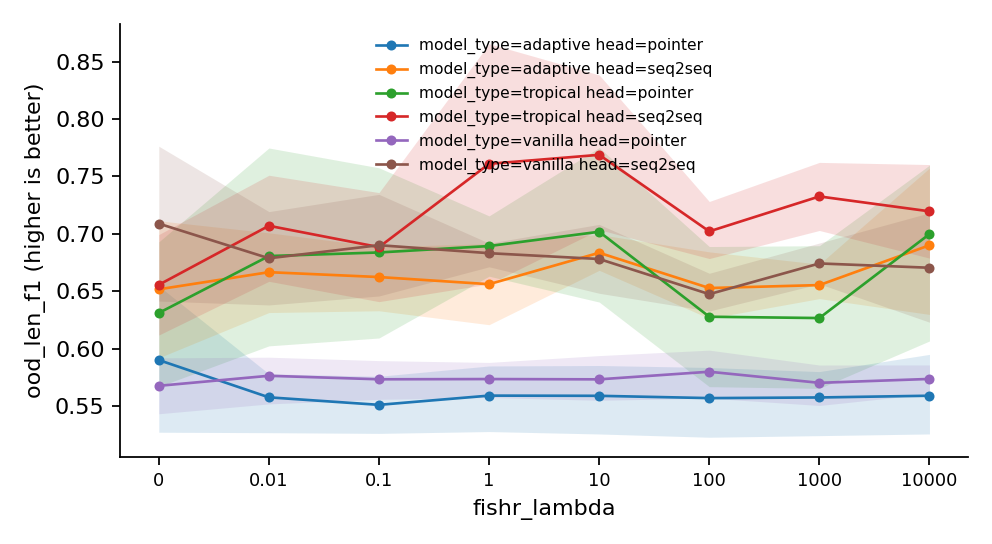
\includegraphics[width=\textwidth]{metric_ood_len_f1.png}
\caption{\texttt{ood\_len\_f1} against \texttt{fishr\_lambda}: the mean over seeds with a 95\% bootstrap CI, one line per combination of the other factors.}
\label{fig:ood_len_f1}
\end{figure}

{\small
\begin{longtable}{lllrlrrr}
\caption{\texttt{ood\_len\_f1} per cell: mean, 95\% bootstrap CI, SD, seeds, diverged runs.}\label{tab:summary-ood_len_f1}\\
\toprule
\texttt{model\_type} & \texttt{head} & \texttt{fishr\_lambda} & mean & 95\% CI & SD & $n$ & div.\\
\midrule
\endhead
adaptive & pointer & 0 & 0.59 & [0.527, 0.655] & 0.0825 & 5 & 0\\
adaptive & pointer & 0.01 & 0.5576 & [0.527, 0.578] & 0.0343 & 5 & 0\\
adaptive & pointer & 0.1 & 0.551 & [0.526, 0.576] & 0.0332 & 5 & 0\\
adaptive & pointer & 1 & 0.5591 & [0.528, 0.585] & 0.0384 & 5 & 0\\
adaptive & pointer & 10 & 0.5589 & [0.526, 0.585] & 0.0386 & 5 & 0\\
adaptive & pointer & 100 & 0.5569 & [0.523, 0.584] & 0.0403 & 5 & 0\\
adaptive & pointer & 1000 & 0.5574 & [0.524, 0.58] & 0.0363 & 5 & 0\\
adaptive & pointer & 1e+04 & 0.559 & [0.526, 0.595] & 0.0476 & 5 & 0\\
adaptive & seq2seq & 0 & 0.6517 & [0.592, 0.711] & 0.0803 & 5 & 0\\
adaptive & seq2seq & 0.01 & 0.6666 & [0.631, 0.701] & 0.0458 & 5 & 0\\
adaptive & seq2seq & 0.1 & 0.6624 & [0.633, 0.689] & 0.036 & 5 & 0\\
adaptive & seq2seq & 1 & 0.6561 & [0.621, 0.691] & 0.0456 & 5 & 0\\
adaptive & seq2seq & 10 & 0.6835 & [0.668, 0.699] & 0.0216 & 5 & 0\\
adaptive & seq2seq & 100 & 0.6528 & [0.626, 0.684] & 0.0377 & 5 & 0\\
adaptive & seq2seq & 1000 & 0.6553 & [0.644, 0.674] & 0.0207 & 5 & 0\\
adaptive & seq2seq & 1e+04 & 0.69 & [0.63, 0.757] & 0.0853 & 5 & 0\\
tropical & pointer & 0 & 0.6311 & [0.567, 0.693] & 0.0832 & 5 & 0\\
tropical & pointer & 0.01 & 0.6806 & [0.602, 0.775] & 0.108 & 5 & 0\\
tropical & pointer & 0.1 & 0.6838 & [0.609, 0.758] & 0.0996 & 5 & 0\\
tropical & pointer & 1 & 0.6894 & [0.663, 0.716] & 0.0363 & 5 & 0\\
tropical & pointer & 10 & 0.7018 & [0.641, 0.775] & 0.0865 & 5 & 0\\
tropical & pointer & 100 & 0.6278 & [0.567, 0.689] & 0.0834 & 5 & 0\\
tropical & pointer & 1000 & 0.6266 & [0.565, 0.69] & 0.0822 & 5 & 0\\
tropical & pointer & 1e+04 & 0.6998 & [0.607, 0.76] & 0.104 & 5 & 0\\
tropical & seq2seq & 0 & 0.6556 & [0.612, 0.699] & 0.0568 & 5 & 0\\
tropical & seq2seq & 0.01 & 0.707 & [0.659, 0.751] & 0.0592 & 5 & 0\\
tropical & seq2seq & 0.1 & 0.6884 & [0.641, 0.736] & 0.0662 & 5 & 0\\
tropical & seq2seq & 1 & 0.761 & [0.656, 0.866] & 0.135 & 5 & 0\\
tropical & seq2seq & 10 & 0.7688 & [0.704, 0.838] & 0.0898 & 5 & 0\\
tropical & seq2seq & 100 & 0.7021 & [0.678, 0.728] & 0.0325 & 5 & 0\\
tropical & seq2seq & 1000 & 0.7326 & [0.703, 0.762] & 0.0385 & 5 & 0\\
tropical & seq2seq & 1e+04 & 0.7196 & [0.679, 0.76] & 0.0525 & 5 & 0\\
vanilla & pointer & 0 & 0.5676 & [0.543, 0.592] & 0.0319 & 5 & 0\\
vanilla & pointer & 0.01 & 0.5763 & [0.552, 0.593] & 0.0272 & 5 & 0\\
vanilla & pointer & 0.1 & 0.5733 & [0.556, 0.59] & 0.0229 & 5 & 0\\
vanilla & pointer & 1 & 0.5735 & [0.557, 0.588] & 0.0207 & 5 & 0\\
vanilla & pointer & 10 & 0.5732 & [0.555, 0.594] & 0.0252 & 5 & 0\\
vanilla & pointer & 100 & 0.5799 & [0.557, 0.599] & 0.0262 & 5 & 0\\
vanilla & pointer & 1000 & 0.5702 & [0.55, 0.586] & 0.0237 & 5 & 0\\
vanilla & pointer & 1e+04 & 0.5736 & [0.561, 0.586] & 0.0163 & 5 & 0\\
vanilla & seq2seq & 0 & 0.7089 & [0.641, 0.776] & 0.0859 & 5 & 0\\
vanilla & seq2seq & 0.01 & 0.6787 & [0.638, 0.719] & 0.0523 & 5 & 0\\
vanilla & seq2seq & 0.1 & 0.6901 & [0.646, 0.734] & 0.0592 & 5 & 0\\
vanilla & seq2seq & 1 & 0.6831 & [0.671, 0.692] & 0.0135 & 5 & 0\\
vanilla & seq2seq & 10 & 0.6781 & [0.648, 0.708] & 0.0404 & 5 & 0\\
vanilla & seq2seq & 100 & 0.6474 & [0.633, 0.666] & 0.0203 & 5 & 0\\
vanilla & seq2seq & 1000 & 0.6742 & [0.656, 0.692] & 0.0226 & 5 & 0\\
vanilla & seq2seq & 1e+04 & 0.6705 & [0.623, 0.718] & 0.0624 & 5 & 0\\
\bottomrule
\end{longtable}
}

{\small
\begin{longtable}{lllrrrl}
\caption{\texttt{ood\_len\_f1}: each level of \texttt{fishr\_lambda} against its control (0), within each combination of the other factors. parametric: Dunnett vs control.}\label{tab:control-ood_len_f1}\\
\toprule
\texttt{model\_type} & \texttt{head} & \texttt{fishr\_lambda} & difference & 95\% CI & $p$ & \\
\midrule
\endhead
adaptive & pointer & 0.01 & -0.03248 & [-0.114, 0.0486] & 0.7910 & \\
adaptive & pointer & 0.1 & -0.03902 & [-0.12, 0.0421] & 0.6383 & \\
adaptive & pointer & 1 & -0.03098 & [-0.112, 0.0501] & 0.8227 & \\
adaptive & pointer & 10 & -0.03115 & [-0.112, 0.0499] & 0.8191 & \\
adaptive & pointer & 100 & -0.03315 & [-0.114, 0.048] & 0.7764 & \\
adaptive & pointer & 1000 & -0.0326 & [-0.114, 0.0485] & 0.7885 & \\
adaptive & pointer & 1e+04 & -0.03108 & [-0.112, 0.05] & 0.8208 & \\
adaptive & seq2seq & 0.01 & 0.01491 & [-0.0757, 0.106] & 0.9974 & \\
adaptive & seq2seq & 0.1 & 0.01067 & [-0.0799, 0.101] & 0.9997 & \\
adaptive & seq2seq & 1 & 0.00445 & [-0.0861, 0.095] & 1.0000 & \\
adaptive & seq2seq & 10 & 0.03182 & [-0.0588, 0.122] & 0.8705 & \\
adaptive & seq2seq & 100 & 0.001083 & [-0.0895, 0.0917] & 1.0000 & \\
adaptive & seq2seq & 1000 & 0.003657 & [-0.0869, 0.0943] & 1.0000 & \\
adaptive & seq2seq & 1e+04 & 0.03836 & [-0.0522, 0.129] & 0.7495 & \\
tropical & pointer & 0.01 & 0.04958 & [-0.104, 0.203] & 0.9078 & \\
tropical & pointer & 0.1 & 0.0527 & [-0.101, 0.206] & 0.8815 & \\
tropical & pointer & 1 & 0.0583 & [-0.0951, 0.212] & 0.8261 & \\
tropical & pointer & 10 & 0.07076 & [-0.0827, 0.224] & 0.6773 & \\
tropical & pointer & 100 & -0.003289 & [-0.157, 0.15] & 1.0000 & \\
tropical & pointer & 1000 & -0.004432 & [-0.158, 0.149] & 1.0000 & \\
tropical & pointer & 1e+04 & 0.06873 & [-0.0847, 0.222] & 0.7031 & \\
tropical & seq2seq & 0.01 & 0.05141 & [-0.0763, 0.179] & 0.7874 & \\
tropical & seq2seq & 0.1 & 0.03281 & [-0.0949, 0.161] & 0.9682 & \\
tropical & seq2seq & 1 & 0.1054 & [-0.0223, 0.233] & 0.1403 & \\
tropical & seq2seq & 10 & 0.1132 & [-0.0145, 0.241] & 0.0993 & \\
tropical & seq2seq & 100 & 0.04652 & [-0.0812, 0.174] & 0.8510 & \\
tropical & seq2seq & 1000 & 0.07698 & [-0.0507, 0.205] & 0.4111 & \\
tropical & seq2seq & 1e+04 & 0.06401 & [-0.0637, 0.192] & 0.5988 & \\
vanilla & pointer & 0.01 & 0.008738 & [-0.0343, 0.0518] & 0.9910 & \\
vanilla & pointer & 0.1 & 0.005685 & [-0.0374, 0.0488] & 0.9993 & \\
vanilla & pointer & 1 & 0.005887 & [-0.0372, 0.049] & 0.9992 & \\
vanilla & pointer & 10 & 0.005638 & [-0.0374, 0.0487] & 0.9994 & \\
vanilla & pointer & 100 & 0.01227 & [-0.0308, 0.0553] & 0.9475 & \\
vanilla & pointer & 1000 & 0.002595 & [-0.0405, 0.0457] & 1.0000 & \\
vanilla & pointer & 1e+04 & 0.00599 & [-0.0371, 0.0491] & 0.9991 & \\
vanilla & seq2seq & 0.01 & -0.0302 & [-0.118, 0.0577] & 0.8812 & \\
vanilla & seq2seq & 0.1 & -0.01878 & [-0.107, 0.0691] & 0.9880 & \\
vanilla & seq2seq & 1 & -0.02575 & [-0.114, 0.0621] & 0.9400 & \\
vanilla & seq2seq & 10 & -0.03082 & [-0.119, 0.057] & 0.8712 & \\
vanilla & seq2seq & 100 & -0.06145 & [-0.149, 0.0264] & 0.2677 & \\
vanilla & seq2seq & 1000 & -0.03469 & [-0.123, 0.0532] & 0.8010 & \\
vanilla & seq2seq & 1e+04 & -0.03844 & [-0.126, 0.0494] & 0.7232 & \\
\bottomrule
\end{longtable}
}

{\small
\begin{longtable}{llrrrrr}
\caption{\texttt{ood\_len\_f1} against log10 \texttt{fishr\_lambda}: parametric: OLS slope t-test, seed-bootstrap CI, with the Jonckheere--Terpstra ordered-trend $\tau$ and $p$.}\label{tab:trend-ood_len_f1}\\
\toprule
\texttt{model\_type} & \texttt{head} & estimate & 95\% CI & $p$ & JT $\tau$ & JT $p$\\
\midrule
\endhead
adaptive & pointer & $5.316\times10^{-4}$ & [-0.00251, 0.00331] & 0.8611 & -0.0171 & 0.9126\\
adaptive & seq2seq & 0.001892 & [-0.00862, 0.0124] & 0.6205 & -0.0248 & 0.8706\\
tropical & pointer & -0.004228 & [-0.0199, 0.0115] & 0.5675 & -0.0648 & 0.6431\\
tropical & seq2seq & 0.002403 & [-0.00689, 0.0123] & 0.7064 & 0.0857 & 0.5161\\
vanilla & pointer & $-2.872\times10^{-4}$ & [-0.00203, 0.00117] & 0.8769 & -0.0514 & 0.7121\\
vanilla & seq2seq & -0.003294 & [-0.00899, 0.00167] & 0.3486 & -0.0705 & 0.6189\\
\bottomrule
\end{longtable}
}

{\small
\begin{longtable}{lrrrl}
\caption{\texttt{ood\_len\_f1}: paired contrasts by seed, Holm-corrected across the cells. parametric: paired t-test by seed, Holm.}\label{tab:paired-ood_len_f1}\\
\toprule
contrast (within) & difference & 95\% CI & $p$ & \\
\midrule
\endhead
\stackcell{model\_type: tropical - vanilla\\\footnotesize head=pointer fishr\_lambda=0 } & 0.06346 & [-0.0621, 0.189] & 1.0000 & \\
\stackcell{model\_type: tropical - vanilla\\\footnotesize head=pointer fishr\_lambda=0.01 } & 0.1043 & [-0.0451, 0.254] & 1.0000 & \\
\stackcell{model\_type: tropical - vanilla\\\footnotesize head=pointer fishr\_lambda=0.1 } & 0.1105 & [-0.0326, 0.254] & 0.9873 & \\
\stackcell{model\_type: tropical - vanilla\\\footnotesize head=pointer fishr\_lambda=1 } & 0.1159 & [0.0545, 0.177] & 0.1014 & \\
\stackcell{model\_type: tropical - vanilla\\\footnotesize head=pointer fishr\_lambda=10 } & 0.1286 & [0.0038, 0.253] & 0.5964 & \\
\stackcell{model\_type: tropical - vanilla\\\footnotesize head=pointer fishr\_lambda=100 } & 0.04791 & [-0.082, 0.178] & 1.0000 & \\
\stackcell{model\_type: tropical - vanilla\\\footnotesize head=pointer fishr\_lambda=1000 } & 0.05644 & [-0.0585, 0.171] & 1.0000 & \\
\stackcell{model\_type: tropical - vanilla\\\footnotesize head=pointer fishr\_lambda=1e+04 } & 0.1262 & [-0.0144, 0.267] & 0.8073 & \\
\stackcell{model\_type: tropical - vanilla\\\footnotesize head=seq2seq fishr\_lambda=0 } & -0.05329 & [-0.197, 0.0904] & 1.0000 & \\
\stackcell{model\_type: tropical - vanilla\\\footnotesize head=seq2seq fishr\_lambda=0.01 } & 0.02831 & [-0.0797, 0.136] & 1.0000 & \\
\stackcell{model\_type: tropical - vanilla\\\footnotesize head=seq2seq fishr\_lambda=0.1 } & -0.0017 & [-0.0968, 0.0934] & 1.0000 & \\
\stackcell{model\_type: tropical - vanilla\\\footnotesize head=seq2seq fishr\_lambda=1 } & 0.07784 & [-0.0814, 0.237] & 1.0000 & \\
\stackcell{model\_type: tropical - vanilla\\\footnotesize head=seq2seq fishr\_lambda=10 } & 0.09075 & [-0.0214, 0.203] & 0.9688 & \\
\stackcell{model\_type: tropical - vanilla\\\footnotesize head=seq2seq fishr\_lambda=100 } & 0.05468 & [0.0072, 0.102] & 0.4948 & \\
\stackcell{model\_type: tropical - vanilla\\\footnotesize head=seq2seq fishr\_lambda=1000 } & 0.05837 & [0.00476, 0.112] & 0.5466 & \\
\stackcell{model\_type: tropical - vanilla\\\footnotesize head=seq2seq fishr\_lambda=1e+04 } & 0.04916 & [-0.0574, 0.156] & 1.0000 & \\
\stackcell{model\_type: adaptive - vanilla\\\footnotesize head=pointer fishr\_lambda=0 } & 0.02244 & [-0.0739, 0.119] & 1.0000 & \\
\stackcell{model\_type: adaptive - vanilla\\\footnotesize head=pointer fishr\_lambda=0.01 } & -0.01877 & [-0.0382, $6.41\times10^{-4}$] & 0.8244 & \\
\stackcell{model\_type: adaptive - vanilla\\\footnotesize head=pointer fishr\_lambda=0.1 } & -0.02226 & [-0.0409, -0.00361] & 0.4727 & \\
\stackcell{model\_type: adaptive - vanilla\\\footnotesize head=pointer fishr\_lambda=1 } & -0.01442 & [-0.0406, 0.0117] & 1.0000 & \\
\stackcell{model\_type: adaptive - vanilla\\\footnotesize head=pointer fishr\_lambda=10 } & -0.01435 & [-0.0369, 0.00818] & 1.0000 & \\
\stackcell{model\_type: adaptive - vanilla\\\footnotesize head=pointer fishr\_lambda=100 } & -0.02297 & [-0.0572, 0.0113] & 1.0000 & \\
\stackcell{model\_type: adaptive - vanilla\\\footnotesize head=pointer fishr\_lambda=1000 } & -0.01275 & [-0.0415, 0.016] & 1.0000 & \\
\stackcell{model\_type: adaptive - vanilla\\\footnotesize head=pointer fishr\_lambda=1e+04 } & -0.01463 & [-0.0619, 0.0327] & 1.0000 & \\
\stackcell{model\_type: adaptive - vanilla\\\footnotesize head=seq2seq fishr\_lambda=0 } & -0.05721 & [-0.145, 0.0309] & 1.0000 & \\
\stackcell{model\_type: adaptive - vanilla\\\footnotesize head=seq2seq fishr\_lambda=0.01 } & -0.0121 & [-0.0868, 0.0626] & 1.0000 & \\
\stackcell{model\_type: adaptive - vanilla\\\footnotesize head=seq2seq fishr\_lambda=0.1 } & -0.02776 & [-0.126, 0.071] & 1.0000 & \\
\stackcell{model\_type: adaptive - vanilla\\\footnotesize head=seq2seq fishr\_lambda=1 } & -0.027 & [-0.0955, 0.0415] & 1.0000 & \\
\stackcell{model\_type: adaptive - vanilla\\\footnotesize head=seq2seq fishr\_lambda=10 } & 0.005433 & [-0.0652, 0.0761] & 1.0000 & \\
\stackcell{model\_type: adaptive - vanilla\\\footnotesize head=seq2seq fishr\_lambda=100 } & 0.005327 & [-0.0557, 0.0663] & 1.0000 & \\
\stackcell{model\_type: adaptive - vanilla\\\footnotesize head=seq2seq fishr\_lambda=1000 } & -0.01886 & [-0.0671, 0.0294] & 1.0000 & \\
\stackcell{model\_type: adaptive - vanilla\\\footnotesize head=seq2seq fishr\_lambda=1e+04 } & 0.01959 & [-0.0899, 0.129] & 1.0000 & \\
\stackcell{head: pointer - seq2seq\\\footnotesize model\_type=adaptive fishr\_lambda=0 } & -0.06164 & [-0.18, 0.0567] & 1.0000 & \\
\stackcell{head: pointer - seq2seq\\\footnotesize model\_type=adaptive fishr\_lambda=0.01 } & -0.109 & [-0.186, -0.0324] & 0.2621 & \\
\stackcell{head: pointer - seq2seq\\\footnotesize model\_type=adaptive fishr\_lambda=0.1 } & -0.1113 & [-0.172, -0.0508] & 0.1318 & \\
\stackcell{head: pointer - seq2seq\\\footnotesize model\_type=adaptive fishr\_lambda=1 } & -0.09707 & [-0.178, -0.0161] & 0.3495 & \\
\stackcell{head: pointer - seq2seq\\\footnotesize model\_type=adaptive fishr\_lambda=10 } & -0.1246 & [-0.18, -0.0693] & 0.0765 & \\
\stackcell{head: pointer - seq2seq\\\footnotesize model\_type=adaptive fishr\_lambda=100 } & -0.09587 & [-0.144, -0.0475] & 0.1115 & \\
\stackcell{head: pointer - seq2seq\\\footnotesize model\_type=adaptive fishr\_lambda=1000 } & -0.0979 & [-0.145, -0.0507] & 0.0992 & \\
\stackcell{head: pointer - seq2seq\\\footnotesize model\_type=adaptive fishr\_lambda=1e+04 } & -0.1311 & [-0.207, -0.0553] & 0.1553 & \\
\stackcell{head: pointer - seq2seq\\\footnotesize model\_type=tropical fishr\_lambda=0 } & -0.02454 & [-0.162, 0.113] & 1.0000 & \\
\stackcell{head: pointer - seq2seq\\\footnotesize model\_type=tropical fishr\_lambda=0.01 } & -0.02637 & [-0.0993, 0.0465] & 1.0000 & \\
\stackcell{head: pointer - seq2seq\\\footnotesize model\_type=tropical fishr\_lambda=0.1 } & -0.004646 & [-0.109, 0.0994] & 1.0000 & \\
\stackcell{head: pointer - seq2seq\\\footnotesize model\_type=tropical fishr\_lambda=1 } & -0.07162 & [-0.235, 0.0913] & 1.0000 & \\
\stackcell{head: pointer - seq2seq\\\footnotesize model\_type=tropical fishr\_lambda=10 } & -0.06699 & [-0.281, 0.147] & 1.0000 & \\
\stackcell{head: pointer - seq2seq\\\footnotesize model\_type=tropical fishr\_lambda=100 } & -0.07435 & [-0.173, 0.0241] & 0.8332 & \\
\stackcell{head: pointer - seq2seq\\\footnotesize model\_type=tropical fishr\_lambda=1000 } & -0.1059 & [-0.216, 0.00415] & 0.5013 & \\
\stackcell{head: pointer - seq2seq\\\footnotesize model\_type=tropical fishr\_lambda=1e+04 } & -0.01981 & [-0.142, 0.102] & 1.0000 & \\
\stackcell{head: pointer - seq2seq\\\footnotesize model\_type=vanilla fishr\_lambda=0 } & -0.1413 & [-0.252, -0.0301] & 0.3394 & \\
\stackcell{head: pointer - seq2seq\\\footnotesize model\_type=vanilla fishr\_lambda=0.01 } & -0.1024 & [-0.193, -0.0121] & 0.3807 & \\
\stackcell{head: pointer - seq2seq\\\footnotesize model\_type=vanilla fishr\_lambda=0.1 } & -0.1168 & [-0.194, -0.0401] & 0.2281 & \\
\stackcell{head: pointer - seq2seq\\\footnotesize model\_type=vanilla fishr\_lambda=1 } & -0.1096 & [-0.146, -0.0729] & 0.0278 & *\\
\stackcell{head: pointer - seq2seq\\\footnotesize model\_type=vanilla fishr\_lambda=10 } & -0.1048 & [-0.178, -0.0317] & 0.2621 & \\
\stackcell{head: pointer - seq2seq\\\footnotesize model\_type=vanilla fishr\_lambda=100 } & -0.06758 & [-0.121, -0.0137] & 0.3394 & \\
\stackcell{head: pointer - seq2seq\\\footnotesize model\_type=vanilla fishr\_lambda=1000 } & -0.104 & [-0.158, -0.0503] & 0.1154 & \\
\stackcell{head: pointer - seq2seq\\\footnotesize model\_type=vanilla fishr\_lambda=1e+04 } & -0.09686 & [-0.183, -0.0103] & 0.3807 & \\
\bottomrule
\end{longtable}
}

\clearpage
\appendix
\section{Other metrics}
\subsection{\texttt{ood\_len\_exact}}
\begin{figure}[tbp]
\centering
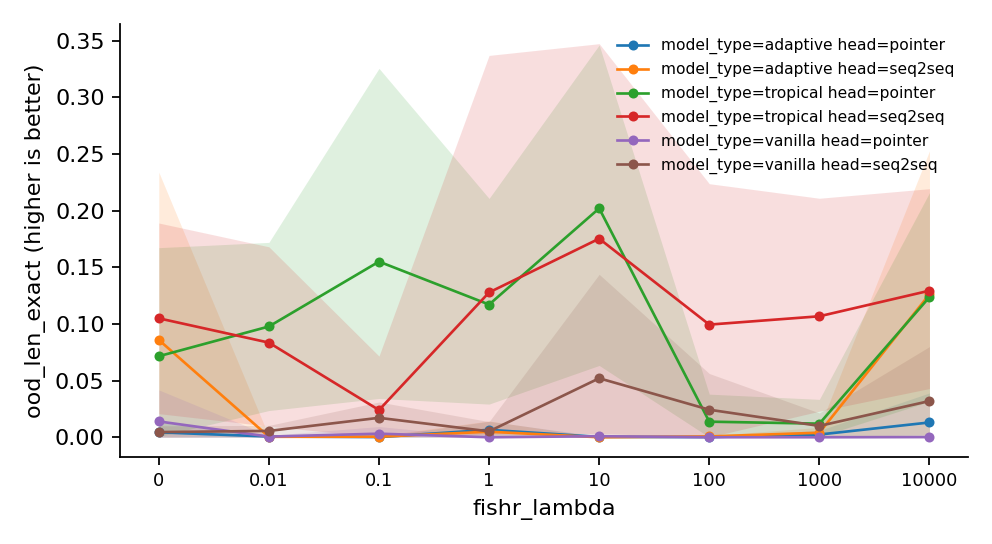
\includegraphics[width=\textwidth]{metric_ood_len_exact.png}
\caption{\texttt{ood\_len\_exact} against \texttt{fishr\_lambda}: the mean over seeds with a 95\% bootstrap CI, one line per combination of the other factors.}
\label{fig:ood_len_exact}
\end{figure}

{\small
\begin{longtable}{lllrlrrr}
\caption{\texttt{ood\_len\_exact} per cell: mean, 95\% bootstrap CI, SD, seeds, diverged runs.}\label{tab:summary-ood_len_exact}\\
\toprule
\texttt{model\_type} & \texttt{head} & \texttt{fishr\_lambda} & mean & 95\% CI & SD & $n$ & div.\\
\midrule
\endhead
adaptive & pointer & 0 & 0.00435 & [0, 0.0131] & 0.00973 & 5 & 0\\
adaptive & pointer & 0.01 & $6.500\times10^{-4}$ & [0, 0.00145] & $9.29\times10^{-4}$ & 5 & 0\\
adaptive & pointer & 0.1 & $1.500\times10^{-4}$ & [0, $3.50\times10^{-4}$] & $2.24\times10^{-4}$ & 5 & 0\\
adaptive & pointer & 1 & 0.00655 & [0, 0.014] & 0.00912 & 5 & 0\\
adaptive & pointer & 10 & $3.000\times10^{-4}$ & [0, $9.00\times10^{-4}$] & $6.71\times10^{-4}$ & 5 & 0\\
adaptive & pointer & 100 & $1.500\times10^{-4}$ & [0, $4.50\times10^{-4}$] & $3.35\times10^{-4}$ & 5 & 0\\
adaptive & pointer & 1000 & 0.0024 & [0, 0.006] & 0.00391 & 5 & 0\\
adaptive & pointer & 1e+04 & 0.01305 & [0, 0.0392] & 0.0292 & 5 & 0\\
adaptive & seq2seq & 0 & 0.0859 & [$2.00\times10^{-4}$, 0.234] & 0.161 & 5 & 0\\
adaptive & seq2seq & 0.01 & $4.000\times10^{-4}$ & [0, $8.00\times10^{-4}$] & $5.48\times10^{-4}$ & 5 & 0\\
adaptive & seq2seq & 0.1 & $5.000\times10^{-4}$ & [0, 0.0014] & $9.84\times10^{-4}$ & 5 & 0\\
adaptive & seq2seq & 1 & 0.0049 & [0, 0.0144] & 0.0107 & 5 & 0\\
adaptive & seq2seq & 10 & 0 & [0, 0] & 0 & 5 & 0\\
adaptive & seq2seq & 100 & $7.000\times10^{-4}$ & [0, 0.0014] & $9.59\times10^{-4}$ & 5 & 0\\
adaptive & seq2seq & 1000 & 0.004 & [$5.00\times10^{-5}$, 0.00875] & 0.00557 & 5 & 0\\
adaptive & seq2seq & 1e+04 & 0.1261 & [$5.00\times10^{-4}$, 0.253] & 0.172 & 5 & 0\\
tropical & pointer & 0 & 0.0715 & [$6.50\times10^{-4}$, 0.167] & 0.12 & 5 & 0\\
tropical & pointer & 0.01 & 0.09775 & [0.0236, 0.172] & 0.0949 & 5 & 0\\
tropical & pointer & 0.1 & 0.155 & [0.0342, 0.326] & 0.196 & 5 & 0\\
tropical & pointer & 1 & 0.1171 & [0.0292, 0.211] & 0.116 & 5 & 0\\
tropical & pointer & 10 & 0.202 & [0.0634, 0.346] & 0.185 & 5 & 0\\
tropical & pointer & 100 & 0.01375 & [0, 0.0381] & 0.0265 & 5 & 0\\
tropical & pointer & 1000 & 0.012 & [$4.50\times10^{-4}$, 0.0335] & 0.0239 & 5 & 0\\
tropical & pointer & 1e+04 & 0.1237 & [0.0316, 0.216] & 0.12 & 5 & 0\\
tropical & seq2seq & 0 & 0.105 & [0.0209, 0.189] & 0.106 & 5 & 0\\
tropical & seq2seq & 0.01 & 0.0835 & [0.00975, 0.168] & 0.101 & 5 & 0\\
tropical & seq2seq & 0.1 & 0.024 & [0, 0.0716] & 0.0531 & 5 & 0\\
tropical & seq2seq & 1 & 0.1278 & [0.0028, 0.337] & 0.228 & 5 & 0\\
tropical & seq2seq & 10 & 0.1752 & [0.00325, 0.347] & 0.233 & 5 & 0\\
tropical & seq2seq & 100 & 0.0994 & [$1.50\times10^{-4}$, 0.224] & 0.143 & 5 & 0\\
tropical & seq2seq & 1000 & 0.1067 & [0.023, 0.211] & 0.118 & 5 & 0\\
tropical & seq2seq & 1e+04 & 0.1294 & [0.043, 0.219] & 0.117 & 5 & 0\\
vanilla & pointer & 0 & 0.01395 & [0, 0.0418] & 0.0311 & 5 & 0\\
vanilla & pointer & 0.01 & $5.500\times10^{-4}$ & [0, 0.00165] & 0.00123 & 5 & 0\\
vanilla & pointer & 0.1 & 0.00315 & [0, 0.00945] & 0.00704 & 5 & 0\\
vanilla & pointer & 1 & 0 & [0, 0] & 0 & 5 & 0\\
vanilla & pointer & 10 & $9.000\times10^{-4}$ & [0, 0.0027] & 0.00201 & 5 & 0\\
vanilla & pointer & 100 & 0 & [0, 0] & 0 & 5 & 0\\
vanilla & pointer & 1000 & 0 & [0, 0] & 0 & 5 & 0\\
vanilla & pointer & 1e+04 & $1.500\times10^{-4}$ & [0, $4.50\times10^{-4}$] & $3.35\times10^{-4}$ & 5 & 0\\
vanilla & seq2seq & 0 & 0.00455 & [$5.00\times10^{-5}$, 0.0101] & 0.00642 & 5 & 0\\
vanilla & seq2seq & 0.01 & 0.0056 & [$7.50\times10^{-4}$, 0.0105] & 0.00629 & 5 & 0\\
vanilla & seq2seq & 0.1 & 0.01715 & [0.0034, 0.0311] & 0.0182 & 5 & 0\\
vanilla & seq2seq & 1 & 0.0052 & [$1.00\times10^{-4}$, 0.0138] & 0.00938 & 5 & 0\\
vanilla & seq2seq & 10 & 0.05205 & [0.0019, 0.144] & 0.102 & 5 & 0\\
vanilla & seq2seq & 100 & 0.0243 & [0, 0.0563] & 0.0406 & 5 & 0\\
vanilla & seq2seq & 1000 & 0.01 & [$4.50\times10^{-4}$, 0.0215] & 0.0134 & 5 & 0\\
vanilla & seq2seq & 1e+04 & 0.03195 & [0.00215, 0.08] & 0.0521 & 5 & 0\\
\bottomrule
\end{longtable}
}

{\small
\begin{longtable}{lllrrrl}
\caption{\texttt{ood\_len\_exact}: each level of \texttt{fishr\_lambda} against its control (0), within each combination of the other factors. rank: Wilcoxon signed-rank by seed, Holm.}\label{tab:control-ood_len_exact}\\
\toprule
\texttt{model\_type} & \texttt{head} & \texttt{fishr\_lambda} & difference & 95\% CI & $p$ & \\
\midrule
\endhead
adaptive & pointer & 0.01 & 0 & [-0.0128, 0.0014] & 1.0000 & \\
adaptive & pointer & 0.1 & 0 & [-0.013, $3.01\times10^{-4}$] & 1.0000 & \\
adaptive & pointer & 1 & 0 & [-0.0102, 0.014] & 1.0000 & \\
adaptive & pointer & 10 & 0 & [-0.0131, $9.00\times10^{-4}$] & 1.0000 & \\
adaptive & pointer & 100 & 0 & [-0.0131, $4.50\times10^{-4}$] & 1.0000 & \\
adaptive & pointer & 1000 & 0 & [-0.0124, 0.0054] & 1.0000 & \\
adaptive & pointer & 1e+04 & 0 & [-0.0131, 0.0392] & 1.0000 & \\
adaptive & seq2seq & 0.01 & -0.001 & [-0.233, $2.00\times10^{-4}$] & 1.0000 & \\
adaptive & seq2seq & 0.1 & -0.001 & [-0.233, $-1.49\times10^{-4}$] & 1.0000 & \\
adaptive & seq2seq & 1 & -0.001 & [-0.229, 0.0096] & 1.0000 & \\
adaptive & seq2seq & 10 & -0.001 & [-0.234, $-2.00\times10^{-4}$] & 1.0000 & \\
adaptive & seq2seq & 100 & -0.001 & [-0.233, $-2.00\times10^{-4}$] & 1.0000 & \\
adaptive & seq2seq & 1000 & $-7.500\times10^{-4}$ & [-0.225, $-1.50\times10^{-4}$] & 1.0000 & \\
adaptive & seq2seq & 1e+04 & $5.000\times10^{-4}$ & [-0.222, 0.229] & 1.0000 & \\
tropical & pointer & 0.01 & 0.004 & [-0.0313, 0.0956] & 1.0000 & \\
tropical & pointer & 0.1 & 0.0825 & [0.0255, 0.148] & 0.8750 & \\
tropical & pointer & 1 & $7.500\times10^{-4}$ & [-0.00445, 0.102] & 1.0000 & \\
tropical & pointer & 10 & 0.0505 & [0.0157, 0.281] & 0.8750 & \\
tropical & pointer & 100 & -0.00325 & [-0.144, 0.0032] & 1.0000 & \\
tropical & pointer & 1000 & -0.00325 & [-0.169, $6.00\times10^{-4}$] & 1.0000 & \\
tropical & pointer & 1e+04 & 0.03525 & [-0.0185, 0.133] & 1.0000 & \\
tropical & seq2seq & 0.01 & 0 & [-0.105, 0.0586] & 1.0000 & \\
tropical & seq2seq & 0.1 & -0.1003 & [-0.189, 0.0328] & 1.0000 & \\
tropical & seq2seq & 1 & -0.099 & [-0.184, 0.3] & 1.0000 & \\
tropical & seq2seq & 10 & -0.0015 & [-0.127, 0.288] & 1.0000 & \\
tropical & seq2seq & 100 & -0.045 & [-0.133, 0.165] & 1.0000 & \\
tropical & seq2seq & 1000 & 0.011 & [-0.086, 0.0983] & 1.0000 & \\
tropical & seq2seq & 1e+04 & 0.03725 & [-0.012, 0.062] & 1.0000 & \\
vanilla & pointer & 0.01 & 0 & [-0.0417, 0.0016] & 1.0000 & \\
vanilla & pointer & 0.1 & 0 & [-0.0323, 0] & 1.0000 & \\
vanilla & pointer & 1 & 0 & [-0.0418, 0] & 1.0000 & \\
vanilla & pointer & 10 & 0 & [-0.0391, 0] & 1.0000 & \\
vanilla & pointer & 100 & 0 & [-0.0418, 0] & 1.0000 & \\
vanilla & pointer & 1000 & 0 & [-0.0418, 0] & 1.0000 & \\
vanilla & pointer & 1e+04 & 0 & [-0.0413, 0] & 1.0000 & \\
vanilla & seq2seq & 0.01 & 0 & [-0.0031, 0.00625] & 1.0000 & \\
vanilla & seq2seq & 0.1 & 0.004 & [$8.00\times10^{-4}$, 0.0244] & 1.0000 & \\
vanilla & seq2seq & 1 & 0 & [-0.0075, 0.0131] & 1.0000 & \\
vanilla & seq2seq & 10 & 0.00825 & [0.00165, 0.134] & 1.0000 & \\
vanilla & seq2seq & 100 & 0 & [-0.0034, 0.0571] & 1.0000 & \\
vanilla & seq2seq & 1000 & 0.00225 & [$3.50\times10^{-4}$, 0.0135] & 1.0000 & \\
vanilla & seq2seq & 1e+04 & 0.0045 & [-0.0017, 0.0669] & 1.0000 & \\
\bottomrule
\end{longtable}
}

{\small
\begin{longtable}{llrrrrr}
\caption{\texttt{ood\_len\_exact} against log10 \texttt{fishr\_lambda}: rank: Spearman rho, seed-bootstrap CI, with the Jonckheere--Terpstra ordered-trend $\tau$ and $p$.}\label{tab:trend-ood_len_exact}\\
\toprule
\texttt{model\_type} & \texttt{head} & estimate & 95\% CI & $p$ & JT $\tau$ & JT $p$\\
\midrule
\endhead
adaptive & pointer & -0.06013 & [-0.291, 0.171] & 0.7315 & -0.04 & 0.7249\\
adaptive & seq2seq & 0.3337 & [-0.0681, 0.729] & 0.0501 & 0.238 & 0.0516\\
tropical & pointer & -0.1942 & [-0.393, 0.0302] & 0.2635 & -0.133 & 0.3173\\
tropical & seq2seq & 0.2526 & [-0.0076, 0.526] & 0.1432 & 0.185 & 0.1654\\
vanilla & pointer & -0.105 & [-0.459, 0.0364] & 0.5485 & -0.0419 & 0.5745\\
vanilla & seq2seq & 0.03393 & [-0.234, 0.283] & 0.8466 & 0.0286 & 0.8216\\
\bottomrule
\end{longtable}
}

{\small
\begin{longtable}{lrrrl}
\caption{\texttt{ood\_len\_exact}: paired contrasts by seed, Holm-corrected across the cells. rank: Wilcoxon signed-rank by seed, Holm.}\label{tab:paired-ood_len_exact}\\
\toprule
contrast (within) & difference & 95\% CI & $p$ & \\
\midrule
\endhead
\stackcell{model\_type: tropical - vanilla\\\footnotesize head=pointer fishr\_lambda=0 } & 0.05755 & [-0.108, 0.223] & 1.0000 & \\
\stackcell{model\_type: tropical - vanilla\\\footnotesize head=pointer fishr\_lambda=0.01 } & 0.0972 & [-0.0214, 0.216] & 1.0000 & \\
\stackcell{model\_type: tropical - vanilla\\\footnotesize head=pointer fishr\_lambda=0.1 } & 0.1518 & [-0.0931, 0.397] & 1.0000 & \\
\stackcell{model\_type: tropical - vanilla\\\footnotesize head=pointer fishr\_lambda=1 } & 0.1171 & [-0.0265, 0.261] & 1.0000 & \\
\stackcell{model\_type: tropical - vanilla\\\footnotesize head=pointer fishr\_lambda=10 } & 0.2011 & [-0.03, 0.432] & 1.0000 & \\
\stackcell{model\_type: tropical - vanilla\\\footnotesize head=pointer fishr\_lambda=100 } & 0.01375 & [-0.0192, 0.0467] & 1.0000 & \\
\stackcell{model\_type: tropical - vanilla\\\footnotesize head=pointer fishr\_lambda=1000 } & 0.012 & [-0.0177, 0.0417] & 1.0000 & \\
\stackcell{model\_type: tropical - vanilla\\\footnotesize head=pointer fishr\_lambda=1e+04 } & 0.1236 & [-0.0255, 0.273] & 1.0000 & \\
\stackcell{model\_type: tropical - vanilla\\\footnotesize head=seq2seq fishr\_lambda=0 } & 0.1004 & [-0.0294, 0.23] & 1.0000 & \\
\stackcell{model\_type: tropical - vanilla\\\footnotesize head=seq2seq fishr\_lambda=0.01 } & 0.0779 & [-0.0466, 0.202] & 1.0000 & \\
\stackcell{model\_type: tropical - vanilla\\\footnotesize head=seq2seq fishr\_lambda=0.1 } & 0.00685 & [-0.0525, 0.0662] & 1.0000 & \\
\stackcell{model\_type: tropical - vanilla\\\footnotesize head=seq2seq fishr\_lambda=1 } & 0.1226 & [-0.149, 0.395] & 1.0000 & \\
\stackcell{model\_type: tropical - vanilla\\\footnotesize head=seq2seq fishr\_lambda=10 } & 0.1232 & [-0.236, 0.483] & 1.0000 & \\
\stackcell{model\_type: tropical - vanilla\\\footnotesize head=seq2seq fishr\_lambda=100 } & 0.0751 & [-0.0979, 0.248] & 1.0000 & \\
\stackcell{model\_type: tropical - vanilla\\\footnotesize head=seq2seq fishr\_lambda=1000 } & 0.09675 & [-0.0597, 0.253] & 1.0000 & \\
\stackcell{model\_type: tropical - vanilla\\\footnotesize head=seq2seq fishr\_lambda=1e+04 } & 0.0974 & [-0.09, 0.285] & 1.0000 & \\
\stackcell{model\_type: adaptive - vanilla\\\footnotesize head=pointer fishr\_lambda=0 } & -0.0096 & [-0.0528, 0.0336] & 1.0000 & \\
\stackcell{model\_type: adaptive - vanilla\\\footnotesize head=pointer fishr\_lambda=0.01 } & $1.000\times10^{-4}$ & [-0.00214, 0.00234] & 1.0000 & \\
\stackcell{model\_type: adaptive - vanilla\\\footnotesize head=pointer fishr\_lambda=0.1 } & -0.003 & [-0.0115, 0.0055] & 1.0000 & \\
\stackcell{model\_type: adaptive - vanilla\\\footnotesize head=pointer fishr\_lambda=1 } & 0.00655 & [-0.00478, 0.0179] & 1.0000 & \\
\stackcell{model\_type: adaptive - vanilla\\\footnotesize head=pointer fishr\_lambda=10 } & $-6.000\times10^{-4}$ & [-0.00227, 0.00107] & 1.0000 & \\
\stackcell{model\_type: adaptive - vanilla\\\footnotesize head=pointer fishr\_lambda=100 } & $1.500\times10^{-4}$ & [$-2.66\times10^{-4}$, $5.66\times10^{-4}$] & 1.0000 & \\
\stackcell{model\_type: adaptive - vanilla\\\footnotesize head=pointer fishr\_lambda=1000 } & 0.0024 & [-0.00246, 0.00726] & 1.0000 & \\
\stackcell{model\_type: adaptive - vanilla\\\footnotesize head=pointer fishr\_lambda=1e+04 } & 0.0129 & [-0.0229, 0.0487] & 1.0000 & \\
\stackcell{model\_type: adaptive - vanilla\\\footnotesize head=seq2seq fishr\_lambda=0 } & 0.08135 & [-0.122, 0.284] & 1.0000 & \\
\stackcell{model\_type: adaptive - vanilla\\\footnotesize head=seq2seq fishr\_lambda=0.01 } & -0.0052 & [-0.0131, 0.00265] & 1.0000 & \\
\stackcell{model\_type: adaptive - vanilla\\\footnotesize head=seq2seq fishr\_lambda=0.1 } & -0.01665 & [-0.0388, 0.00551] & 1.0000 & \\
\stackcell{model\_type: adaptive - vanilla\\\footnotesize head=seq2seq fishr\_lambda=1 } & $-3.000\times10^{-4}$ & [-0.0203, 0.0197] & 1.0000 & \\
\stackcell{model\_type: adaptive - vanilla\\\footnotesize head=seq2seq fishr\_lambda=10 } & -0.05205 & [-0.179, 0.0745] & 1.0000 & \\
\stackcell{model\_type: adaptive - vanilla\\\footnotesize head=seq2seq fishr\_lambda=100 } & -0.0236 & [-0.0747, 0.0275] & 1.0000 & \\
\stackcell{model\_type: adaptive - vanilla\\\footnotesize head=seq2seq fishr\_lambda=1000 } & -0.006 & [-0.0227, 0.0107] & 1.0000 & \\
\stackcell{model\_type: adaptive - vanilla\\\footnotesize head=seq2seq fishr\_lambda=1e+04 } & 0.0942 & [-0.094, 0.282] & 1.0000 & \\
\stackcell{head: pointer - seq2seq\\\footnotesize model\_type=adaptive fishr\_lambda=0 } & -0.08155 & [-0.285, 0.122] & 1.0000 & \\
\stackcell{head: pointer - seq2seq\\\footnotesize model\_type=adaptive fishr\_lambda=0.01 } & $2.500\times10^{-4}$ & [-0.00142, 0.00192] & 1.0000 & \\
\stackcell{head: pointer - seq2seq\\\footnotesize model\_type=adaptive fishr\_lambda=0.1 } & $-3.500\times10^{-4}$ & [-0.00171, 0.00101] & 1.0000 & \\
\stackcell{head: pointer - seq2seq\\\footnotesize model\_type=adaptive fishr\_lambda=1 } & 0.00165 & [-0.019, 0.0223] & 1.0000 & \\
\stackcell{head: pointer - seq2seq\\\footnotesize model\_type=adaptive fishr\_lambda=10 } & $3.000\times10^{-4}$ & [$-5.33\times10^{-4}$, 0.00113] & 1.0000 & \\
\stackcell{head: pointer - seq2seq\\\footnotesize model\_type=adaptive fishr\_lambda=100 } & $-5.500\times10^{-4}$ & [-0.00154, $4.41\times10^{-4}$] & 1.0000 & \\
\stackcell{head: pointer - seq2seq\\\footnotesize model\_type=adaptive fishr\_lambda=1000 } & -0.0016 & [-0.00895, 0.00575] & 1.0000 & \\
\stackcell{head: pointer - seq2seq\\\footnotesize model\_type=adaptive fishr\_lambda=1e+04 } & -0.1131 & [-0.307, 0.0808] & 1.0000 & \\
\stackcell{head: pointer - seq2seq\\\footnotesize model\_type=tropical fishr\_lambda=0 } & -0.03345 & [-0.146, 0.079] & 1.0000 & \\
\stackcell{head: pointer - seq2seq\\\footnotesize model\_type=tropical fishr\_lambda=0.01 } & 0.01425 & [-0.112, 0.14] & 1.0000 & \\
\stackcell{head: pointer - seq2seq\\\footnotesize model\_type=tropical fishr\_lambda=0.1 } & 0.131 & [-0.142, 0.404] & 1.0000 & \\
\stackcell{head: pointer - seq2seq\\\footnotesize model\_type=tropical fishr\_lambda=1 } & -0.0107 & [-0.407, 0.385] & 1.0000 & \\
\stackcell{head: pointer - seq2seq\\\footnotesize model\_type=tropical fishr\_lambda=10 } & 0.02675 & [-0.487, 0.54] & 1.0000 & \\
\stackcell{head: pointer - seq2seq\\\footnotesize model\_type=tropical fishr\_lambda=100 } & -0.08565 & [-0.256, 0.0851] & 1.0000 & \\
\stackcell{head: pointer - seq2seq\\\footnotesize model\_type=tropical fishr\_lambda=1000 } & -0.09475 & [-0.252, 0.0621] & 1.0000 & \\
\stackcell{head: pointer - seq2seq\\\footnotesize model\_type=tropical fishr\_lambda=1e+04 } & -0.00565 & [-0.18, 0.168] & 1.0000 & \\
\stackcell{head: pointer - seq2seq\\\footnotesize model\_type=vanilla fishr\_lambda=0 } & 0.0094 & [-0.0272, 0.046] & 1.0000 & \\
\stackcell{head: pointer - seq2seq\\\footnotesize model\_type=vanilla fishr\_lambda=0.01 } & -0.00505 & [-0.0137, 0.0036] & 1.0000 & \\
\stackcell{head: pointer - seq2seq\\\footnotesize model\_type=vanilla fishr\_lambda=0.1 } & -0.014 & [-0.0403, 0.0123] & 1.0000 & \\
\stackcell{head: pointer - seq2seq\\\footnotesize model\_type=vanilla fishr\_lambda=1 } & -0.0052 & [-0.0169, 0.00645] & 1.0000 & \\
\stackcell{head: pointer - seq2seq\\\footnotesize model\_type=vanilla fishr\_lambda=10 } & -0.05115 & [-0.178, 0.076] & 1.0000 & \\
\stackcell{head: pointer - seq2seq\\\footnotesize model\_type=vanilla fishr\_lambda=100 } & -0.0243 & [-0.0748, 0.0262] & 1.0000 & \\
\stackcell{head: pointer - seq2seq\\\footnotesize model\_type=vanilla fishr\_lambda=1000 } & -0.01 & [-0.0266, 0.00659] & 1.0000 & \\
\stackcell{head: pointer - seq2seq\\\footnotesize model\_type=vanilla fishr\_lambda=1e+04 } & -0.0318 & [-0.0966, 0.033] & 1.0000 & \\
\bottomrule
\end{longtable}
}

\subsection{\texttt{ood\_val\_f1}}
\begin{figure}[tbp]
\centering
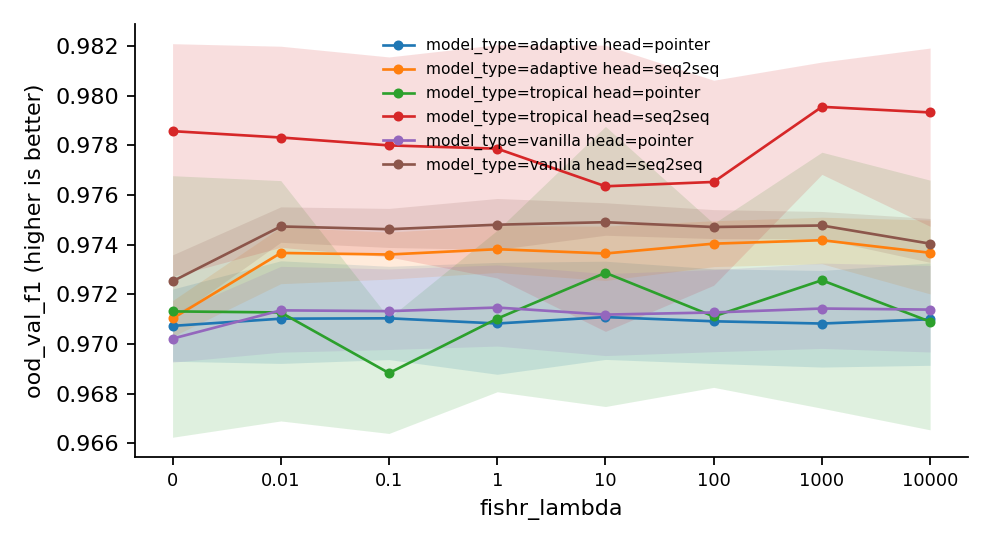
\includegraphics[width=\textwidth]{metric_ood_val_f1.png}
\caption{\texttt{ood\_val\_f1} against \texttt{fishr\_lambda}: the mean over seeds with a 95\% bootstrap CI, one line per combination of the other factors.}
\label{fig:ood_val_f1}
\end{figure}

{\small
\begin{longtable}{lllrlrrr}
\caption{\texttt{ood\_val\_f1} per cell: mean, 95\% bootstrap CI, SD, seeds, diverged runs.}\label{tab:summary-ood_val_f1}\\
\toprule
\texttt{model\_type} & \texttt{head} & \texttt{fishr\_lambda} & mean & 95\% CI & SD & $n$ & div.\\
\midrule
\endhead
adaptive & pointer & 0 & 0.9707 & [0.969, 0.972] & 0.00194 & 5 & 0\\
adaptive & pointer & 0.01 & 0.971 & [0.969, 0.973] & 0.00261 & 5 & 0\\
adaptive & pointer & 0.1 & 0.971 & [0.969, 0.973] & 0.00243 & 5 & 0\\
adaptive & pointer & 1 & 0.9708 & [0.969, 0.973] & 0.00289 & 5 & 0\\
adaptive & pointer & 10 & 0.9711 & [0.969, 0.973] & 0.00251 & 5 & 0\\
adaptive & pointer & 100 & 0.9709 & [0.969, 0.973] & 0.00243 & 5 & 0\\
adaptive & pointer & 1000 & 0.9708 & [0.969, 0.973] & 0.00247 & 5 & 0\\
adaptive & pointer & 1e+04 & 0.971 & [0.969, 0.973] & 0.00258 & 5 & 0\\
adaptive & seq2seq & 0 & 0.971 & [0.97, 0.972] & $8.96\times10^{-4}$ & 5 & 0\\
adaptive & seq2seq & 0.01 & 0.9737 & [0.972, 0.975] & 0.00144 & 5 & 0\\
adaptive & seq2seq & 0.1 & 0.9736 & [0.973, 0.975] & 0.00121 & 5 & 0\\
adaptive & seq2seq & 1 & 0.9738 & [0.973, 0.975] & 0.00132 & 5 & 0\\
adaptive & seq2seq & 10 & 0.9736 & [0.973, 0.975] & 0.00145 & 5 & 0\\
adaptive & seq2seq & 100 & 0.974 & [0.973, 0.975] & 0.00117 & 5 & 0\\
adaptive & seq2seq & 1000 & 0.9742 & [0.973, 0.975] & 0.00123 & 5 & 0\\
adaptive & seq2seq & 1e+04 & 0.9737 & [0.972, 0.975] & 0.00184 & 5 & 0\\
tropical & pointer & 0 & 0.9713 & [0.966, 0.977] & 0.00697 & 5 & 0\\
tropical & pointer & 0.01 & 0.9713 & [0.967, 0.977] & 0.00636 & 5 & 0\\
tropical & pointer & 0.1 & 0.9688 & [0.966, 0.971] & 0.00299 & 5 & 0\\
tropical & pointer & 1 & 0.971 & [0.968, 0.975] & 0.00412 & 5 & 0\\
tropical & pointer & 10 & 0.9729 & [0.967, 0.979] & 0.00717 & 5 & 0\\
tropical & pointer & 100 & 0.9711 & [0.968, 0.975] & 0.0043 & 5 & 0\\
tropical & pointer & 1000 & 0.9726 & [0.967, 0.978] & 0.0067 & 5 & 0\\
tropical & pointer & 1e+04 & 0.9709 & [0.967, 0.977] & 0.00676 & 5 & 0\\
tropical & seq2seq & 0 & 0.9786 & [0.973, 0.982] & 0.00649 & 5 & 0\\
tropical & seq2seq & 0.01 & 0.9783 & [0.974, 0.982] & 0.00513 & 5 & 0\\
tropical & seq2seq & 0.1 & 0.978 & [0.974, 0.982] & 0.00519 & 5 & 0\\
tropical & seq2seq & 1 & 0.9779 & [0.973, 0.982] & 0.00649 & 5 & 0\\
tropical & seq2seq & 10 & 0.9763 & [0.971, 0.982] & 0.0076 & 5 & 0\\
tropical & seq2seq & 100 & 0.9765 & [0.972, 0.981] & 0.00531 & 5 & 0\\
tropical & seq2seq & 1000 & 0.9795 & [0.977, 0.981] & 0.00282 & 5 & 0\\
tropical & seq2seq & 1e+04 & 0.9793 & [0.975, 0.982] & 0.005 & 5 & 0\\
vanilla & pointer & 0 & 0.9702 & [0.969, 0.971] & 0.0013 & 5 & 0\\
vanilla & pointer & 0.01 & 0.9714 & [0.97, 0.973] & 0.00236 & 5 & 0\\
vanilla & pointer & 0.1 & 0.9713 & [0.97, 0.973] & 0.00222 & 5 & 0\\
vanilla & pointer & 1 & 0.9715 & [0.97, 0.973] & 0.00203 & 5 & 0\\
vanilla & pointer & 10 & 0.9712 & [0.97, 0.973] & 0.00224 & 5 & 0\\
vanilla & pointer & 100 & 0.9713 & [0.97, 0.973] & 0.00213 & 5 & 0\\
vanilla & pointer & 1000 & 0.9714 & [0.97, 0.973] & 0.00229 & 5 & 0\\
vanilla & pointer & 1e+04 & 0.9714 & [0.97, 0.973] & 0.00219 & 5 & 0\\
vanilla & seq2seq & 0 & 0.9725 & [0.971, 0.974] & 0.00168 & 5 & 0\\
vanilla & seq2seq & 0.01 & 0.9747 & [0.974, 0.976] & $8.93\times10^{-4}$ & 5 & 0\\
vanilla & seq2seq & 0.1 & 0.9746 & [0.974, 0.975] & 0.00101 & 5 & 0\\
vanilla & seq2seq & 1 & 0.9748 & [0.974, 0.976] & 0.00131 & 5 & 0\\
vanilla & seq2seq & 10 & 0.9749 & [0.974, 0.976] & $8.83\times10^{-4}$ & 5 & 0\\
vanilla & seq2seq & 100 & 0.9747 & [0.974, 0.975] & $8.06\times10^{-4}$ & 5 & 0\\
vanilla & seq2seq & 1000 & 0.9748 & [0.974, 0.975] & $7.16\times10^{-4}$ & 5 & 0\\
vanilla & seq2seq & 1e+04 & 0.974 & [0.973, 0.975] & 0.00108 & 5 & 0\\
\bottomrule
\end{longtable}
}

{\small
\begin{longtable}{lllrrrl}
\caption{\texttt{ood\_val\_f1}: each level of \texttt{fishr\_lambda} against its control (0), within each combination of the other factors. parametric: Dunnett vs control.}\label{tab:control-ood_val_f1}\\
\toprule
\texttt{model\_type} & \texttt{head} & \texttt{fishr\_lambda} & difference & 95\% CI & $p$ & \\
\midrule
\endhead
adaptive & pointer & 0.01 & $2.893\times10^{-4}$ & [-0.00407, 0.00465] & 1.0000 & \\
adaptive & pointer & 0.1 & $3.051\times10^{-4}$ & [-0.00405, 0.00466] & 1.0000 & \\
adaptive & pointer & 1 & $9.619\times10^{-5}$ & [-0.00426, 0.00445] & 1.0000 & \\
adaptive & pointer & 10 & $3.542\times10^{-4}$ & [-0.004, 0.00471] & 1.0000 & \\
adaptive & pointer & 100 & $1.845\times10^{-4}$ & [-0.00417, 0.00454] & 1.0000 & \\
adaptive & pointer & 1000 & $9.402\times10^{-5}$ & [-0.00426, 0.00445] & 1.0000 & \\
adaptive & pointer & 1e+04 & $2.668\times10^{-4}$ & [-0.00409, 0.00463] & 1.0000 & \\
adaptive & seq2seq & 0.01 & 0.002638 & [$2.90\times10^{-4}$, 0.00499] & 0.0223 & *\\
adaptive & seq2seq & 0.1 & 0.002575 & [$2.28\times10^{-4}$, 0.00492] & 0.0267 & *\\
adaptive & seq2seq & 1 & 0.002789 & [$4.41\times10^{-4}$, 0.00514] & 0.0143 & *\\
adaptive & seq2seq & 10 & 0.002616 & [$2.69\times10^{-4}$, 0.00496] & 0.0238 & *\\
adaptive & seq2seq & 100 & 0.003012 & [$6.64\times10^{-4}$, 0.00536] & 0.0073 & *\\
adaptive & seq2seq & 1000 & 0.003151 & [$8.03\times10^{-4}$, 0.0055] & 0.0048 & *\\
adaptive & seq2seq & 1e+04 & 0.002644 & [$2.96\times10^{-4}$, 0.00499] & 0.0221 & *\\
tropical & pointer & 0.01 & $-4.290\times10^{-5}$ & [-0.0103, 0.0102] & 1.0000 & \\
tropical & pointer & 0.1 & -0.002482 & [-0.0127, 0.00777] & 0.9765 & \\
tropical & pointer & 1 & $-2.902\times10^{-4}$ & [-0.0105, 0.00996] & 1.0000 & \\
tropical & pointer & 10 & 0.001553 & [-0.00869, 0.0118] & 0.9984 & \\
tropical & pointer & 100 & $-2.028\times10^{-4}$ & [-0.0105, 0.01] & 1.0000 & \\
tropical & pointer & 1000 & 0.001254 & [-0.00899, 0.0115] & 0.9996 & \\
tropical & pointer & 1e+04 & $-4.138\times10^{-4}$ & [-0.0107, 0.00983] & 1.0000 & \\
tropical & seq2seq & 0.01 & $-2.560\times10^{-4}$ & [-0.0101, 0.00963] & 1.0000 & \\
tropical & seq2seq & 0.1 & $-5.735\times10^{-4}$ & [-0.0105, 0.00932] & 1.0000 & \\
tropical & seq2seq & 1 & $-7.054\times10^{-4}$ & [-0.0106, 0.00919] & 1.0000 & \\
tropical & seq2seq & 10 & -0.002219 & [-0.0121, 0.00767] & 0.9843 & \\
tropical & seq2seq & 100 & -0.002045 & [-0.0119, 0.00785] & 0.9900 & \\
tropical & seq2seq & 1000 & $9.785\times10^{-4}$ & [-0.00891, 0.0109] & 0.9999 & \\
tropical & seq2seq & 1e+04 & $7.532\times10^{-4}$ & [-0.00914, 0.0106] & 1.0000 & \\
vanilla & pointer & 0.01 & 0.001138 & [-0.00256, 0.00484] & 0.9257 & \\
vanilla & pointer & 0.1 & 0.001107 & [-0.0026, 0.00481] & 0.9345 & \\
vanilla & pointer & 1 & 0.001251 & [-0.00245, 0.00495] & 0.8890 & \\
vanilla & pointer & 10 & $9.675\times10^{-4}$ & [-0.00273, 0.00467] & 0.9654 & \\
vanilla & pointer & 100 & 0.001053 & [-0.00265, 0.00476] & 0.9478 & \\
vanilla & pointer & 1000 & 0.001212 & [-0.00249, 0.00491] & 0.9026 & \\
vanilla & pointer & 1e+04 & 0.001168 & [-0.00253, 0.00487] & 0.9166 & \\
vanilla & seq2seq & 0.01 & 0.002207 & [$3.06\times10^{-4}$, 0.00411] & 0.0173 & *\\
vanilla & seq2seq & 0.1 & 0.002095 & [$1.95\times10^{-4}$, 0.004] & 0.0257 & *\\
vanilla & seq2seq & 1 & 0.002276 & [$3.76\times10^{-4}$, 0.00418] & 0.0134 & *\\
vanilla & seq2seq & 10 & 0.002378 & [$4.77\times10^{-4}$, 0.00428] & 0.0092 & *\\
vanilla & seq2seq & 100 & 0.002184 & [$2.83\times10^{-4}$, 0.00408] & 0.0187 & *\\
vanilla & seq2seq & 1000 & 0.002245 & [$3.44\times10^{-4}$, 0.00415] & 0.0151 & *\\
vanilla & seq2seq & 1e+04 & 0.001513 & [$-3.87\times10^{-4}$, 0.00341] & 0.1641 & \\
\bottomrule
\end{longtable}
}

{\small
\begin{longtable}{llrrrrr}
\caption{\texttt{ood\_val\_f1} against log10 \texttt{fishr\_lambda}: parametric: OLS slope t-test, seed-bootstrap CI, with the Jonckheere--Terpstra ordered-trend $\tau$ and $p$.}\label{tab:trend-ood_val_f1}\\
\toprule
\texttt{model\_type} & \texttt{head} & estimate & 95\% CI & $p$ & JT $\tau$ & JT $p$\\
\midrule
\endhead
adaptive & pointer & $-1.433\times10^{-5}$ & [$-4.67\times10^{-5}$, $1.81\times10^{-5}$] & 0.9432 & -0.0171 & 0.9046\\
adaptive & seq2seq & $4.971\times10^{-5}$ & [$-3.10\times10^{-5}$, $1.56\times10^{-4}$] & 0.6538 & 0.0819 & 0.5607\\
tropical & pointer & $2.302\times10^{-4}$ & [$-2.54\times10^{-4}$, $6.64\times10^{-4}$] & 0.6154 & 0.0629 & 0.6513\\
tropical & seq2seq & $1.712\times10^{-4}$ & [$-1.15\times10^{-4}$, $4.36\times10^{-4}$] & 0.7005 & 0.0629 & 0.6507\\
vanilla & pointer & $3.717\times10^{-6}$ & [$-2.02\times10^{-5}$, $2.80\times10^{-5}$] & 0.9829 & 0.00571 & 0.9762\\
vanilla & seq2seq & $-6.690\times10^{-5}$ & [$-1.09\times10^{-4}$, $5.95\times10^{-6}$] & 0.4000 & -0.0895 & 0.5063\\
\bottomrule
\end{longtable}
}

{\small
\begin{longtable}{lrrrl}
\caption{\texttt{ood\_val\_f1}: paired contrasts by seed, Holm-corrected across the cells. parametric: paired t-test by seed, Holm.}\label{tab:paired-ood_val_f1}\\
\toprule
contrast (within) & difference & 95\% CI & $p$ & \\
\midrule
\endhead
\stackcell{model\_type: tropical - vanilla\\\footnotesize head=pointer fishr\_lambda=0 } & 0.001096 & [-0.008, 0.0102] & 1.0000 & \\
\stackcell{model\_type: tropical - vanilla\\\footnotesize head=pointer fishr\_lambda=0.01 } & $-8.468\times10^{-5}$ & [-0.00534, 0.00517] & 1.0000 & \\
\stackcell{model\_type: tropical - vanilla\\\footnotesize head=pointer fishr\_lambda=0.1 } & -0.002492 & [-0.00485, $-1.38\times10^{-4}$] & 0.6367 & \\
\stackcell{model\_type: tropical - vanilla\\\footnotesize head=pointer fishr\_lambda=1 } & $-4.450\times10^{-4}$ & [-0.00456, 0.00367] & 1.0000 & \\
\stackcell{model\_type: tropical - vanilla\\\footnotesize head=pointer fishr\_lambda=10 } & 0.001682 & [-0.00683, 0.0102] & 1.0000 & \\
\stackcell{model\_type: tropical - vanilla\\\footnotesize head=pointer fishr\_lambda=100 } & $-1.597\times10^{-4}$ & [-0.00511, 0.00479] & 1.0000 & \\
\stackcell{model\_type: tropical - vanilla\\\footnotesize head=pointer fishr\_lambda=1000 } & 0.001138 & [-0.00581, 0.00809] & 1.0000 & \\
\stackcell{model\_type: tropical - vanilla\\\footnotesize head=pointer fishr\_lambda=1e+04 } & $-4.861\times10^{-4}$ & [-0.00643, 0.00545] & 1.0000 & \\
\stackcell{model\_type: tropical - vanilla\\\footnotesize head=seq2seq fishr\_lambda=0 } & 0.006042 & [-0.00234, 0.0144] & 1.0000 & \\
\stackcell{model\_type: tropical - vanilla\\\footnotesize head=seq2seq fishr\_lambda=0.01 } & 0.003579 & [-0.00215, 0.00931] & 1.0000 & \\
\stackcell{model\_type: tropical - vanilla\\\footnotesize head=seq2seq fishr\_lambda=0.1 } & 0.003373 & [-0.00337, 0.0101] & 1.0000 & \\
\stackcell{model\_type: tropical - vanilla\\\footnotesize head=seq2seq fishr\_lambda=1 } & 0.00306 & [-0.00379, 0.00991] & 1.0000 & \\
\stackcell{model\_type: tropical - vanilla\\\footnotesize head=seq2seq fishr\_lambda=10 } & 0.001445 & [-0.00737, 0.0103] & 1.0000 & \\
\stackcell{model\_type: tropical - vanilla\\\footnotesize head=seq2seq fishr\_lambda=100 } & 0.001814 & [-0.0042, 0.00783] & 1.0000 & \\
\stackcell{model\_type: tropical - vanilla\\\footnotesize head=seq2seq fishr\_lambda=1000 } & 0.004775 & [0.00138, 0.00817] & 0.2801 & \\
\stackcell{model\_type: tropical - vanilla\\\footnotesize head=seq2seq fishr\_lambda=1e+04 } & 0.005282 & [$1.14\times10^{-5}$, 0.0106] & 0.6957 & \\
\stackcell{model\_type: adaptive - vanilla\\\footnotesize head=pointer fishr\_lambda=0 } & $5.132\times10^{-4}$ & [-0.00227, 0.0033] & 1.0000 & \\
\stackcell{model\_type: adaptive - vanilla\\\footnotesize head=pointer fishr\_lambda=0.01 } & $-3.355\times10^{-4}$ & [-0.00198, 0.00131] & 1.0000 & \\
\stackcell{model\_type: adaptive - vanilla\\\footnotesize head=pointer fishr\_lambda=0.1 } & $-2.882\times10^{-4}$ & [-0.00159, 0.00101] & 1.0000 & \\
\stackcell{model\_type: adaptive - vanilla\\\footnotesize head=pointer fishr\_lambda=1 } & $-6.416\times10^{-4}$ & [-0.00261, 0.00133] & 1.0000 & \\
\stackcell{model\_type: adaptive - vanilla\\\footnotesize head=pointer fishr\_lambda=10 } & $-1.000\times10^{-4}$ & [-0.00132, 0.00112] & 1.0000 & \\
\stackcell{model\_type: adaptive - vanilla\\\footnotesize head=pointer fishr\_lambda=100 } & $-3.554\times10^{-4}$ & [-0.00144, $7.33\times10^{-4}$] & 1.0000 & \\
\stackcell{model\_type: adaptive - vanilla\\\footnotesize head=pointer fishr\_lambda=1000 } & $-6.046\times10^{-4}$ & [-0.00183, $6.25\times10^{-4}$] & 1.0000 & \\
\stackcell{model\_type: adaptive - vanilla\\\footnotesize head=pointer fishr\_lambda=1e+04 } & $-3.884\times10^{-4}$ & [-0.00227, 0.0015] & 1.0000 & \\
\stackcell{model\_type: adaptive - vanilla\\\footnotesize head=seq2seq fishr\_lambda=0 } & -0.001498 & [-0.00404, 0.00104] & 1.0000 & \\
\stackcell{model\_type: adaptive - vanilla\\\footnotesize head=seq2seq fishr\_lambda=0.01 } & -0.001067 & [-0.00208, $-5.31\times10^{-5}$] & 0.5612 & \\
\stackcell{model\_type: adaptive - vanilla\\\footnotesize head=seq2seq fishr\_lambda=0.1 } & -0.001018 & [-0.00154, $-4.98\times10^{-4}$] & 0.0889 & \\
\stackcell{model\_type: adaptive - vanilla\\\footnotesize head=seq2seq fishr\_lambda=1 } & $-9.855\times10^{-4}$ & [-0.00179, $-1.83\times10^{-4}$] & 0.3781 & \\
\stackcell{model\_type: adaptive - vanilla\\\footnotesize head=seq2seq fishr\_lambda=10 } & -0.00126 & [-0.00226, $-2.64\times10^{-4}$] & 0.3691 & \\
\stackcell{model\_type: adaptive - vanilla\\\footnotesize head=seq2seq fishr\_lambda=100 } & $-6.698\times10^{-4}$ & [-0.00184, $4.99\times10^{-4}$] & 1.0000 & \\
\stackcell{model\_type: adaptive - vanilla\\\footnotesize head=seq2seq fishr\_lambda=1000 } & $-5.926\times10^{-4}$ & [-0.00138, $1.95\times10^{-4}$] & 1.0000 & \\
\stackcell{model\_type: adaptive - vanilla\\\footnotesize head=seq2seq fishr\_lambda=1e+04 } & $-3.676\times10^{-4}$ & [-0.00292, 0.00218] & 1.0000 & \\
\stackcell{head: pointer - seq2seq\\\footnotesize model\_type=adaptive fishr\_lambda=0 } & $-2.973\times10^{-4}$ & [-0.00257, 0.00197] & 0.8163 & \\
\stackcell{head: pointer - seq2seq\\\footnotesize model\_type=adaptive fishr\_lambda=0.01 } & -0.002646 & [-0.00597, $6.80\times10^{-4}$] & 0.8163 & \\
\stackcell{head: pointer - seq2seq\\\footnotesize model\_type=adaptive fishr\_lambda=0.1 } & -0.002567 & [-0.00569, $5.55\times10^{-4}$] & 0.8163 & \\
\stackcell{head: pointer - seq2seq\\\footnotesize model\_type=adaptive fishr\_lambda=1 } & -0.00299 & [-0.00641, $4.29\times10^{-4}$] & 0.7942 & \\
\stackcell{head: pointer - seq2seq\\\footnotesize model\_type=adaptive fishr\_lambda=10 } & -0.002559 & [-0.00617, 0.00105] & 0.8163 & \\
\stackcell{head: pointer - seq2seq\\\footnotesize model\_type=adaptive fishr\_lambda=100 } & -0.003125 & [-0.00555, $-6.96\times10^{-4}$] & 0.5142 & \\
\stackcell{head: pointer - seq2seq\\\footnotesize model\_type=adaptive fishr\_lambda=1000 } & -0.003354 & [-0.00634, $-3.66\times10^{-4}$] & 0.5345 & \\
\stackcell{head: pointer - seq2seq\\\footnotesize model\_type=adaptive fishr\_lambda=1e+04 } & -0.002674 & [-0.00713, 0.00178] & 0.8163 & \\
\stackcell{head: pointer - seq2seq\\\footnotesize model\_type=tropical fishr\_lambda=0 } & -0.007254 & [-0.0222, 0.00771] & 0.8163 & \\
\stackcell{head: pointer - seq2seq\\\footnotesize model\_type=tropical fishr\_lambda=0.01 } & -0.007041 & [-0.0156, 0.00156] & 0.8163 & \\
\stackcell{head: pointer - seq2seq\\\footnotesize model\_type=tropical fishr\_lambda=0.1 } & -0.009163 & [-0.0162, -0.00214] & 0.5142 & \\
\stackcell{head: pointer - seq2seq\\\footnotesize model\_type=tropical fishr\_lambda=1 } & -0.006839 & [-0.0144, $7.31\times10^{-4}$] & 0.7942 & \\
\stackcell{head: pointer - seq2seq\\\footnotesize model\_type=tropical fishr\_lambda=10 } & -0.003482 & [-0.0103, 0.00329] & 0.8163 & \\
\stackcell{head: pointer - seq2seq\\\footnotesize model\_type=tropical fishr\_lambda=100 } & -0.005413 & [-0.0129, 0.00207] & 0.8163 & \\
\stackcell{head: pointer - seq2seq\\\footnotesize model\_type=tropical fishr\_lambda=1000 } & -0.006979 & [-0.0134, $-5.63\times10^{-4}$] & 0.5483 & \\
\stackcell{head: pointer - seq2seq\\\footnotesize model\_type=tropical fishr\_lambda=1e+04 } & -0.008421 & [-0.0169, $6.28\times10^{-5}$] & 0.6638 & \\
\stackcell{head: pointer - seq2seq\\\footnotesize model\_type=vanilla fishr\_lambda=0 } & -0.002309 & [-0.00416, $-4.56\times10^{-4}$] & 0.5152 & \\
\stackcell{head: pointer - seq2seq\\\footnotesize model\_type=vanilla fishr\_lambda=0.01 } & -0.003377 & [-0.00614, $-6.09\times10^{-4}$] & 0.5152 & \\
\stackcell{head: pointer - seq2seq\\\footnotesize model\_type=vanilla fishr\_lambda=0.1 } & -0.003297 & [-0.00594, $-6.53\times10^{-4}$] & 0.5152 & \\
\stackcell{head: pointer - seq2seq\\\footnotesize model\_type=vanilla fishr\_lambda=1 } & -0.003334 & [-0.00609, $-5.77\times10^{-4}$] & 0.5152 & \\
\stackcell{head: pointer - seq2seq\\\footnotesize model\_type=vanilla fishr\_lambda=10 } & -0.003719 & [-0.00652, $-9.21\times10^{-4}$] & 0.5044 & \\
\stackcell{head: pointer - seq2seq\\\footnotesize model\_type=vanilla fishr\_lambda=100 } & -0.003439 & [-0.00639, $-4.86\times10^{-4}$] & 0.5152 & \\
\stackcell{head: pointer - seq2seq\\\footnotesize model\_type=vanilla fishr\_lambda=1000 } & -0.003342 & [-0.00596, $-7.28\times10^{-4}$] & 0.5142 & \\
\stackcell{head: pointer - seq2seq\\\footnotesize model\_type=vanilla fishr\_lambda=1e+04 } & -0.002653 & [-0.00584, $5.30\times10^{-4}$] & 0.8163 & \\
\bottomrule
\end{longtable}
}

\subsection{\texttt{ood\_val\_exact}}
\begin{figure}[tbp]
\centering
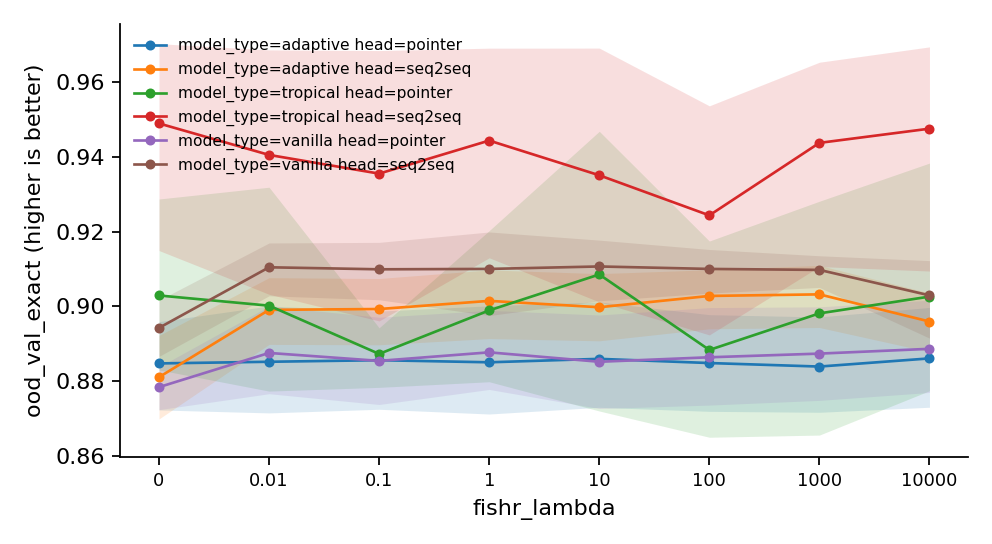
\includegraphics[width=\textwidth]{metric_ood_val_exact.png}
\caption{\texttt{ood\_val\_exact} against \texttt{fishr\_lambda}: the mean over seeds with a 95\% bootstrap CI, one line per combination of the other factors.}
\label{fig:ood_val_exact}
\end{figure}

{\small
\begin{longtable}{lllrlrrr}
\caption{\texttt{ood\_val\_exact} per cell: mean, 95\% bootstrap CI, SD, seeds, diverged runs.}\label{tab:summary-ood_val_exact}\\
\toprule
\texttt{model\_type} & \texttt{head} & \texttt{fishr\_lambda} & mean & 95\% CI & SD & $n$ & div.\\
\midrule
\endhead
adaptive & pointer & 0 & 0.8848 & [0.872, 0.896] & 0.0154 & 5 & 0\\
adaptive & pointer & 0.01 & 0.8852 & [0.872, 0.9] & 0.0187 & 5 & 0\\
adaptive & pointer & 0.1 & 0.8856 & [0.873, 0.899] & 0.0174 & 5 & 0\\
adaptive & pointer & 1 & 0.8851 & [0.871, 0.9] & 0.0203 & 5 & 0\\
adaptive & pointer & 10 & 0.886 & [0.873, 0.901] & 0.0172 & 5 & 0\\
adaptive & pointer & 100 & 0.8849 & [0.872, 0.898] & 0.0173 & 5 & 0\\
adaptive & pointer & 1000 & 0.8839 & [0.872, 0.897] & 0.0163 & 5 & 0\\
adaptive & pointer & 1e+04 & 0.8861 & [0.873, 0.9] & 0.0173 & 5 & 0\\
adaptive & seq2seq & 0 & 0.8811 & [0.87, 0.892] & 0.0148 & 5 & 0\\
adaptive & seq2seq & 0.01 & 0.8991 & [0.89, 0.908] & 0.0119 & 5 & 0\\
adaptive & seq2seq & 0.1 & 0.8993 & [0.89, 0.907] & 0.0115 & 5 & 0\\
adaptive & seq2seq & 1 & 0.9015 & [0.891, 0.91] & 0.0116 & 5 & 0\\
adaptive & seq2seq & 10 & 0.8998 & [0.891, 0.909] & 0.0116 & 5 & 0\\
adaptive & seq2seq & 100 & 0.9028 & [0.894, 0.91] & 0.0112 & 5 & 0\\
adaptive & seq2seq & 1000 & 0.9032 & [0.894, 0.911] & 0.0105 & 5 & 0\\
adaptive & seq2seq & 1e+04 & 0.896 & [0.888, 0.904] & 0.0107 & 5 & 0\\
tropical & pointer & 0 & 0.9029 & [0.883, 0.929] & 0.029 & 5 & 0\\
tropical & pointer & 0.01 & 0.9002 & [0.877, 0.932] & 0.0366 & 5 & 0\\
tropical & pointer & 0.1 & 0.8873 & [0.878, 0.894] & 0.0102 & 5 & 0\\
tropical & pointer & 1 & 0.899 & [0.88, 0.92] & 0.0256 & 5 & 0\\
tropical & pointer & 10 & 0.9086 & [0.872, 0.947] & 0.048 & 5 & 0\\
tropical & pointer & 100 & 0.8884 & [0.865, 0.918] & 0.0323 & 5 & 0\\
tropical & pointer & 1000 & 0.8982 & [0.866, 0.928] & 0.042 & 5 & 0\\
tropical & pointer & 1e+04 & 0.9026 & [0.877, 0.938] & 0.0402 & 5 & 0\\
tropical & seq2seq & 0 & 0.9489 & [0.915, 0.97] & 0.0369 & 5 & 0\\
tropical & seq2seq & 0.01 & 0.9405 & [0.903, 0.969] & 0.0418 & 5 & 0\\
tropical & seq2seq & 0.1 & 0.9355 & [0.896, 0.968] & 0.0462 & 5 & 0\\
tropical & seq2seq & 1 & 0.9444 & [0.913, 0.969] & 0.0367 & 5 & 0\\
tropical & seq2seq & 10 & 0.9351 & [0.901, 0.969] & 0.0458 & 5 & 0\\
tropical & seq2seq & 100 & 0.9244 & [0.892, 0.954] & 0.0407 & 5 & 0\\
tropical & seq2seq & 1000 & 0.9437 & [0.911, 0.965] & 0.0364 & 5 & 0\\
tropical & seq2seq & 1e+04 & 0.9475 & [0.909, 0.969] & 0.042 & 5 & 0\\
vanilla & pointer & 0 & 0.8784 & [0.872, 0.884] & 0.00747 & 5 & 0\\
vanilla & pointer & 0.01 & 0.8876 & [0.877, 0.9] & 0.0154 & 5 & 0\\
vanilla & pointer & 0.1 & 0.8855 & [0.874, 0.897] & 0.0156 & 5 & 0\\
vanilla & pointer & 1 & 0.8877 & [0.878, 0.899] & 0.0137 & 5 & 0\\
vanilla & pointer & 10 & 0.8852 & [0.873, 0.898] & 0.0168 & 5 & 0\\
vanilla & pointer & 100 & 0.8864 & [0.874, 0.9] & 0.0166 & 5 & 0\\
vanilla & pointer & 1000 & 0.8874 & [0.875, 0.9] & 0.0167 & 5 & 0\\
vanilla & pointer & 1e+04 & 0.8887 & [0.877, 0.902] & 0.0158 & 5 & 0\\
vanilla & seq2seq & 0 & 0.8943 & [0.887, 0.902] & 0.00983 & 5 & 0\\
vanilla & seq2seq & 0.01 & 0.9105 & [0.903, 0.917] & 0.00883 & 5 & 0\\
vanilla & seq2seq & 0.1 & 0.9099 & [0.902, 0.917] & 0.00928 & 5 & 0\\
vanilla & seq2seq & 1 & 0.91 & [0.898, 0.92] & 0.0147 & 5 & 0\\
vanilla & seq2seq & 10 & 0.9107 & [0.902, 0.918] & 0.0105 & 5 & 0\\
vanilla & seq2seq & 100 & 0.91 & [0.904, 0.915] & 0.00784 & 5 & 0\\
vanilla & seq2seq & 1000 & 0.9098 & [0.905, 0.914] & 0.00538 & 5 & 0\\
vanilla & seq2seq & 1e+04 & 0.903 & [0.892, 0.912] & 0.0138 & 5 & 0\\
\bottomrule
\end{longtable}
}

{\small
\begin{longtable}{lllrrrl}
\caption{\texttt{ood\_val\_exact}: each level of \texttt{fishr\_lambda} against its control (0), within each combination of the other factors. parametric: Dunnett vs control.}\label{tab:control-ood_val_exact}\\
\toprule
\texttt{model\_type} & \texttt{head} & \texttt{fishr\_lambda} & difference & 95\% CI & $p$ & \\
\midrule
\endhead
adaptive & pointer & 0.01 & $4.400\times10^{-4}$ & [-0.0302, 0.0311] & 1.0000 & \\
adaptive & pointer & 0.1 & $8.600\times10^{-4}$ & [-0.0298, 0.0315] & 1.0000 & \\
adaptive & pointer & 1 & $3.000\times10^{-4}$ & [-0.0303, 0.0309] & 1.0000 & \\
adaptive & pointer & 10 & 0.00122 & [-0.0294, 0.0319] & 1.0000 & \\
adaptive & pointer & 100 & $1.000\times10^{-4}$ & [-0.0305, 0.0307] & 1.0000 & \\
adaptive & pointer & 1000 & $-8.400\times10^{-4}$ & [-0.0315, 0.0298] & 1.0000 & \\
adaptive & pointer & 1e+04 & 0.00134 & [-0.0293, 0.032] & 1.0000 & \\
adaptive & seq2seq & 0.01 & 0.018 & [-0.00265, 0.0386] & 0.1081 & \\
adaptive & seq2seq & 0.1 & 0.01822 & [-0.00243, 0.0389] & 0.1015 & \\
adaptive & seq2seq & 1 & 0.0204 & [$-2.48\times10^{-4}$, 0.041] & 0.0539 & \\
adaptive & seq2seq & 10 & 0.0187 & [-0.00195, 0.0393] & 0.0889 & \\
adaptive & seq2seq & 100 & 0.02172 & [0.00107, 0.0424] & 0.0358 & *\\
adaptive & seq2seq & 1000 & 0.02214 & [0.00149, 0.0428] & 0.0314 & *\\
adaptive & seq2seq & 1e+04 & 0.01488 & [-0.00577, 0.0355] & 0.2414 & \\
tropical & pointer & 0.01 & -0.00272 & [-0.0634, 0.058] & 1.0000 & \\
tropical & pointer & 0.1 & -0.01562 & [-0.0763, 0.0451] & 0.9680 & \\
tropical & pointer & 1 & -0.00398 & [-0.0647, 0.0567] & 1.0000 & \\
tropical & pointer & 10 & 0.00562 & [-0.0551, 0.0663] & 0.9999 & \\
tropical & pointer & 100 & -0.01456 & [-0.0753, 0.0462] & 0.9777 & \\
tropical & pointer & 1000 & -0.00478 & [-0.0655, 0.0559] & 1.0000 & \\
tropical & pointer & 1e+04 & $-3.000\times10^{-4}$ & [-0.061, 0.0604] & 1.0000 & \\
tropical & seq2seq & 0.01 & -0.00842 & [-0.08, 0.0632] & 0.9997 & \\
tropical & seq2seq & 0.1 & -0.01342 & [-0.085, 0.0582] & 0.9943 & \\
tropical & seq2seq & 1 & -0.00458 & [-0.0762, 0.067] & 1.0000 & \\
tropical & seq2seq & 10 & -0.01386 & [-0.0854, 0.0577] & 0.9931 & \\
tropical & seq2seq & 100 & -0.02458 & [-0.0962, 0.047] & 0.8815 & \\
tropical & seq2seq & 1000 & -0.0052 & [-0.0768, 0.0664] & 1.0000 & \\
tropical & seq2seq & 1e+04 & -0.0014 & [-0.073, 0.0702] & 1.0000 & \\
vanilla & pointer & 0.01 & 0.00914 & [-0.0171, 0.0354] & 0.8753 & \\
vanilla & pointer & 0.1 & 0.00702 & [-0.0193, 0.0333] & 0.9614 & \\
vanilla & pointer & 1 & 0.0093 & [-0.017, 0.0356] & 0.8666 & \\
vanilla & pointer & 10 & 0.00678 & [-0.0195, 0.0331] & 0.9675 & \\
vanilla & pointer & 100 & 0.00798 & [-0.0183, 0.0343] & 0.9296 & \\
vanilla & pointer & 1000 & 0.00896 & [-0.0173, 0.0352] & 0.8848 & \\
vanilla & pointer & 1e+04 & 0.01024 & [-0.016, 0.0365] & 0.8098 & \\
vanilla & seq2seq & 0.01 & 0.0162 & [-0.00196, 0.0344] & 0.0960 & \\
vanilla & seq2seq & 0.1 & 0.01566 & [-0.0025, 0.0338] & 0.1138 & \\
vanilla & seq2seq & 1 & 0.01576 & [-0.0024, 0.0339] & 0.1104 & \\
vanilla & seq2seq & 10 & 0.01642 & [-0.00174, 0.0346] & 0.0895 & \\
vanilla & seq2seq & 100 & 0.01576 & [-0.0024, 0.0339] & 0.1105 & \\
vanilla & seq2seq & 1000 & 0.0155 & [-0.00266, 0.0337] & 0.1197 & \\
vanilla & seq2seq & 1e+04 & 0.0087 & [-0.00946, 0.0269] & 0.6422 & \\
\bottomrule
\end{longtable}
}

{\small
\begin{longtable}{llrrrrr}
\caption{\texttt{ood\_val\_exact} against log10 \texttt{fishr\_lambda}: parametric: OLS slope t-test, seed-bootstrap CI, with the Jonckheere--Terpstra ordered-trend $\tau$ and $p$.}\label{tab:trend-ood_val_exact}\\
\toprule
\texttt{model\_type} & \texttt{head} & estimate & 95\% CI & $p$ & JT $\tau$ & JT $p$\\
\midrule
\endhead
adaptive & pointer & $-3.214\times10^{-5}$ & [$-2.82\times10^{-4}$, $2.11\times10^{-4}$] & 0.9817 & 0.00762 & 0.9634\\
adaptive & seq2seq & $-7.143\times10^{-6}$ & [$-6.06\times10^{-4}$, $8.13\times10^{-4}$] & 0.9937 & 0.0152 & 0.9182\\
tropical & pointer & $6.557\times10^{-4}$ & [-0.00179, 0.00265] & 0.8181 & 0.0457 & 0.7419\\
tropical & seq2seq & $6.250\times10^{-4}$ & [-0.00205, 0.00291] & 0.8506 & 0.04 & 0.7690\\
vanilla & pointer & $2.093\times10^{-4}$ & [$-5.57\times10^{-5}$, $4.35\times10^{-4}$] & 0.8666 & 0.0381 & 0.7806\\
vanilla & seq2seq & $-8.150\times10^{-4}$ & [-0.00118, $-4.05\times10^{-4}$] & 0.3347 & -0.107 & 0.4189\\
\bottomrule
\end{longtable}
}

{\small
\begin{longtable}{lrrrl}
\caption{\texttt{ood\_val\_exact}: paired contrasts by seed, Holm-corrected across the cells. parametric: paired t-test by seed, Holm.}\label{tab:paired-ood_val_exact}\\
\toprule
contrast (within) & difference & 95\% CI & $p$ & \\
\midrule
\endhead
\stackcell{model\_type: tropical - vanilla\\\footnotesize head=pointer fishr\_lambda=0 } & 0.0245 & [-0.0168, 0.0658] & 1.0000 & \\
\stackcell{model\_type: tropical - vanilla\\\footnotesize head=pointer fishr\_lambda=0.01 } & 0.01264 & [-0.0176, 0.0428] & 1.0000 & \\
\stackcell{model\_type: tropical - vanilla\\\footnotesize head=pointer fishr\_lambda=0.1 } & 0.00186 & [-0.0129, 0.0166] & 1.0000 & \\
\stackcell{model\_type: tropical - vanilla\\\footnotesize head=pointer fishr\_lambda=1 } & 0.01122 & [-0.0128, 0.0353] & 1.0000 & \\
\stackcell{model\_type: tropical - vanilla\\\footnotesize head=pointer fishr\_lambda=10 } & 0.02334 & [-0.0331, 0.0798] & 1.0000 & \\
\stackcell{model\_type: tropical - vanilla\\\footnotesize head=pointer fishr\_lambda=100 } & 0.00196 & [-0.03, 0.034] & 1.0000 & \\
\stackcell{model\_type: tropical - vanilla\\\footnotesize head=pointer fishr\_lambda=1000 } & 0.01076 & [-0.0315, 0.0531] & 1.0000 & \\
\stackcell{model\_type: tropical - vanilla\\\footnotesize head=pointer fishr\_lambda=1e+04 } & 0.01396 & [-0.0208, 0.0487] & 1.0000 & \\
\stackcell{model\_type: tropical - vanilla\\\footnotesize head=seq2seq fishr\_lambda=0 } & 0.05466 & [0.0179, 0.0914] & 0.2327 & \\
\stackcell{model\_type: tropical - vanilla\\\footnotesize head=seq2seq fishr\_lambda=0.01 } & 0.03004 & [-0.0132, 0.0733] & 1.0000 & \\
\stackcell{model\_type: tropical - vanilla\\\footnotesize head=seq2seq fishr\_lambda=0.1 } & 0.02558 & [-0.0284, 0.0796] & 1.0000 & \\
\stackcell{model\_type: tropical - vanilla\\\footnotesize head=seq2seq fishr\_lambda=1 } & 0.03432 & [0.00284, 0.0658] & 0.5448 & \\
\stackcell{model\_type: tropical - vanilla\\\footnotesize head=seq2seq fishr\_lambda=10 } & 0.02438 & [-0.0262, 0.075] & 1.0000 & \\
\stackcell{model\_type: tropical - vanilla\\\footnotesize head=seq2seq fishr\_lambda=100 } & 0.01432 & [-0.0305, 0.0591] & 1.0000 & \\
\stackcell{model\_type: tropical - vanilla\\\footnotesize head=seq2seq fishr\_lambda=1000 } & 0.03396 & [-0.00548, 0.0734] & 0.9762 & \\
\stackcell{model\_type: tropical - vanilla\\\footnotesize head=seq2seq fishr\_lambda=1e+04 } & 0.04456 & [0.0083, 0.0808] & 0.4047 & \\
\stackcell{model\_type: adaptive - vanilla\\\footnotesize head=pointer fishr\_lambda=0 } & 0.00634 & [-0.00733, 0.02] & 1.0000 & \\
\stackcell{model\_type: adaptive - vanilla\\\footnotesize head=pointer fishr\_lambda=0.01 } & -0.00236 & [-0.0124, 0.00765] & 1.0000 & \\
\stackcell{model\_type: adaptive - vanilla\\\footnotesize head=pointer fishr\_lambda=0.1 } & $1.800\times10^{-4}$ & [-0.00626, 0.00662] & 1.0000 & \\
\stackcell{model\_type: adaptive - vanilla\\\footnotesize head=pointer fishr\_lambda=1 } & -0.00266 & [-0.0126, 0.00727] & 1.0000 & \\
\stackcell{model\_type: adaptive - vanilla\\\footnotesize head=pointer fishr\_lambda=10 } & $7.800\times10^{-4}$ & [-0.00538, 0.00694] & 1.0000 & \\
\stackcell{model\_type: adaptive - vanilla\\\footnotesize head=pointer fishr\_lambda=100 } & -0.00154 & [-0.00881, 0.00573] & 1.0000 & \\
\stackcell{model\_type: adaptive - vanilla\\\footnotesize head=pointer fishr\_lambda=1000 } & -0.00346 & [-0.00884, 0.00192] & 1.0000 & \\
\stackcell{model\_type: adaptive - vanilla\\\footnotesize head=pointer fishr\_lambda=1e+04 } & -0.00256 & [-0.0113, 0.00622] & 1.0000 & \\
\stackcell{model\_type: adaptive - vanilla\\\footnotesize head=seq2seq fishr\_lambda=0 } & -0.01318 & [-0.0337, 0.00732] & 1.0000 & \\
\stackcell{model\_type: adaptive - vanilla\\\footnotesize head=seq2seq fishr\_lambda=0.01 } & -0.01138 & [-0.0207, -0.0021] & 0.4077 & \\
\stackcell{model\_type: adaptive - vanilla\\\footnotesize head=seq2seq fishr\_lambda=0.1 } & -0.01062 & [-0.0174, -0.00388] & 0.1908 & \\
\stackcell{model\_type: adaptive - vanilla\\\footnotesize head=seq2seq fishr\_lambda=1 } & -0.00854 & [-0.0168, $-2.64\times10^{-4}$] & 0.5941 & \\
\stackcell{model\_type: adaptive - vanilla\\\footnotesize head=seq2seq fishr\_lambda=10 } & -0.0109 & [-0.0202, -0.00156] & 0.4439 & \\
\stackcell{model\_type: adaptive - vanilla\\\footnotesize head=seq2seq fishr\_lambda=100 } & -0.00722 & [-0.0157, 0.00127] & 0.9316 & \\
\stackcell{model\_type: adaptive - vanilla\\\footnotesize head=seq2seq fishr\_lambda=1000 } & -0.00654 & [-0.0161, 0.003] & 1.0000 & \\
\stackcell{model\_type: adaptive - vanilla\\\footnotesize head=seq2seq fishr\_lambda=1e+04 } & -0.007 & [-0.0261, 0.0121] & 1.0000 & \\
\stackcell{head: pointer - seq2seq\\\footnotesize model\_type=adaptive fishr\_lambda=0 } & 0.00368 & [-0.0155, 0.0229] & 0.9298 & \\
\stackcell{head: pointer - seq2seq\\\footnotesize model\_type=adaptive fishr\_lambda=0.01 } & -0.01388 & [-0.0358, 0.00803] & 0.9298 & \\
\stackcell{head: pointer - seq2seq\\\footnotesize model\_type=adaptive fishr\_lambda=0.1 } & -0.01368 & [-0.0337, 0.00637] & 0.9298 & \\
\stackcell{head: pointer - seq2seq\\\footnotesize model\_type=adaptive fishr\_lambda=1 } & -0.01642 & [-0.0373, 0.00444] & 0.9298 & \\
\stackcell{head: pointer - seq2seq\\\footnotesize model\_type=adaptive fishr\_lambda=10 } & -0.0138 & [-0.0367, 0.00912] & 0.9298 & \\
\stackcell{head: pointer - seq2seq\\\footnotesize model\_type=adaptive fishr\_lambda=100 } & -0.01794 & [-0.0323, -0.00355] & 0.5296 & \\
\stackcell{head: pointer - seq2seq\\\footnotesize model\_type=adaptive fishr\_lambda=1000 } & -0.0193 & [-0.0364, -0.00218] & 0.6329 & \\
\stackcell{head: pointer - seq2seq\\\footnotesize model\_type=adaptive fishr\_lambda=1e+04 } & -0.00986 & [-0.0371, 0.0174] & 0.9298 & \\
\stackcell{head: pointer - seq2seq\\\footnotesize model\_type=tropical fishr\_lambda=0 } & -0.046 & [-0.117, 0.0249] & 0.9298 & \\
\stackcell{head: pointer - seq2seq\\\footnotesize model\_type=tropical fishr\_lambda=0.01 } & -0.0403 & [-0.0826, 0.00199] & 0.6866 & \\
\stackcell{head: pointer - seq2seq\\\footnotesize model\_type=tropical fishr\_lambda=0.1 } & -0.0482 & [-0.107, 0.0104] & 0.9298 & \\
\stackcell{head: pointer - seq2seq\\\footnotesize model\_type=tropical fishr\_lambda=1 } & -0.0454 & [-0.0748, -0.016] & 0.2814 & \\
\stackcell{head: pointer - seq2seq\\\footnotesize model\_type=tropical fishr\_lambda=10 } & -0.02652 & [-0.0631, 0.0101] & 0.9298 & \\
\stackcell{head: pointer - seq2seq\\\footnotesize model\_type=tropical fishr\_lambda=100 } & -0.03598 & [-0.0697, -0.00227] & 0.6329 & \\
\stackcell{head: pointer - seq2seq\\\footnotesize model\_type=tropical fishr\_lambda=1000 } & -0.04558 & [-0.0706, -0.0205] & 0.1738 & \\
\stackcell{head: pointer - seq2seq\\\footnotesize model\_type=tropical fishr\_lambda=1e+04 } & -0.0449 & [-0.1, 0.0102] & 0.9298 & \\
\stackcell{head: pointer - seq2seq\\\footnotesize model\_type=vanilla fishr\_lambda=0 } & -0.01584 & [-0.0253, -0.00634] & 0.2260 & \\
\stackcell{head: pointer - seq2seq\\\footnotesize model\_type=vanilla fishr\_lambda=0.01 } & -0.0229 & [-0.044, -0.00177] & 0.6329 & \\
\stackcell{head: pointer - seq2seq\\\footnotesize model\_type=vanilla fishr\_lambda=0.1 } & -0.02448 & [-0.044, -0.00498] & 0.5296 & \\
\stackcell{head: pointer - seq2seq\\\footnotesize model\_type=vanilla fishr\_lambda=1 } & -0.0223 & [-0.0446, $8.87\times10^{-6}$] & 0.6507 & \\
\stackcell{head: pointer - seq2seq\\\footnotesize model\_type=vanilla fishr\_lambda=10 } & -0.02548 & [-0.0466, -0.0044] & 0.5394 & \\
\stackcell{head: pointer - seq2seq\\\footnotesize model\_type=vanilla fishr\_lambda=100 } & -0.02362 & [-0.0446, -0.00262] & 0.6329 & \\
\stackcell{head: pointer - seq2seq\\\footnotesize model\_type=vanilla fishr\_lambda=1000 } & -0.02238 & [-0.0424, -0.00241] & 0.6329 & \\
\stackcell{head: pointer - seq2seq\\\footnotesize model\_type=vanilla fishr\_lambda=1e+04 } & -0.0143 & [-0.0396, 0.011] & 0.9298 & \\
\bottomrule
\end{longtable}
}

\subsection{\texttt{ood\_noise\_f1}}
\begin{figure}[tbp]
\centering
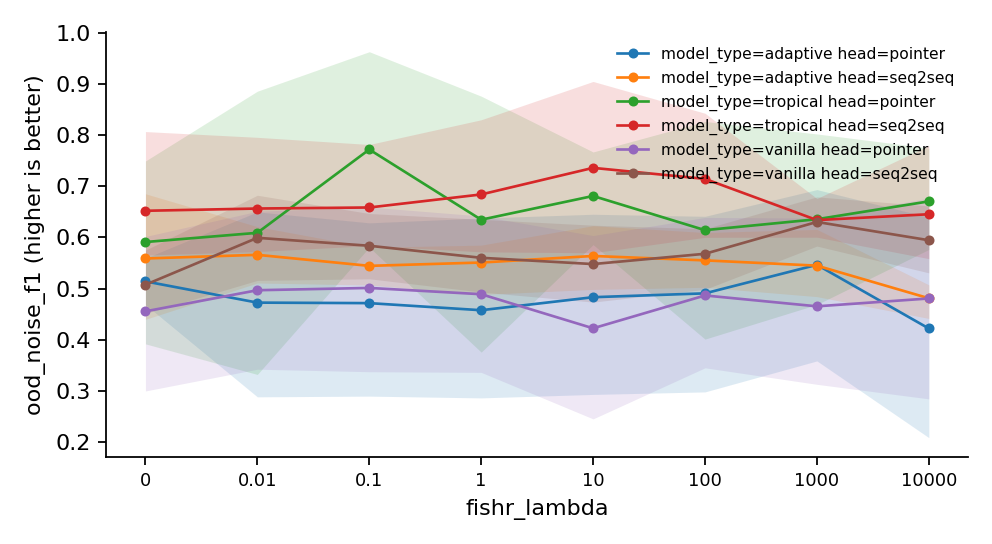
\includegraphics[width=\textwidth]{metric_ood_noise_f1.png}
\caption{\texttt{ood\_noise\_f1} against \texttt{fishr\_lambda}: the mean over seeds with a 95\% bootstrap CI, one line per combination of the other factors.}
\label{fig:ood_noise_f1}
\end{figure}

{\small
\begin{longtable}{lllrlrrr}
\caption{\texttt{ood\_noise\_f1} per cell: mean, 95\% bootstrap CI, SD, seeds, diverged runs.}\label{tab:summary-ood_noise_f1}\\
\toprule
\texttt{model\_type} & \texttt{head} & \texttt{fishr\_lambda} & mean & 95\% CI & SD & $n$ & div.\\
\midrule
\endhead
adaptive & pointer & 0 & 0.514 & [0.469, 0.559] & 0.0594 & 5 & 0\\
adaptive & pointer & 0.01 & 0.4725 & [0.288, 0.65] & 0.235 & 5 & 0\\
adaptive & pointer & 0.1 & 0.4715 & [0.29, 0.629] & 0.22 & 5 & 0\\
adaptive & pointer & 1 & 0.4577 & [0.286, 0.638] & 0.216 & 5 & 0\\
adaptive & pointer & 10 & 0.4831 & [0.293, 0.645] & 0.216 & 5 & 0\\
adaptive & pointer & 100 & 0.4907 & [0.298, 0.641] & 0.217 & 5 & 0\\
adaptive & pointer & 1000 & 0.5465 & [0.359, 0.693] & 0.223 & 5 & 0\\
adaptive & pointer & 1e+04 & 0.422 & [0.209, 0.639] & 0.283 & 5 & 0\\
adaptive & seq2seq & 0 & 0.5588 & [0.44, 0.685] & 0.156 & 5 & 0\\
adaptive & seq2seq & 0.01 & 0.566 & [0.511, 0.621] & 0.0702 & 5 & 0\\
adaptive & seq2seq & 0.1 & 0.5444 & [0.507, 0.581] & 0.0455 & 5 & 0\\
adaptive & seq2seq & 1 & 0.5509 & [0.488, 0.585] & 0.0694 & 5 & 0\\
adaptive & seq2seq & 10 & 0.5637 & [0.498, 0.623] & 0.0872 & 5 & 0\\
adaptive & seq2seq & 100 & 0.5551 & [0.503, 0.61] & 0.0709 & 5 & 0\\
adaptive & seq2seq & 1000 & 0.5448 & [0.484, 0.616] & 0.088 & 5 & 0\\
adaptive & seq2seq & 1e+04 & 0.481 & [0.442, 0.507] & 0.0432 & 5 & 0\\
tropical & pointer & 0 & 0.591 & [0.392, 0.749] & 0.239 & 5 & 0\\
tropical & pointer & 0.01 & 0.609 & [0.332, 0.886] & 0.366 & 5 & 0\\
tropical & pointer & 0.1 & 0.7719 & [0.581, 0.963] & 0.244 & 5 & 0\\
tropical & pointer & 1 & 0.6346 & [0.376, 0.876] & 0.327 & 5 & 0\\
tropical & pointer & 10 & 0.681 & [0.586, 0.767] & 0.115 & 5 & 0\\
tropical & pointer & 100 & 0.6142 & [0.401, 0.827] & 0.282 & 5 & 0\\
tropical & pointer & 1000 & 0.6355 & [0.469, 0.802] & 0.217 & 5 & 0\\
tropical & pointer & 1e+04 & 0.6705 & [0.576, 0.775] & 0.129 & 5 & 0\\
tropical & seq2seq & 0 & 0.6521 & [0.566, 0.807] & 0.174 & 5 & 0\\
tropical & seq2seq & 0.01 & 0.6565 & [0.572, 0.796] & 0.155 & 5 & 0\\
tropical & seq2seq & 0.1 & 0.6585 & [0.584, 0.782] & 0.139 & 5 & 0\\
tropical & seq2seq & 1 & 0.684 & [0.572, 0.83] & 0.183 & 5 & 0\\
tropical & seq2seq & 10 & 0.736 & [0.57, 0.905] & 0.22 & 5 & 0\\
tropical & seq2seq & 100 & 0.7144 & [0.6, 0.843] & 0.165 & 5 & 0\\
tropical & seq2seq & 1000 & 0.6339 & [0.6, 0.676] & 0.0458 & 5 & 0\\
tropical & seq2seq & 1e+04 & 0.6453 & [0.558, 0.78] & 0.146 & 5 & 0\\
vanilla & pointer & 0 & 0.4555 & [0.3, 0.602] & 0.196 & 5 & 0\\
vanilla & pointer & 0.01 & 0.4968 & [0.342, 0.651] & 0.198 & 5 & 0\\
vanilla & pointer & 0.1 & 0.5012 & [0.337, 0.659] & 0.209 & 5 & 0\\
vanilla & pointer & 1 & 0.489 & [0.336, 0.642] & 0.198 & 5 & 0\\
vanilla & pointer & 10 & 0.4223 & [0.245, 0.604] & 0.218 & 5 & 0\\
vanilla & pointer & 100 & 0.4865 & [0.345, 0.639] & 0.192 & 5 & 0\\
vanilla & pointer & 1000 & 0.4653 & [0.313, 0.638] & 0.213 & 5 & 0\\
vanilla & pointer & 1e+04 & 0.4806 & [0.284, 0.677] & 0.25 & 5 & 0\\
vanilla & seq2seq & 0 & 0.5075 & [0.451, 0.575] & 0.0823 & 5 & 0\\
vanilla & seq2seq & 0.01 & 0.5992 & [0.516, 0.682] & 0.113 & 5 & 0\\
vanilla & seq2seq & 0.1 & 0.5837 & [0.519, 0.647] & 0.0894 & 5 & 0\\
vanilla & seq2seq & 1 & 0.5601 & [0.493, 0.635] & 0.0883 & 5 & 0\\
vanilla & seq2seq & 10 & 0.5479 & [0.474, 0.624] & 0.0925 & 5 & 0\\
vanilla & seq2seq & 100 & 0.568 & [0.498, 0.617] & 0.0795 & 5 & 0\\
vanilla & seq2seq & 1000 & 0.6303 & [0.583, 0.679] & 0.0657 & 5 & 0\\
vanilla & seq2seq & 1e+04 & 0.5945 & [0.531, 0.662] & 0.0867 & 5 & 0\\
\bottomrule
\end{longtable}
}

{\small
\begin{longtable}{lllrrrl}
\caption{\texttt{ood\_noise\_f1}: each level of \texttt{fishr\_lambda} against its control (0), within each combination of the other factors. parametric: Dunnett vs control.}\label{tab:control-ood_noise_f1}\\
\toprule
\texttt{model\_type} & \texttt{head} & \texttt{fishr\_lambda} & difference & 95\% CI & $p$ & \\
\midrule
\endhead
adaptive & pointer & 0.01 & -0.04148 & [-0.421, 0.338] & 0.9998 & \\
adaptive & pointer & 0.1 & -0.04248 & [-0.422, 0.337] & 0.9998 & \\
adaptive & pointer & 1 & -0.05634 & [-0.436, 0.323] & 0.9986 & \\
adaptive & pointer & 10 & -0.03088 & [-0.41, 0.348] & 1.0000 & \\
adaptive & pointer & 100 & -0.02337 & [-0.403, 0.356] & 1.0000 & \\
adaptive & pointer & 1000 & 0.03244 & [-0.347, 0.412] & 1.0000 & \\
adaptive & pointer & 1e+04 & -0.09205 & [-0.471, 0.287] & 0.9762 & \\
adaptive & seq2seq & 0.01 & 0.00718 & [-0.142, 0.156] & 1.0000 & \\
adaptive & seq2seq & 0.1 & -0.01441 & [-0.164, 0.135] & 0.9999 & \\
adaptive & seq2seq & 1 & -0.007882 & [-0.157, 0.141] & 1.0000 & \\
adaptive & seq2seq & 10 & 0.004937 & [-0.144, 0.154] & 1.0000 & \\
adaptive & seq2seq & 100 & -0.003685 & [-0.153, 0.146] & 1.0000 & \\
adaptive & seq2seq & 1000 & -0.01398 & [-0.163, 0.135] & 0.9999 & \\
adaptive & seq2seq & 1e+04 & -0.07775 & [-0.227, 0.0715] & 0.5607 & \\
tropical & pointer & 0.01 & 0.01799 & [-0.425, 0.461] & 1.0000 & \\
tropical & pointer & 0.1 & 0.1809 & [-0.262, 0.624] & 0.7767 & \\
tropical & pointer & 1 & 0.04363 & [-0.399, 0.486] & 0.9999 & \\
tropical & pointer & 10 & 0.09004 & [-0.353, 0.533] & 0.9909 & \\
tropical & pointer & 100 & 0.0232 & [-0.42, 0.466] & 1.0000 & \\
tropical & pointer & 1000 & 0.04455 & [-0.398, 0.487] & 0.9999 & \\
tropical & pointer & 1e+04 & 0.07948 & [-0.363, 0.522] & 0.9956 & \\
tropical & seq2seq & 0.01 & 0.004421 & [-0.276, 0.285] & 1.0000 & \\
tropical & seq2seq & 0.1 & 0.006455 & [-0.274, 0.287] & 1.0000 & \\
tropical & seq2seq & 1 & 0.03195 & [-0.248, 0.312] & 0.9997 & \\
tropical & seq2seq & 10 & 0.08392 & [-0.196, 0.364] & 0.9339 & \\
tropical & seq2seq & 100 & 0.06238 & [-0.218, 0.343] & 0.9850 & \\
tropical & seq2seq & 1000 & -0.01818 & [-0.298, 0.262] & 1.0000 & \\
tropical & seq2seq & 1e+04 & -0.006761 & [-0.287, 0.273] & 1.0000 & \\
vanilla & pointer & 0.01 & 0.04127 & [-0.326, 0.408] & 0.9998 & \\
vanilla & pointer & 0.1 & 0.04576 & [-0.321, 0.413] & 0.9995 & \\
vanilla & pointer & 1 & 0.03348 & [-0.333, 0.4] & 0.9999 & \\
vanilla & pointer & 10 & -0.03316 & [-0.4, 0.334] & 0.9999 & \\
vanilla & pointer & 100 & 0.03104 & [-0.336, 0.398] & 1.0000 & \\
vanilla & pointer & 1000 & 0.009812 & [-0.357, 0.377] & 1.0000 & \\
vanilla & pointer & 1e+04 & 0.02515 & [-0.342, 0.392] & 1.0000 & \\
vanilla & seq2seq & 0.01 & 0.0917 & [-0.0622, 0.246] & 0.4226 & \\
vanilla & seq2seq & 0.1 & 0.07618 & [-0.0777, 0.23] & 0.6109 & \\
vanilla & seq2seq & 1 & 0.05263 & [-0.101, 0.206] & 0.8834 & \\
vanilla & seq2seq & 10 & 0.04038 & [-0.113, 0.194] & 0.9646 & \\
vanilla & seq2seq & 100 & 0.0605 & [-0.0934, 0.214] & 0.8037 & \\
vanilla & seq2seq & 1000 & 0.1227 & [-0.0311, 0.277] & 0.1627 & \\
vanilla & seq2seq & 1e+04 & 0.087 & [-0.0669, 0.241] & 0.4767 & \\
\bottomrule
\end{longtable}
}

{\small
\begin{longtable}{llrrrrr}
\caption{\texttt{ood\_noise\_f1} against log10 \texttt{fishr\_lambda}: parametric: OLS slope t-test, seed-bootstrap CI, with the Jonckheere--Terpstra ordered-trend $\tau$ and $p$.}\label{tab:trend-ood_noise_f1}\\
\toprule
\texttt{model\_type} & \texttt{head} & estimate & 95\% CI & $p$ & JT $\tau$ & JT $p$\\
\midrule
\endhead
adaptive & pointer & 0.001111 & [-0.0117, 0.0125] & 0.9518 & 0.0895 & 0.5175\\
adaptive & seq2seq & -0.00892 & [-0.0194, 0.00125] & 0.1271 & -0.204 & 0.1290\\
tropical & pointer & -0.003882 & [-0.043, 0.0385] & 0.8502 & -0.0705 & 0.6019\\
tropical & seq2seq & -0.001871 & [-0.011, 0.00384] & 0.8838 & 0.0514 & 0.7161\\
vanilla & pointer & -0.004381 & [-0.0165, 0.00469] & 0.7938 & -0.059 & 0.6565\\
vanilla & seq2seq & 0.003103 & [-0.0142, 0.0225] & 0.6714 & 0.0552 & 0.6961\\
\bottomrule
\end{longtable}
}

{\small
\begin{longtable}{lrrrl}
\caption{\texttt{ood\_noise\_f1}: paired contrasts by seed, Holm-corrected across the cells. parametric: paired t-test by seed, Holm.}\label{tab:paired-ood_noise_f1}\\
\toprule
contrast (within) & difference & 95\% CI & $p$ & \\
\midrule
\endhead
\stackcell{model\_type: tropical - vanilla\\\footnotesize head=pointer fishr\_lambda=0 } & 0.1355 & [-0.303, 0.574] & 1.0000 & \\
\stackcell{model\_type: tropical - vanilla\\\footnotesize head=pointer fishr\_lambda=0.01 } & 0.1122 & [-0.353, 0.577] & 1.0000 & \\
\stackcell{model\_type: tropical - vanilla\\\footnotesize head=pointer fishr\_lambda=0.1 } & 0.2707 & [-0.0843, 0.626] & 1.0000 & \\
\stackcell{model\_type: tropical - vanilla\\\footnotesize head=pointer fishr\_lambda=1 } & 0.1457 & [-0.246, 0.538] & 1.0000 & \\
\stackcell{model\_type: tropical - vanilla\\\footnotesize head=pointer fishr\_lambda=10 } & 0.2587 & [-0.0612, 0.579] & 1.0000 & \\
\stackcell{model\_type: tropical - vanilla\\\footnotesize head=pointer fishr\_lambda=100 } & 0.1277 & [-0.382, 0.637] & 1.0000 & \\
\stackcell{model\_type: tropical - vanilla\\\footnotesize head=pointer fishr\_lambda=1000 } & 0.1702 & [-0.0904, 0.431] & 1.0000 & \\
\stackcell{model\_type: tropical - vanilla\\\footnotesize head=pointer fishr\_lambda=1e+04 } & 0.1898 & [-0.202, 0.582] & 1.0000 & \\
\stackcell{model\_type: tropical - vanilla\\\footnotesize head=seq2seq fishr\_lambda=0 } & 0.1445 & [-0.11, 0.4] & 1.0000 & \\
\stackcell{model\_type: tropical - vanilla\\\footnotesize head=seq2seq fishr\_lambda=0.01 } & 0.05726 & [-0.0888, 0.203] & 1.0000 & \\
\stackcell{model\_type: tropical - vanilla\\\footnotesize head=seq2seq fishr\_lambda=0.1 } & 0.07482 & [-0.115, 0.264] & 1.0000 & \\
\stackcell{model\_type: tropical - vanilla\\\footnotesize head=seq2seq fishr\_lambda=1 } & 0.1239 & [-0.107, 0.354] & 1.0000 & \\
\stackcell{model\_type: tropical - vanilla\\\footnotesize head=seq2seq fishr\_lambda=10 } & 0.1881 & [-0.0402, 0.416] & 1.0000 & \\
\stackcell{model\_type: tropical - vanilla\\\footnotesize head=seq2seq fishr\_lambda=100 } & 0.1464 & [-0.00915, 0.302] & 0.9476 & \\
\stackcell{model\_type: tropical - vanilla\\\footnotesize head=seq2seq fishr\_lambda=1000 } & 0.003626 & [-0.0557, 0.063] & 1.0000 & \\
\stackcell{model\_type: tropical - vanilla\\\footnotesize head=seq2seq fishr\_lambda=1e+04 } & 0.05078 & [-0.203, 0.304] & 1.0000 & \\
\stackcell{model\_type: adaptive - vanilla\\\footnotesize head=pointer fishr\_lambda=0 } & 0.05853 & [-0.217, 0.334] & 1.0000 & \\
\stackcell{model\_type: adaptive - vanilla\\\footnotesize head=pointer fishr\_lambda=0.01 } & -0.02422 & [-0.305, 0.257] & 1.0000 & \\
\stackcell{model\_type: adaptive - vanilla\\\footnotesize head=pointer fishr\_lambda=0.1 } & -0.02971 & [-0.372, 0.313] & 1.0000 & \\
\stackcell{model\_type: adaptive - vanilla\\\footnotesize head=pointer fishr\_lambda=1 } & -0.0313 & [-0.297, 0.234] & 1.0000 & \\
\stackcell{model\_type: adaptive - vanilla\\\footnotesize head=pointer fishr\_lambda=10 } & 0.06081 & [-0.248, 0.37] & 1.0000 & \\
\stackcell{model\_type: adaptive - vanilla\\\footnotesize head=pointer fishr\_lambda=100 } & 0.004116 & [-0.243, 0.252] & 1.0000 & \\
\stackcell{model\_type: adaptive - vanilla\\\footnotesize head=pointer fishr\_lambda=1000 } & 0.08116 & [-0.199, 0.361] & 1.0000 & \\
\stackcell{model\_type: adaptive - vanilla\\\footnotesize head=pointer fishr\_lambda=1e+04 } & -0.05868 & [-0.544, 0.427] & 1.0000 & \\
\stackcell{model\_type: adaptive - vanilla\\\footnotesize head=seq2seq fishr\_lambda=0 } & 0.05128 & [-0.178, 0.281] & 1.0000 & \\
\stackcell{model\_type: adaptive - vanilla\\\footnotesize head=seq2seq fishr\_lambda=0.01 } & -0.03324 & [-0.241, 0.175] & 1.0000 & \\
\stackcell{model\_type: adaptive - vanilla\\\footnotesize head=seq2seq fishr\_lambda=0.1 } & -0.03931 & [-0.183, 0.105] & 1.0000 & \\
\stackcell{model\_type: adaptive - vanilla\\\footnotesize head=seq2seq fishr\_lambda=1 } & -0.009235 & [-0.15, 0.131] & 1.0000 & \\
\stackcell{model\_type: adaptive - vanilla\\\footnotesize head=seq2seq fishr\_lambda=10 } & 0.01584 & [-0.161, 0.193] & 1.0000 & \\
\stackcell{model\_type: adaptive - vanilla\\\footnotesize head=seq2seq fishr\_lambda=100 } & -0.0129 & [-0.153, 0.128] & 1.0000 & \\
\stackcell{model\_type: adaptive - vanilla\\\footnotesize head=seq2seq fishr\_lambda=1000 } & -0.08544 & [-0.26, 0.0888] & 1.0000 & \\
\stackcell{model\_type: adaptive - vanilla\\\footnotesize head=seq2seq fishr\_lambda=1e+04 } & -0.1135 & [-0.26, 0.0329] & 1.0000 & \\
\stackcell{head: pointer - seq2seq\\\footnotesize model\_type=adaptive fishr\_lambda=0 } & -0.04477 & [-0.228, 0.138] & 1.0000 & \\
\stackcell{head: pointer - seq2seq\\\footnotesize model\_type=adaptive fishr\_lambda=0.01 } & -0.09344 & [-0.435, 0.248] & 1.0000 & \\
\stackcell{head: pointer - seq2seq\\\footnotesize model\_type=adaptive fishr\_lambda=0.1 } & -0.07285 & [-0.337, 0.192] & 1.0000 & \\
\stackcell{head: pointer - seq2seq\\\footnotesize model\_type=adaptive fishr\_lambda=1 } & -0.09323 & [-0.383, 0.196] & 1.0000 & \\
\stackcell{head: pointer - seq2seq\\\footnotesize model\_type=adaptive fishr\_lambda=10 } & -0.08059 & [-0.395, 0.234] & 1.0000 & \\
\stackcell{head: pointer - seq2seq\\\footnotesize model\_type=adaptive fishr\_lambda=100 } & -0.06446 & [-0.364, 0.235] & 1.0000 & \\
\stackcell{head: pointer - seq2seq\\\footnotesize model\_type=adaptive fishr\_lambda=1000 } & 0.00165 & [-0.237, 0.24] & 1.0000 & \\
\stackcell{head: pointer - seq2seq\\\footnotesize model\_type=adaptive fishr\_lambda=1e+04 } & -0.05907 & [-0.395, 0.277] & 1.0000 & \\
\stackcell{head: pointer - seq2seq\\\footnotesize model\_type=tropical fishr\_lambda=0 } & -0.06106 & [-0.359, 0.237] & 1.0000 & \\
\stackcell{head: pointer - seq2seq\\\footnotesize model\_type=tropical fishr\_lambda=0.01 } & -0.04749 & [-0.585, 0.49] & 1.0000 & \\
\stackcell{head: pointer - seq2seq\\\footnotesize model\_type=tropical fishr\_lambda=0.1 } & 0.1134 & [-0.129, 0.356] & 1.0000 & \\
\stackcell{head: pointer - seq2seq\\\footnotesize model\_type=tropical fishr\_lambda=1 } & -0.04938 & [-0.639, 0.54] & 1.0000 & \\
\stackcell{head: pointer - seq2seq\\\footnotesize model\_type=tropical fishr\_lambda=10 } & -0.05494 & [-0.298, 0.189] & 1.0000 & \\
\stackcell{head: pointer - seq2seq\\\footnotesize model\_type=tropical fishr\_lambda=100 } & -0.1002 & [-0.651, 0.451] & 1.0000 & \\
\stackcell{head: pointer - seq2seq\\\footnotesize model\_type=tropical fishr\_lambda=1000 } & 0.001671 & [-0.301, 0.304] & 1.0000 & \\
\stackcell{head: pointer - seq2seq\\\footnotesize model\_type=tropical fishr\_lambda=1e+04 } & 0.02518 & [-0.166, 0.217] & 1.0000 & \\
\stackcell{head: pointer - seq2seq\\\footnotesize model\_type=vanilla fishr\_lambda=0 } & -0.05202 & [-0.352, 0.248] & 1.0000 & \\
\stackcell{head: pointer - seq2seq\\\footnotesize model\_type=vanilla fishr\_lambda=0.01 } & -0.1025 & [-0.335, 0.13] & 1.0000 & \\
\stackcell{head: pointer - seq2seq\\\footnotesize model\_type=vanilla fishr\_lambda=0.1 } & -0.08244 & [-0.303, 0.138] & 1.0000 & \\
\stackcell{head: pointer - seq2seq\\\footnotesize model\_type=vanilla fishr\_lambda=1 } & -0.07117 & [-0.26, 0.118] & 1.0000 & \\
\stackcell{head: pointer - seq2seq\\\footnotesize model\_type=vanilla fishr\_lambda=10 } & -0.1256 & [-0.355, 0.104] & 1.0000 & \\
\stackcell{head: pointer - seq2seq\\\footnotesize model\_type=vanilla fishr\_lambda=100 } & -0.08148 & [-0.276, 0.113] & 1.0000 & \\
\stackcell{head: pointer - seq2seq\\\footnotesize model\_type=vanilla fishr\_lambda=1000 } & -0.1649 & [-0.469, 0.139] & 1.0000 & \\
\stackcell{head: pointer - seq2seq\\\footnotesize model\_type=vanilla fishr\_lambda=1e+04 } & -0.1139 & [-0.475, 0.247] & 1.0000 & \\
\bottomrule
\end{longtable}
}

\subsection{\texttt{ood\_noise\_exact}}
\begin{figure}[tbp]
\centering
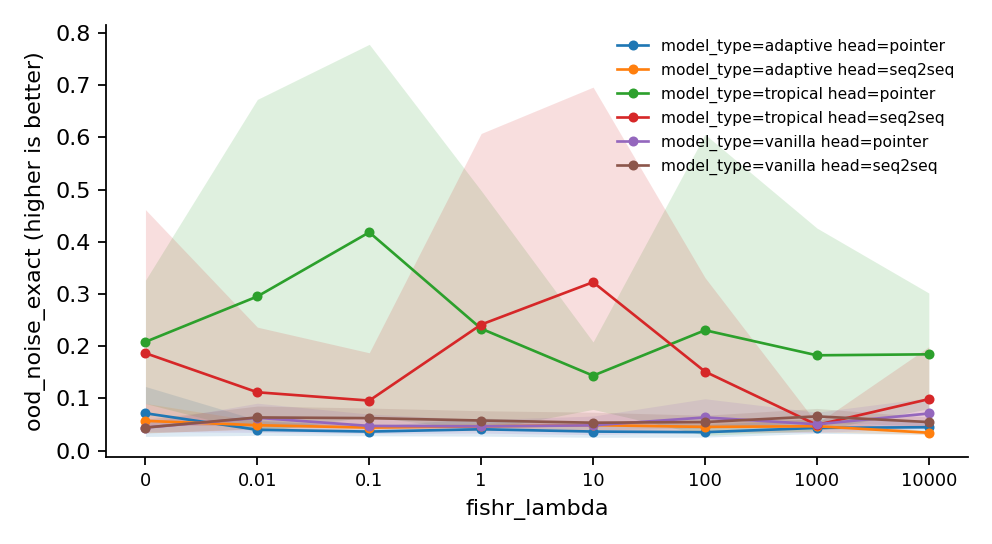
\includegraphics[width=\textwidth]{metric_ood_noise_exact.png}
\caption{\texttt{ood\_noise\_exact} against \texttt{fishr\_lambda}: the mean over seeds with a 95\% bootstrap CI, one line per combination of the other factors.}
\label{fig:ood_noise_exact}
\end{figure}

{\small
\begin{longtable}{lllrlrrr}
\caption{\texttt{ood\_noise\_exact} per cell: mean, 95\% bootstrap CI, SD, seeds, diverged runs.}\label{tab:summary-ood_noise_exact}\\
\toprule
\texttt{model\_type} & \texttt{head} & \texttt{fishr\_lambda} & mean & 95\% CI & SD & $n$ & div.\\
\midrule
\endhead
adaptive & pointer & 0 & 0.07172 & [0.0273, 0.123] & 0.0607 & 5 & 0\\
adaptive & pointer & 0.01 & 0.04008 & [0.0294, 0.0589] & 0.0207 & 5 & 0\\
adaptive & pointer & 0.1 & 0.03662 & [0.0285, 0.0465] & 0.0115 & 5 & 0\\
adaptive & pointer & 1 & 0.04104 & [0.0279, 0.0629] & 0.0231 & 5 & 0\\
adaptive & pointer & 10 & 0.0367 & [0.0257, 0.0533] & 0.0188 & 5 & 0\\
adaptive & pointer & 100 & 0.03546 & [0.0259, 0.0501] & 0.0166 & 5 & 0\\
adaptive & pointer & 1000 & 0.04368 & [0.0331, 0.0613] & 0.0198 & 5 & 0\\
adaptive & pointer & 1e+04 & 0.04498 & [0.0317, 0.0582] & 0.0174 & 5 & 0\\
adaptive & seq2seq & 0 & 0.05714 & [0.0345, 0.0906] & 0.0376 & 5 & 0\\
adaptive & seq2seq & 0.01 & 0.0488 & [0.041, 0.0566] & 0.00996 & 5 & 0\\
adaptive & seq2seq & 0.1 & 0.04422 & [0.0398, 0.0488] & 0.00593 & 5 & 0\\
adaptive & seq2seq & 1 & 0.0465 & [0.038, 0.0526] & 0.00963 & 5 & 0\\
adaptive & seq2seq & 10 & 0.04894 & [0.0409, 0.057] & 0.0111 & 5 & 0\\
adaptive & seq2seq & 100 & 0.04556 & [0.0359, 0.0553] & 0.0128 & 5 & 0\\
adaptive & seq2seq & 1000 & 0.04684 & [0.036, 0.0606] & 0.0166 & 5 & 0\\
adaptive & seq2seq & 1e+04 & 0.03438 & [0.0311, 0.0376] & 0.00409 & 5 & 0\\
tropical & pointer & 0 & 0.2085 & [0.0904, 0.327] & 0.152 & 5 & 0\\
tropical & pointer & 0.01 & 0.2955 & [0.0356, 0.673] & 0.412 & 5 & 0\\
tropical & pointer & 0.1 & 0.4184 & [0.0655, 0.778] & 0.478 & 5 & 0\\
tropical & pointer & 1 & 0.2338 & [0.0383, 0.498] & 0.297 & 5 & 0\\
tropical & pointer & 10 & 0.1437 & [0.0791, 0.208] & 0.0851 & 5 & 0\\
tropical & pointer & 100 & 0.2308 & [0.0296, 0.606] & 0.417 & 5 & 0\\
tropical & pointer & 1000 & 0.1828 & [0.038, 0.426] & 0.267 & 5 & 0\\
tropical & pointer & 1e+04 & 0.1846 & [0.0805, 0.302] & 0.15 & 5 & 0\\
tropical & seq2seq & 0 & 0.1868 & [0.0488, 0.462] & 0.307 & 5 & 0\\
tropical & seq2seq & 0.01 & 0.1119 & [0.0478, 0.237] & 0.139 & 5 & 0\\
tropical & seq2seq & 0.1 & 0.096 & [0.0491, 0.188] & 0.102 & 5 & 0\\
tropical & seq2seq & 1 & 0.2417 & [0.0487, 0.608] & 0.412 & 5 & 0\\
tropical & seq2seq & 10 & 0.3228 & [0.049, 0.696] & 0.414 & 5 & 0\\
tropical & seq2seq & 100 & 0.1515 & [0.0462, 0.332] & 0.196 & 5 & 0\\
tropical & seq2seq & 1000 & 0.04938 & [0.0466, 0.0521] & 0.00348 & 5 & 0\\
tropical & seq2seq & 1e+04 & 0.09878 & [0.0467, 0.199] & 0.111 & 5 & 0\\
vanilla & pointer & 0 & 0.04424 & [0.0363, 0.0538] & 0.0111 & 5 & 0\\
vanilla & pointer & 0.01 & 0.06304 & [0.0351, 0.0909] & 0.0364 & 5 & 0\\
vanilla & pointer & 0.1 & 0.04746 & [0.033, 0.0702] & 0.0255 & 5 & 0\\
vanilla & pointer & 1 & 0.0466 & [0.0337, 0.0595] & 0.0172 & 5 & 0\\
vanilla & pointer & 10 & 0.04856 & [0.0307, 0.0664] & 0.0227 & 5 & 0\\
vanilla & pointer & 100 & 0.06372 & [0.0353, 0.0994] & 0.0423 & 5 & 0\\
vanilla & pointer & 1000 & 0.05062 & [0.0348, 0.0738] & 0.0257 & 5 & 0\\
vanilla & pointer & 1e+04 & 0.07126 & [0.0433, 0.101] & 0.0375 & 5 & 0\\
vanilla & seq2seq & 0 & 0.04438 & [0.0337, 0.0602] & 0.0181 & 5 & 0\\
vanilla & seq2seq & 0.01 & 0.06372 & [0.0424, 0.0855] & 0.0285 & 5 & 0\\
vanilla & seq2seq & 0.1 & 0.06236 & [0.0471, 0.0817] & 0.0226 & 5 & 0\\
vanilla & seq2seq & 1 & 0.05784 & [0.0447, 0.0766] & 0.0215 & 5 & 0\\
vanilla & seq2seq & 10 & 0.0536 & [0.0398, 0.0737] & 0.023 & 5 & 0\\
vanilla & seq2seq & 100 & 0.0549 & [0.0434, 0.0678] & 0.0171 & 5 & 0\\
vanilla & seq2seq & 1000 & 0.06574 & [0.0549, 0.081] & 0.0176 & 5 & 0\\
vanilla & seq2seq & 1e+04 & 0.05486 & [0.0468, 0.0643] & 0.0115 & 5 & 0\\
\bottomrule
\end{longtable}
}

{\small
\begin{longtable}{lllrrrl}
\caption{\texttt{ood\_noise\_exact}: each level of \texttt{fishr\_lambda} against its control (0), within each combination of the other factors. parametric: Dunnett vs control.}\label{tab:control-ood_noise_exact}\\
\toprule
\texttt{model\_type} & \texttt{head} & \texttt{fishr\_lambda} & difference & 95\% CI & $p$ & \\
\midrule
\endhead
adaptive & pointer & 0.01 & -0.03164 & [-0.0799, 0.0166] & 0.3278 & \\
adaptive & pointer & 0.1 & -0.0351 & [-0.0834, 0.0132] & 0.2337 & \\
adaptive & pointer & 1 & -0.03068 & [-0.0789, 0.0176] & 0.3578 & \\
adaptive & pointer & 10 & -0.03502 & [-0.0833, 0.0132] & 0.2358 & \\
adaptive & pointer & 100 & -0.03626 & [-0.0845, 0.012] & 0.2074 & \\
adaptive & pointer & 1000 & -0.02804 & [-0.0763, 0.0202] & 0.4489 & \\
adaptive & pointer & 1e+04 & -0.02674 & [-0.075, 0.0215] & 0.4978 & \\
adaptive & seq2seq & 0.01 & -0.00834 & [-0.0375, 0.0208] & 0.9462 & \\
adaptive & seq2seq & 0.1 & -0.01292 & [-0.042, 0.0162] & 0.7116 & \\
adaptive & seq2seq & 1 & -0.01064 & [-0.0398, 0.0185] & 0.8495 & \\
adaptive & seq2seq & 10 & -0.0082 & [-0.0373, 0.0209] & 0.9503 & \\
adaptive & seq2seq & 100 & -0.01158 & [-0.0407, 0.0175] & 0.7962 & \\
adaptive & seq2seq & 1000 & -0.0103 & [-0.0394, 0.0188] & 0.8671 & \\
adaptive & seq2seq & 1e+04 & -0.02276 & [-0.0519, 0.00637] & 0.1774 & \\
tropical & pointer & 0.01 & 0.087 & [-0.46, 0.634] & 0.9979 & \\
tropical & pointer & 0.1 & 0.2099 & [-0.337, 0.757] & 0.8200 & \\
tropical & pointer & 1 & 0.02528 & [-0.522, 0.572] & 1.0000 & \\
tropical & pointer & 10 & -0.06476 & [-0.612, 0.482] & 0.9997 & \\
tropical & pointer & 100 & 0.0223 & [-0.525, 0.569] & 1.0000 & \\
tropical & pointer & 1000 & -0.02572 & [-0.573, 0.521] & 1.0000 & \\
tropical & pointer & 1e+04 & -0.02388 & [-0.571, 0.523] & 1.0000 & \\
tropical & seq2seq & 0.01 & -0.07492 & [-0.519, 0.369] & 0.9969 & \\
tropical & seq2seq & 0.1 & -0.09084 & [-0.535, 0.353] & 0.9906 & \\
tropical & seq2seq & 1 & 0.05482 & [-0.389, 0.499] & 0.9996 & \\
tropical & seq2seq & 10 & 0.136 & [-0.308, 0.58] & 0.9268 & \\
tropical & seq2seq & 100 & -0.03534 & [-0.479, 0.409] & 1.0000 & \\
tropical & seq2seq & 1000 & -0.1375 & [-0.581, 0.306] & 0.9233 & \\
tropical & seq2seq & 1e+04 & -0.08806 & [-0.532, 0.356] & 0.9921 & \\
vanilla & pointer & 0.01 & 0.0188 & [-0.032, 0.0696] & 0.8421 & \\
vanilla & pointer & 0.1 & 0.00322 & [-0.0476, 0.054] & 1.0000 & \\
vanilla & pointer & 1 & 0.00236 & [-0.0485, 0.0532] & 1.0000 & \\
vanilla & pointer & 10 & 0.00432 & [-0.0465, 0.0551] & 1.0000 & \\
vanilla & pointer & 100 & 0.01948 & [-0.0313, 0.0703] & 0.8204 & \\
vanilla & pointer & 1000 & 0.00638 & [-0.0444, 0.0572] & 0.9995 & \\
vanilla & pointer & 1e+04 & 0.02702 & [-0.0238, 0.0778] & 0.5397 & \\
vanilla & seq2seq & 0.01 & 0.01934 & [-0.0165, 0.0552] & 0.5261 & \\
vanilla & seq2seq & 0.1 & 0.01798 & [-0.0179, 0.0539] & 0.5994 & \\
vanilla & seq2seq & 1 & 0.01346 & [-0.0224, 0.0493] & 0.8341 & \\
vanilla & seq2seq & 10 & 0.00922 & [-0.0267, 0.0451] & 0.9682 & \\
vanilla & seq2seq & 100 & 0.01052 & [-0.0254, 0.0464] & 0.9400 & \\
vanilla & seq2seq & 1000 & 0.02136 & [-0.0145, 0.0572] & 0.4241 & \\
vanilla & seq2seq & 1e+04 & 0.01048 & [-0.0254, 0.0464] & 0.9411 & \\
\bottomrule
\end{longtable}
}

{\small
\begin{longtable}{llrrrrr}
\caption{\texttt{ood\_noise\_exact} against log10 \texttt{fishr\_lambda}: parametric: OLS slope t-test, seed-bootstrap CI, with the Jonckheere--Terpstra ordered-trend $\tau$ and $p$.}\label{tab:trend-ood_noise_exact}\\
\toprule
\texttt{model\_type} & \texttt{head} & estimate & 95\% CI & $p$ & JT $\tau$ & JT $p$\\
\midrule
\endhead
adaptive & pointer & $8.300\times10^{-4}$ & [$-1.45\times10^{-4}$, 0.0023] & 0.5765 & 0.101 & 0.4583\\
adaptive & seq2seq & -0.001391 & [-0.00276, $-4.24\times10^{-4}$] & 0.1298 & -0.234 & 0.0840\\
tropical & pointer & -0.02881 & [-0.075, 0.00891] & 0.2802 & -0.0324 & 0.8198\\
tropical & seq2seq & -0.007958 & [-0.0244, $6.32\times10^{-4}$] & 0.7015 & -0.0552 & 0.6899\\
vanilla & pointer & 0.001718 & [-0.00167, 0.00511] & 0.4985 & 0.0781 & 0.5717\\
vanilla & seq2seq & $-8.129\times10^{-4}$ & [-0.00458, 0.00278] & 0.6289 & 0.0171 & 0.9078\\
\bottomrule
\end{longtable}
}

{\small
\begin{longtable}{lrrrl}
\caption{\texttt{ood\_noise\_exact}: paired contrasts by seed, Holm-corrected across the cells. parametric: paired t-test by seed, Holm.}\label{tab:paired-ood_noise_exact}\\
\toprule
contrast (within) & difference & 95\% CI & $p$ & \\
\midrule
\endhead
\stackcell{model\_type: tropical - vanilla\\\footnotesize head=pointer fishr\_lambda=0 } & 0.1642 & [-0.0185, 0.347] & 1.0000 & \\
\stackcell{model\_type: tropical - vanilla\\\footnotesize head=pointer fishr\_lambda=0.01 } & 0.2324 & [-0.299, 0.764] & 1.0000 & \\
\stackcell{model\_type: tropical - vanilla\\\footnotesize head=pointer fishr\_lambda=0.1 } & 0.3709 & [-0.239, 0.981] & 1.0000 & \\
\stackcell{model\_type: tropical - vanilla\\\footnotesize head=pointer fishr\_lambda=1 } & 0.1872 & [-0.19, 0.564] & 1.0000 & \\
\stackcell{model\_type: tropical - vanilla\\\footnotesize head=pointer fishr\_lambda=10 } & 0.09516 & [0.00953, 0.181] & 0.5878 & \\
\stackcell{model\_type: tropical - vanilla\\\footnotesize head=pointer fishr\_lambda=100 } & 0.1671 & [-0.378, 0.712] & 1.0000 & \\
\stackcell{model\_type: tropical - vanilla\\\footnotesize head=pointer fishr\_lambda=1000 } & 0.1321 & [-0.169, 0.433] & 1.0000 & \\
\stackcell{model\_type: tropical - vanilla\\\footnotesize head=pointer fishr\_lambda=1e+04 } & 0.1133 & [-0.104, 0.331] & 1.0000 & \\
\stackcell{model\_type: tropical - vanilla\\\footnotesize head=seq2seq fishr\_lambda=0 } & 0.1425 & [-0.249, 0.534] & 1.0000 & \\
\stackcell{model\_type: tropical - vanilla\\\footnotesize head=seq2seq fishr\_lambda=0.01 } & 0.0482 & [-0.108, 0.204] & 1.0000 & \\
\stackcell{model\_type: tropical - vanilla\\\footnotesize head=seq2seq fishr\_lambda=0.1 } & 0.03364 & [-0.0939, 0.161] & 1.0000 & \\
\stackcell{model\_type: tropical - vanilla\\\footnotesize head=seq2seq fishr\_lambda=1 } & 0.1838 & [-0.334, 0.702] & 1.0000 & \\
\stackcell{model\_type: tropical - vanilla\\\footnotesize head=seq2seq fishr\_lambda=10 } & 0.2692 & [-0.241, 0.779] & 1.0000 & \\
\stackcell{model\_type: tropical - vanilla\\\footnotesize head=seq2seq fishr\_lambda=100 } & 0.0966 & [-0.141, 0.334] & 1.0000 & \\
\stackcell{model\_type: tropical - vanilla\\\footnotesize head=seq2seq fishr\_lambda=1000 } & -0.01636 & [-0.0402, 0.00753] & 1.0000 & \\
\stackcell{model\_type: tropical - vanilla\\\footnotesize head=seq2seq fishr\_lambda=1e+04 } & 0.04392 & [-0.101, 0.189] & 1.0000 & \\
\stackcell{model\_type: adaptive - vanilla\\\footnotesize head=pointer fishr\_lambda=0 } & 0.02748 & [-0.0528, 0.108] & 1.0000 & \\
\stackcell{model\_type: adaptive - vanilla\\\footnotesize head=pointer fishr\_lambda=0.01 } & -0.02296 & [-0.0582, 0.0123] & 1.0000 & \\
\stackcell{model\_type: adaptive - vanilla\\\footnotesize head=pointer fishr\_lambda=0.1 } & -0.01084 & [-0.0298, 0.00815] & 1.0000 & \\
\stackcell{model\_type: adaptive - vanilla\\\footnotesize head=pointer fishr\_lambda=1 } & -0.00556 & [-0.0199, 0.00875] & 1.0000 & \\
\stackcell{model\_type: adaptive - vanilla\\\footnotesize head=pointer fishr\_lambda=10 } & -0.01186 & [-0.0376, 0.0139] & 1.0000 & \\
\stackcell{model\_type: adaptive - vanilla\\\footnotesize head=pointer fishr\_lambda=100 } & -0.02826 & [-0.0851, 0.0286] & 1.0000 & \\
\stackcell{model\_type: adaptive - vanilla\\\footnotesize head=pointer fishr\_lambda=1000 } & -0.00694 & [-0.0184, 0.00453] & 1.0000 & \\
\stackcell{model\_type: adaptive - vanilla\\\footnotesize head=pointer fishr\_lambda=1e+04 } & -0.02628 & [-0.0649, 0.0123] & 1.0000 & \\
\stackcell{model\_type: adaptive - vanilla\\\footnotesize head=seq2seq fishr\_lambda=0 } & 0.01276 & [-0.0462, 0.0717] & 1.0000 & \\
\stackcell{model\_type: adaptive - vanilla\\\footnotesize head=seq2seq fishr\_lambda=0.01 } & -0.01492 & [-0.0617, 0.0319] & 1.0000 & \\
\stackcell{model\_type: adaptive - vanilla\\\footnotesize head=seq2seq fishr\_lambda=0.1 } & -0.01814 & [-0.0517, 0.0154] & 1.0000 & \\
\stackcell{model\_type: adaptive - vanilla\\\footnotesize head=seq2seq fishr\_lambda=1 } & -0.01134 & [-0.0411, 0.0184] & 1.0000 & \\
\stackcell{model\_type: adaptive - vanilla\\\footnotesize head=seq2seq fishr\_lambda=10 } & -0.00466 & [-0.0417, 0.0324] & 1.0000 & \\
\stackcell{model\_type: adaptive - vanilla\\\footnotesize head=seq2seq fishr\_lambda=100 } & -0.00934 & [-0.0418, 0.0231] & 1.0000 & \\
\stackcell{model\_type: adaptive - vanilla\\\footnotesize head=seq2seq fishr\_lambda=1000 } & -0.0189 & [-0.0566, 0.0188] & 1.0000 & \\
\stackcell{model\_type: adaptive - vanilla\\\footnotesize head=seq2seq fishr\_lambda=1e+04 } & -0.02048 & [-0.0388, -0.00218] & 0.5754 & \\
\stackcell{head: pointer - seq2seq\\\footnotesize model\_type=adaptive fishr\_lambda=0 } & 0.01458 & [-0.0339, 0.0631] & 1.0000 & \\
\stackcell{head: pointer - seq2seq\\\footnotesize model\_type=adaptive fishr\_lambda=0.01 } & -0.00872 & [-0.0442, 0.0267] & 1.0000 & \\
\stackcell{head: pointer - seq2seq\\\footnotesize model\_type=adaptive fishr\_lambda=0.1 } & -0.0076 & [-0.0278, 0.0126] & 1.0000 & \\
\stackcell{head: pointer - seq2seq\\\footnotesize model\_type=adaptive fishr\_lambda=1 } & -0.00546 & [-0.038, 0.027] & 1.0000 & \\
\stackcell{head: pointer - seq2seq\\\footnotesize model\_type=adaptive fishr\_lambda=10 } & -0.01224 & [-0.0465, 0.022] & 1.0000 & \\
\stackcell{head: pointer - seq2seq\\\footnotesize model\_type=adaptive fishr\_lambda=100 } & -0.0101 & [-0.0401, 0.0199] & 1.0000 & \\
\stackcell{head: pointer - seq2seq\\\footnotesize model\_type=adaptive fishr\_lambda=1000 } & -0.00316 & [-0.0356, 0.0292] & 1.0000 & \\
\stackcell{head: pointer - seq2seq\\\footnotesize model\_type=adaptive fishr\_lambda=1e+04 } & 0.0106 & [-0.0112, 0.0324] & 1.0000 & \\
\stackcell{head: pointer - seq2seq\\\footnotesize model\_type=tropical fishr\_lambda=0 } & 0.02164 & [-0.491, 0.534] & 1.0000 & \\
\stackcell{head: pointer - seq2seq\\\footnotesize model\_type=tropical fishr\_lambda=0.01 } & 0.1836 & [-0.412, 0.779] & 1.0000 & \\
\stackcell{head: pointer - seq2seq\\\footnotesize model\_type=tropical fishr\_lambda=0.1 } & 0.3224 & [-0.21, 0.855] & 1.0000 & \\
\stackcell{head: pointer - seq2seq\\\footnotesize model\_type=tropical fishr\_lambda=1 } & -0.0079 & [-0.749, 0.733] & 1.0000 & \\
\stackcell{head: pointer - seq2seq\\\footnotesize model\_type=tropical fishr\_lambda=10 } & -0.1791 & [-0.654, 0.295] & 1.0000 & \\
\stackcell{head: pointer - seq2seq\\\footnotesize model\_type=tropical fishr\_lambda=100 } & 0.07928 & [-0.564, 0.723] & 1.0000 & \\
\stackcell{head: pointer - seq2seq\\\footnotesize model\_type=tropical fishr\_lambda=1000 } & 0.1334 & [-0.194, 0.461] & 1.0000 & \\
\stackcell{head: pointer - seq2seq\\\footnotesize model\_type=tropical fishr\_lambda=1e+04 } & 0.08582 & [-0.142, 0.314] & 1.0000 & \\
\stackcell{head: pointer - seq2seq\\\footnotesize model\_type=vanilla fishr\_lambda=0 } & $-1.400\times10^{-4}$ & [-0.0278, 0.0275] & 1.0000 & \\
\stackcell{head: pointer - seq2seq\\\footnotesize model\_type=vanilla fishr\_lambda=0.01 } & $-6.800\times10^{-4}$ & [-0.0459, 0.0446] & 1.0000 & \\
\stackcell{head: pointer - seq2seq\\\footnotesize model\_type=vanilla fishr\_lambda=0.1 } & -0.0149 & [-0.0254, -0.00435] & 0.4130 & \\
\stackcell{head: pointer - seq2seq\\\footnotesize model\_type=vanilla fishr\_lambda=1 } & -0.01124 & [-0.0243, 0.00187] & 1.0000 & \\
\stackcell{head: pointer - seq2seq\\\footnotesize model\_type=vanilla fishr\_lambda=10 } & -0.00504 & [-0.0259, 0.0158] & 1.0000 & \\
\stackcell{head: pointer - seq2seq\\\footnotesize model\_type=vanilla fishr\_lambda=100 } & 0.00882 & [-0.0465, 0.0642] & 1.0000 & \\
\stackcell{head: pointer - seq2seq\\\footnotesize model\_type=vanilla fishr\_lambda=1000 } & -0.01512 & [-0.0573, 0.0271] & 1.0000 & \\
\stackcell{head: pointer - seq2seq\\\footnotesize model\_type=vanilla fishr\_lambda=1e+04 } & 0.0164 & [-0.0382, 0.071] & 1.0000 & \\
\bottomrule
\end{longtable}
}

\subsection{\texttt{id\_f1}}
\begin{figure}[tbp]
\centering
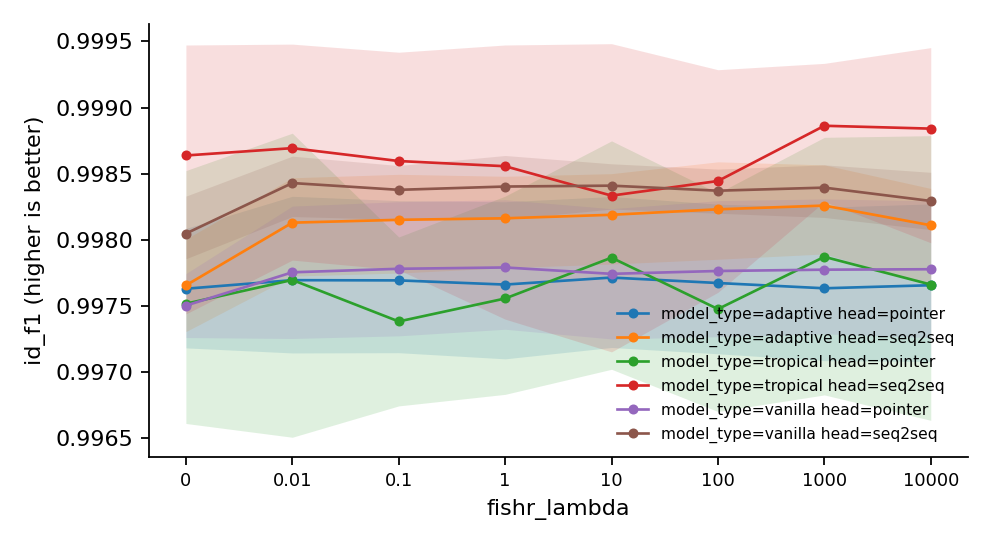
\includegraphics[width=\textwidth]{metric_id_f1.png}
\caption{\texttt{id\_f1} against \texttt{fishr\_lambda}: the mean over seeds with a 95\% bootstrap CI, one line per combination of the other factors.}
\label{fig:id_f1}
\end{figure}

{\small
\begin{longtable}{lllrlrrr}
\caption{\texttt{id\_f1} per cell: mean, 95\% bootstrap CI, SD, seeds, diverged runs.}\label{tab:summary-id_f1}\\
\toprule
\texttt{model\_type} & \texttt{head} & \texttt{fishr\_lambda} & mean & 95\% CI & SD & $n$ & div.\\
\midrule
\endhead
adaptive & pointer & 0 & 0.9976 & [0.997, 0.998] & $5.85\times10^{-4}$ & 5 & 0\\
adaptive & pointer & 0.01 & 0.9977 & [0.997, 0.998] & $7.63\times10^{-4}$ & 5 & 0\\
adaptive & pointer & 0.1 & 0.9977 & [0.997, 0.998] & $7.46\times10^{-4}$ & 5 & 0\\
adaptive & pointer & 1 & 0.9977 & [0.997, 0.998] & $7.78\times10^{-4}$ & 5 & 0\\
adaptive & pointer & 10 & 0.9977 & [0.997, 0.998] & $7.32\times10^{-4}$ & 5 & 0\\
adaptive & pointer & 100 & 0.9977 & [0.997, 0.998] & $7.34\times10^{-4}$ & 5 & 0\\
adaptive & pointer & 1000 & 0.9976 & [0.997, 0.998] & $7.40\times10^{-4}$ & 5 & 0\\
adaptive & pointer & 1e+04 & 0.9977 & [0.997, 0.998] & $7.71\times10^{-4}$ & 5 & 0\\
adaptive & seq2seq & 0 & 0.9977 & [0.997, 0.998] & $4.47\times10^{-4}$ & 5 & 0\\
adaptive & seq2seq & 0.01 & 0.9981 & [0.998, 0.998] & $4.71\times10^{-4}$ & 5 & 0\\
adaptive & seq2seq & 0.1 & 0.9981 & [0.998, 0.998] & $4.73\times10^{-4}$ & 5 & 0\\
adaptive & seq2seq & 1 & 0.9982 & [0.998, 0.998] & $4.36\times10^{-4}$ & 5 & 0\\
adaptive & seq2seq & 10 & 0.9982 & [0.998, 0.998] & $4.45\times10^{-4}$ & 5 & 0\\
adaptive & seq2seq & 100 & 0.9982 & [0.998, 0.999] & $4.75\times10^{-4}$ & 5 & 0\\
adaptive & seq2seq & 1000 & 0.9983 & [0.998, 0.999] & $4.59\times10^{-4}$ & 5 & 0\\
adaptive & seq2seq & 1e+04 & 0.9981 & [0.998, 0.998] & $4.99\times10^{-4}$ & 5 & 0\\
tropical & pointer & 0 & 0.9975 & [0.997, 0.999] & 0.00127 & 5 & 0\\
tropical & pointer & 0.01 & 0.9977 & [0.997, 0.999] & 0.00148 & 5 & 0\\
tropical & pointer & 0.1 & 0.9974 & [0.997, 0.998] & $8.13\times10^{-4}$ & 5 & 0\\
tropical & pointer & 1 & 0.9976 & [0.997, 0.998] & $9.58\times10^{-4}$ & 5 & 0\\
tropical & pointer & 10 & 0.9979 & [0.997, 0.999] & 0.00112 & 5 & 0\\
tropical & pointer & 100 & 0.9975 & [0.997, 0.998] & 0.00107 & 5 & 0\\
tropical & pointer & 1000 & 0.9979 & [0.997, 0.999] & 0.00123 & 5 & 0\\
tropical & pointer & 1e+04 & 0.9977 & [0.997, 0.999] & 0.00141 & 5 & 0\\
tropical & seq2seq & 0 & 0.9986 & [0.997, 0.999] & 0.00136 & 5 & 0\\
tropical & seq2seq & 0.01 & 0.9987 & [0.998, 0.999] & 0.00104 & 5 & 0\\
tropical & seq2seq & 0.1 & 0.9986 & [0.998, 0.999] & 0.00106 & 5 & 0\\
tropical & seq2seq & 1 & 0.9986 & [0.997, 0.999] & 0.00138 & 5 & 0\\
tropical & seq2seq & 10 & 0.9983 & [0.997, 0.999] & 0.00153 & 5 & 0\\
tropical & seq2seq & 100 & 0.9984 & [0.998, 0.999] & 0.00109 & 5 & 0\\
tropical & seq2seq & 1000 & 0.9989 & [0.998, 0.999] & $6.70\times10^{-4}$ & 5 & 0\\
tropical & seq2seq & 1e+04 & 0.9988 & [0.998, 0.999] & $9.64\times10^{-4}$ & 5 & 0\\
vanilla & pointer & 0 & 0.9975 & [0.997, 0.998] & $3.23\times10^{-4}$ & 5 & 0\\
vanilla & pointer & 0.01 & 0.9978 & [0.997, 0.998] & $6.56\times10^{-4}$ & 5 & 0\\
vanilla & pointer & 0.1 & 0.9978 & [0.997, 0.998] & $6.89\times10^{-4}$ & 5 & 0\\
vanilla & pointer & 1 & 0.9978 & [0.997, 0.998] & $6.48\times10^{-4}$ & 5 & 0\\
vanilla & pointer & 10 & 0.9977 & [0.997, 0.998] & $6.57\times10^{-4}$ & 5 & 0\\
vanilla & pointer & 100 & 0.9978 & [0.997, 0.998] & $6.58\times10^{-4}$ & 5 & 0\\
vanilla & pointer & 1000 & 0.9978 & [0.997, 0.998] & $6.51\times10^{-4}$ & 5 & 0\\
vanilla & pointer & 1e+04 & 0.9978 & [0.997, 0.998] & $6.86\times10^{-4}$ & 5 & 0\\
vanilla & seq2seq & 0 & 0.998 & [0.998, 0.998] & $3.13\times10^{-4}$ & 5 & 0\\
vanilla & seq2seq & 0.01 & 0.9984 & [0.998, 0.999] & $2.86\times10^{-4}$ & 5 & 0\\
vanilla & seq2seq & 0.1 & 0.9984 & [0.998, 0.999] & $2.56\times10^{-4}$ & 5 & 0\\
vanilla & seq2seq & 1 & 0.9984 & [0.998, 0.999] & $3.06\times10^{-4}$ & 5 & 0\\
vanilla & seq2seq & 10 & 0.9984 & [0.998, 0.999] & $2.41\times10^{-4}$ & 5 & 0\\
vanilla & seq2seq & 100 & 0.9984 & [0.998, 0.999] & $2.33\times10^{-4}$ & 5 & 0\\
vanilla & seq2seq & 1000 & 0.9984 & [0.998, 0.999] & $2.52\times10^{-4}$ & 5 & 0\\
vanilla & seq2seq & 1e+04 & 0.9983 & [0.998, 0.999] & $2.79\times10^{-4}$ & 5 & 0\\
\bottomrule
\end{longtable}
}

{\small
\begin{longtable}{lllrrrl}
\caption{\texttt{id\_f1}: each level of \texttt{fishr\_lambda} against its control (0), within each combination of the other factors. rank: Wilcoxon signed-rank by seed, Holm.}\label{tab:control-id_f1}\\
\toprule
\texttt{model\_type} & \texttt{head} & \texttt{fishr\_lambda} & difference & 95\% CI & $p$ & \\
\midrule
\endhead
adaptive & pointer & 0.01 & $8.380\times10^{-6}$ & [$-1.58\times10^{-4}$, $3.27\times10^{-4}$] & 1.0000 & \\
adaptive & pointer & 0.1 & $-8.239\times10^{-6}$ & [$-1.48\times10^{-4}$, $3.11\times10^{-4}$] & 1.0000 & \\
adaptive & pointer & 1 & $8.156\times10^{-6}$ & [$-1.75\times10^{-4}$, $2.84\times10^{-4}$] & 1.0000 & \\
adaptive & pointer & 10 & $2.812\times10^{-8}$ & [$-1.43\times10^{-4}$, $3.39\times10^{-4}$] & 1.0000 & \\
adaptive & pointer & 100 & $-4.137\times10^{-5}$ & [$-1.51\times10^{-4}$, $2.72\times10^{-4}$] & 1.0000 & \\
adaptive & pointer & 1000 & $-2.489\times10^{-5}$ & [$-1.76\times10^{-4}$, $2.24\times10^{-4}$] & 1.0000 & \\
adaptive & pointer & 1e+04 & $-1.654\times10^{-5}$ & [$-1.60\times10^{-4}$, $2.74\times10^{-4}$] & 1.0000 & \\
adaptive & seq2seq & 0.01 & $5.550\times10^{-4}$ & [$2.98\times10^{-4}$, $6.42\times10^{-4}$] & 0.4375 & \\
adaptive & seq2seq & 0.1 & $5.300\times10^{-4}$ & [$3.45\times10^{-4}$, $6.46\times10^{-4}$] & 0.4375 & \\
adaptive & seq2seq & 1 & $5.300\times10^{-4}$ & [$3.62\times10^{-4}$, $6.45\times10^{-4}$] & 0.4375 & \\
adaptive & seq2seq & 10 & $4.887\times10^{-4}$ & [$3.71\times10^{-4}$, $6.98\times10^{-4}$] & 0.4375 & \\
adaptive & seq2seq & 100 & $6.051\times10^{-4}$ & [$4.07\times10^{-4}$, $7.45\times10^{-4}$] & 0.4375 & \\
adaptive & seq2seq & 1000 & $7.210\times10^{-4}$ & [$3.86\times10^{-4}$, $8.21\times10^{-4}$] & 0.4375 & \\
adaptive & seq2seq & 1e+04 & $2.164\times10^{-4}$ & [$1.33\times10^{-4}$, $8.24\times10^{-4}$] & 0.4375 & \\
tropical & pointer & 0.01 & $-7.455\times10^{-4}$ & [$-8.14\times10^{-4}$, 0.0017] & 1.0000 & \\
tropical & pointer & 0.1 & $-3.577\times10^{-4}$ & [$-8.21\times10^{-4}$, $6.32\times10^{-4}$] & 1.0000 & \\
tropical & pointer & 1 & $1.756\times10^{-4}$ & [$-9.37\times10^{-4}$, $9.52\times10^{-4}$] & 1.0000 & \\
tropical & pointer & 10 & $4.259\times10^{-4}$ & [$-8.69\times10^{-4}$, 0.00145] & 1.0000 & \\
tropical & pointer & 100 & $-1.161\times10^{-4}$ & [$-8.18\times10^{-4}$, $7.36\times10^{-4}$] & 1.0000 & \\
tropical & pointer & 1000 & $5.794\times10^{-5}$ & [$-6.61\times10^{-4}$, 0.00135] & 1.0000 & \\
tropical & pointer & 1e+04 & $3.333\times10^{-5}$ & [-0.00124, 0.00169] & 1.0000 & \\
tropical & seq2seq & 0.01 & $8.283\times10^{-6}$ & [$-4.96\times10^{-4}$, $6.08\times10^{-4}$] & 1.0000 & \\
tropical & seq2seq & 0.1 & $-8.276\times10^{-6}$ & [$-7.44\times10^{-4}$, $5.77\times10^{-4}$] & 1.0000 & \\
tropical & seq2seq & 1 & 0 & [$-3.19\times10^{-4}$, $7.11\times10^{-5}$] & 1.0000 & \\
tropical & seq2seq & 10 & 0 & [-0.001, $8.60\times10^{-5}$] & 1.0000 & \\
tropical & seq2seq & 100 & $-1.159\times10^{-4}$ & [$-9.23\times10^{-4}$, $5.29\times10^{-4}$] & 1.0000 & \\
tropical & seq2seq & 1000 & $8.268\times10^{-6}$ & [$-2.21\times10^{-4}$, $9.04\times10^{-4}$] & 1.0000 & \\
tropical & seq2seq & 1e+04 & $8.268\times10^{-6}$ & [$-2.81\times10^{-5}$, $5.75\times10^{-4}$] & 1.0000 & \\
vanilla & pointer & 0.01 & $1.162\times10^{-4}$ & [$-7.21\times10^{-6}$, $5.06\times10^{-4}$] & 0.8750 & \\
vanilla & pointer & 0.1 & $4.961\times10^{-5}$ & [$1.28\times10^{-5}$, $5.74\times10^{-4}$] & 0.8750 & \\
vanilla & pointer & 1 & $1.578\times10^{-4}$ & [$3.78\times10^{-5}$, $5.39\times10^{-4}$] & 0.8750 & \\
vanilla & pointer & 10 & $7.419\times10^{-5}$ & [$-1.87\times10^{-5}$, $4.99\times10^{-4}$] & 0.8750 & \\
vanilla & pointer & 100 & $1.161\times10^{-4}$ & [$7.86\times10^{-6}$, $5.27\times10^{-4}$] & 0.8750 & \\
vanilla & pointer & 1000 & $1.079\times10^{-4}$ & [$2.76\times10^{-5}$, $5.16\times10^{-4}$] & 0.8750 & \\
vanilla & pointer & 1e+04 & $1.329\times10^{-4}$ & [$7.99\times10^{-6}$, $5.56\times10^{-4}$] & 0.8750 & \\
vanilla & seq2seq & 0.01 & $3.394\times10^{-4}$ & [$1.74\times10^{-4}$, $6.00\times10^{-4}$] & 0.4375 & \\
vanilla & seq2seq & 0.1 & $2.730\times10^{-4}$ & [$1.19\times10^{-4}$, $5.56\times10^{-4}$] & 0.4375 & \\
vanilla & seq2seq & 1 & $1.573\times10^{-4}$ & [$1.21\times10^{-4}$, $5.92\times10^{-4}$] & 0.4375 & \\
vanilla & seq2seq & 10 & $3.644\times10^{-4}$ & [$1.39\times10^{-4}$, $5.93\times10^{-4}$] & 0.4375 & \\
vanilla & seq2seq & 100 & $2.978\times10^{-4}$ & [$9.40\times10^{-5}$, $5.81\times10^{-4}$] & 0.4375 & \\
vanilla & seq2seq & 1000 & $3.973\times10^{-4}$ & [$1.52\times10^{-4}$, $5.53\times10^{-4}$] & 0.4375 & \\
vanilla & seq2seq & 1e+04 & $1.737\times10^{-4}$ & [$5.12\times10^{-5}$, $4.87\times10^{-4}$] & 0.4375 & \\
\bottomrule
\end{longtable}
}

{\small
\begin{longtable}{llrrrrr}
\caption{\texttt{id\_f1} against log10 \texttt{fishr\_lambda}: rank: Spearman rho, seed-bootstrap CI, with the Jonckheere--Terpstra ordered-trend $\tau$ and $p$.}\label{tab:trend-id_f1}\\
\toprule
\texttt{model\_type} & \texttt{head} & estimate & 95\% CI & $p$ & JT $\tau$ & JT $p$\\
\midrule
\endhead
adaptive & pointer & -0.1315 & [-0.439, 0.111] & 0.4513 & -0.0971 & 0.4673\\
adaptive & seq2seq & -0.01839 & [-0.143, 0.289] & 0.9165 & -0.00571 & 0.9764\\
tropical & pointer & 0.08063 & [-0.232, 0.318] & 0.6452 & 0.0743 & 0.5935\\
tropical & seq2seq & -0.01346 & [-0.19, 0.139] & 0.9388 & 0.00381 & 0.9826\\
vanilla & pointer & -0.008487 & [-0.221, 0.106] & 0.9614 & -0.0019 & 1.0000\\
vanilla & seq2seq & -0.1514 & [-0.429, 0.0113] & 0.3854 & -0.122 & 0.3739\\
\bottomrule
\end{longtable}
}

{\small
\begin{longtable}{lrrrl}
\caption{\texttt{id\_f1}: paired contrasts by seed, Holm-corrected across the cells. rank: Wilcoxon signed-rank by seed, Holm.}\label{tab:paired-id_f1}\\
\toprule
contrast (within) & difference & 95\% CI & $p$ & \\
\midrule
\endhead
\stackcell{model\_type: tropical - vanilla\\\footnotesize head=pointer fishr\_lambda=0 } & $1.428\times10^{-5}$ & [-0.0015, 0.00152] & 1.0000 & \\
\stackcell{model\_type: tropical - vanilla\\\footnotesize head=pointer fishr\_lambda=0.01 } & $-5.791\times10^{-5}$ & [-0.00122, 0.00111] & 1.0000 & \\
\stackcell{model\_type: tropical - vanilla\\\footnotesize head=pointer fishr\_lambda=0.1 } & $-3.987\times10^{-4}$ & [$-9.28\times10^{-4}$, $1.31\times10^{-4}$] & 1.0000 & \\
\stackcell{model\_type: tropical - vanilla\\\footnotesize head=pointer fishr\_lambda=1 } & $-2.349\times10^{-4}$ & [$-7.43\times10^{-4}$, $2.73\times10^{-4}$] & 1.0000 & \\
\stackcell{model\_type: tropical - vanilla\\\footnotesize head=pointer fishr\_lambda=10 } & $1.226\times10^{-4}$ & [-0.00107, 0.00131] & 1.0000 & \\
\stackcell{model\_type: tropical - vanilla\\\footnotesize head=pointer fishr\_lambda=100 } & $-2.883\times10^{-4}$ & [-0.00116, $5.88\times10^{-4}$] & 1.0000 & \\
\stackcell{model\_type: tropical - vanilla\\\footnotesize head=pointer fishr\_lambda=1000 } & $9.725\times10^{-5}$ & [$-9.56\times10^{-4}$, 0.00115] & 1.0000 & \\
\stackcell{model\_type: tropical - vanilla\\\footnotesize head=pointer fishr\_lambda=1e+04 } & $-1.159\times10^{-4}$ & [-0.00109, $8.57\times10^{-4}$] & 1.0000 & \\
\stackcell{model\_type: tropical - vanilla\\\footnotesize head=seq2seq fishr\_lambda=0 } & $5.912\times10^{-4}$ & [$-9.90\times10^{-4}$, 0.00217] & 1.0000 & \\
\stackcell{model\_type: tropical - vanilla\\\footnotesize head=seq2seq fishr\_lambda=0.01 } & $2.643\times10^{-4}$ & [$-7.48\times10^{-4}$, 0.00128] & 1.0000 & \\
\stackcell{model\_type: tropical - vanilla\\\footnotesize head=seq2seq fishr\_lambda=0.1 } & $2.181\times10^{-4}$ & [-0.00101, 0.00145] & 1.0000 & \\
\stackcell{model\_type: tropical - vanilla\\\footnotesize head=seq2seq fishr\_lambda=1 } & $1.538\times10^{-4}$ & [-0.00127, 0.00158] & 1.0000 & \\
\stackcell{model\_type: tropical - vanilla\\\footnotesize head=seq2seq fishr\_lambda=10 } & $-7.551\times10^{-5}$ & [-0.00175, 0.00159] & 1.0000 & \\
\stackcell{model\_type: tropical - vanilla\\\footnotesize head=seq2seq fishr\_lambda=100 } & $7.341\times10^{-5}$ & [-0.00101, 0.00116] & 1.0000 & \\
\stackcell{model\_type: tropical - vanilla\\\footnotesize head=seq2seq fishr\_lambda=1000 } & $4.685\times10^{-4}$ & [$-2.41\times10^{-4}$, 0.00118] & 1.0000 & \\
\stackcell{model\_type: tropical - vanilla\\\footnotesize head=seq2seq fishr\_lambda=1e+04 } & $5.478\times10^{-4}$ & [$-3.58\times10^{-4}$, 0.00145] & 1.0000 & \\
\stackcell{model\_type: adaptive - vanilla\\\footnotesize head=pointer fishr\_lambda=0 } & $1.276\times10^{-4}$ & [$-3.13\times10^{-4}$, $5.68\times10^{-4}$] & 1.0000 & \\
\stackcell{model\_type: adaptive - vanilla\\\footnotesize head=pointer fishr\_lambda=0.01 } & $-5.955\times10^{-5}$ & [$-3.24\times10^{-4}$, $2.05\times10^{-4}$] & 1.0000 & \\
\stackcell{model\_type: adaptive - vanilla\\\footnotesize head=pointer fishr\_lambda=0.1 } & $-8.782\times10^{-5}$ & [$-2.67\times10^{-4}$, $9.18\times10^{-5}$] & 1.0000 & \\
\stackcell{model\_type: adaptive - vanilla\\\footnotesize head=pointer fishr\_lambda=1 } & $-1.295\times10^{-4}$ & [$-4.36\times10^{-4}$, $1.77\times10^{-4}$] & 1.0000 & \\
\stackcell{model\_type: adaptive - vanilla\\\footnotesize head=pointer fishr\_lambda=10 } & $-2.815\times10^{-5}$ & [$-2.75\times10^{-4}$, $2.18\times10^{-4}$] & 1.0000 & \\
\stackcell{model\_type: adaptive - vanilla\\\footnotesize head=pointer fishr\_lambda=100 } & $-9.111\times10^{-5}$ & [$-3.02\times10^{-4}$, $1.19\times10^{-4}$] & 1.0000 & \\
\stackcell{model\_type: adaptive - vanilla\\\footnotesize head=pointer fishr\_lambda=1000 } & $-1.409\times10^{-4}$ & [$-4.20\times10^{-4}$, $1.38\times10^{-4}$] & 1.0000 & \\
\stackcell{model\_type: adaptive - vanilla\\\footnotesize head=pointer fishr\_lambda=1e+04 } & $-1.211\times10^{-4}$ & [$-4.16\times10^{-4}$, $1.74\times10^{-4}$] & 1.0000 & \\
\stackcell{model\_type: adaptive - vanilla\\\footnotesize head=seq2seq fishr\_lambda=0 } & $-3.922\times10^{-4}$ & [$-9.82\times10^{-4}$, $1.98\times10^{-4}$] & 1.0000 & \\
\stackcell{model\_type: adaptive - vanilla\\\footnotesize head=seq2seq fishr\_lambda=0.01 } & $-3.000\times10^{-4}$ & [$-5.43\times10^{-4}$, $-5.75\times10^{-5}$] & 1.0000 & \\
\stackcell{model\_type: adaptive - vanilla\\\footnotesize head=seq2seq fishr\_lambda=0.1 } & $-2.271\times10^{-4}$ & [$-5.04\times10^{-4}$, $4.96\times10^{-5}$] & 1.0000 & \\
\stackcell{model\_type: adaptive - vanilla\\\footnotesize head=seq2seq fishr\_lambda=1 } & $-2.405\times10^{-4}$ & [$-4.19\times10^{-4}$, $-6.15\times10^{-5}$] & 1.0000 & \\
\stackcell{model\_type: adaptive - vanilla\\\footnotesize head=seq2seq fishr\_lambda=10 } & $-2.206\times10^{-4}$ & [$-4.85\times10^{-4}$, $4.40\times10^{-5}$] & 1.0000 & \\
\stackcell{model\_type: adaptive - vanilla\\\footnotesize head=seq2seq fishr\_lambda=100 } & $-1.409\times10^{-4}$ & [$-4.72\times10^{-4}$, $1.91\times10^{-4}$] & 1.0000 & \\
\stackcell{model\_type: adaptive - vanilla\\\footnotesize head=seq2seq fishr\_lambda=1000 } & $-1.359\times10^{-4}$ & [$-4.01\times10^{-4}$, $1.29\times10^{-4}$] & 1.0000 & \\
\stackcell{model\_type: adaptive - vanilla\\\footnotesize head=seq2seq fishr\_lambda=1e+04 } & $-1.840\times10^{-4}$ & [$-7.56\times10^{-4}$, $3.88\times10^{-4}$] & 1.0000 & \\
\stackcell{head: pointer - seq2seq\\\footnotesize model\_type=adaptive fishr\_lambda=0 } & $-2.552\times10^{-5}$ & [$-4.25\times10^{-4}$, $3.74\times10^{-4}$] & 1.0000 & \\
\stackcell{head: pointer - seq2seq\\\footnotesize model\_type=adaptive fishr\_lambda=0.01 } & $-4.355\times10^{-4}$ & [-0.00112, $2.45\times10^{-4}$] & 1.0000 & \\
\stackcell{head: pointer - seq2seq\\\footnotesize model\_type=adaptive fishr\_lambda=0.1 } & $-4.586\times10^{-4}$ & [-0.00116, $2.39\times10^{-4}$] & 1.0000 & \\
\stackcell{head: pointer - seq2seq\\\footnotesize model\_type=adaptive fishr\_lambda=1 } & $-5.019\times10^{-4}$ & [-0.00126, $2.55\times10^{-4}$] & 1.0000 & \\
\stackcell{head: pointer - seq2seq\\\footnotesize model\_type=adaptive fishr\_lambda=10 } & $-4.753\times10^{-4}$ & [-0.00121, $2.61\times10^{-4}$] & 1.0000 & \\
\stackcell{head: pointer - seq2seq\\\footnotesize model\_type=adaptive fishr\_lambda=100 } & $-5.582\times10^{-4}$ & [-0.00109, $-2.33\times10^{-5}$] & 1.0000 & \\
\stackcell{head: pointer - seq2seq\\\footnotesize model\_type=adaptive fishr\_lambda=1000 } & $-6.263\times10^{-4}$ & [-0.00133, $7.97\times10^{-5}$] & 1.0000 & \\
\stackcell{head: pointer - seq2seq\\\footnotesize model\_type=adaptive fishr\_lambda=1e+04 } & $-4.540\times10^{-4}$ & [-0.00149, $5.79\times10^{-4}$] & 1.0000 & \\
\stackcell{head: pointer - seq2seq\\\footnotesize model\_type=tropical fishr\_lambda=0 } & -0.001122 & [-0.00388, 0.00163] & 1.0000 & \\
\stackcell{head: pointer - seq2seq\\\footnotesize model\_type=tropical fishr\_lambda=0.01 } & $-9.981\times10^{-4}$ & [-0.00271, $7.16\times10^{-4}$] & 1.0000 & \\
\stackcell{head: pointer - seq2seq\\\footnotesize model\_type=tropical fishr\_lambda=0.1 } & -0.001215 & [-0.00242, $-6.50\times10^{-6}$] & 1.0000 & \\
\stackcell{head: pointer - seq2seq\\\footnotesize model\_type=tropical fishr\_lambda=1 } & -0.001002 & [-0.00231, $3.03\times10^{-4}$] & 1.0000 & \\
\stackcell{head: pointer - seq2seq\\\footnotesize model\_type=tropical fishr\_lambda=10 } & $-4.697\times10^{-4}$ & [-0.00153, $5.91\times10^{-4}$] & 1.0000 & \\
\stackcell{head: pointer - seq2seq\\\footnotesize model\_type=tropical fishr\_lambda=100 } & $-9.696\times10^{-4}$ & [-0.00244, $5.00\times10^{-4}$] & 1.0000 & \\
\stackcell{head: pointer - seq2seq\\\footnotesize model\_type=tropical fishr\_lambda=1000 } & $-9.924\times10^{-4}$ & [-0.00204, $5.43\times10^{-5}$] & 1.0000 & \\
\stackcell{head: pointer - seq2seq\\\footnotesize model\_type=tropical fishr\_lambda=1e+04 } & -0.001181 & [-0.00247, $1.04\times10^{-4}$] & 1.0000 & \\
\stackcell{head: pointer - seq2seq\\\footnotesize model\_type=vanilla fishr\_lambda=0 } & $-5.453\times10^{-4}$ & [$-9.11\times10^{-4}$, $-1.80\times10^{-4}$] & 1.0000 & \\
\stackcell{head: pointer - seq2seq\\\footnotesize model\_type=vanilla fishr\_lambda=0.01 } & $-6.759\times10^{-4}$ & [-0.00124, $-1.10\times10^{-4}$] & 1.0000 & \\
\stackcell{head: pointer - seq2seq\\\footnotesize model\_type=vanilla fishr\_lambda=0.1 } & $-5.979\times10^{-4}$ & [-0.00124, $4.56\times10^{-5}$] & 1.0000 & \\
\stackcell{head: pointer - seq2seq\\\footnotesize model\_type=vanilla fishr\_lambda=1 } & $-6.129\times10^{-4}$ & [-0.00117, $-5.32\times10^{-5}$] & 1.0000 & \\
\stackcell{head: pointer - seq2seq\\\footnotesize model\_type=vanilla fishr\_lambda=10 } & $-6.678\times10^{-4}$ & [-0.00128, $-5.73\times10^{-5}$] & 1.0000 & \\
\stackcell{head: pointer - seq2seq\\\footnotesize model\_type=vanilla fishr\_lambda=100 } & $-6.079\times10^{-4}$ & [-0.00124, $2.80\times10^{-5}$] & 1.0000 & \\
\stackcell{head: pointer - seq2seq\\\footnotesize model\_type=vanilla fishr\_lambda=1000 } & $-6.212\times10^{-4}$ & [-0.00118, $-6.51\times10^{-5}$] & 1.0000 & \\
\stackcell{head: pointer - seq2seq\\\footnotesize model\_type=vanilla fishr\_lambda=1e+04 } & $-5.169\times10^{-4}$ & [-0.00112, $8.26\times10^{-5}$] & 1.0000 & \\
\bottomrule
\end{longtable}
}

\subsection{\texttt{id\_exact}}
\begin{figure}[tbp]
\centering
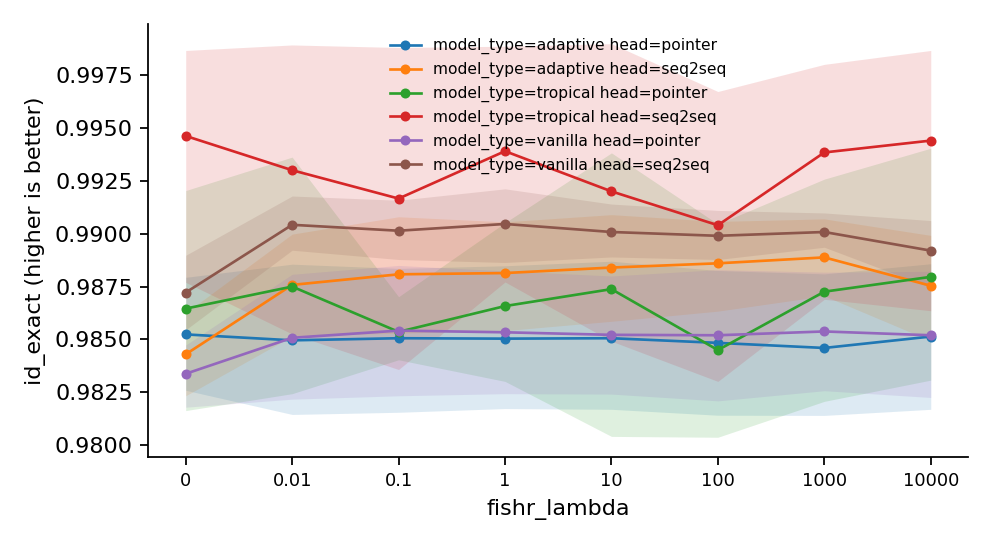
\includegraphics[width=\textwidth]{metric_id_exact.png}
\caption{\texttt{id\_exact} against \texttt{fishr\_lambda}: the mean over seeds with a 95\% bootstrap CI, one line per combination of the other factors.}
\label{fig:id_exact}
\end{figure}

{\small
\begin{longtable}{lllrlrrr}
\caption{\texttt{id\_exact} per cell: mean, 95\% bootstrap CI, SD, seeds, diverged runs.}\label{tab:summary-id_exact}\\
\toprule
\texttt{model\_type} & \texttt{head} & \texttt{fishr\_lambda} & mean & 95\% CI & SD & $n$ & div.\\
\midrule
\endhead
adaptive & pointer & 0 & 0.9852 & [0.983, 0.988] & 0.00349 & 5 & 0\\
adaptive & pointer & 0.01 & 0.985 & [0.981, 0.989] & 0.00456 & 5 & 0\\
adaptive & pointer & 0.1 & 0.9851 & [0.982, 0.988] & 0.00441 & 5 & 0\\
adaptive & pointer & 1 & 0.985 & [0.982, 0.988] & 0.00455 & 5 & 0\\
adaptive & pointer & 10 & 0.9851 & [0.982, 0.989] & 0.00423 & 5 & 0\\
adaptive & pointer & 100 & 0.9848 & [0.981, 0.988] & 0.00434 & 5 & 0\\
adaptive & pointer & 1000 & 0.9846 & [0.981, 0.988] & 0.00442 & 5 & 0\\
adaptive & pointer & 1e+04 & 0.9851 & [0.982, 0.989] & 0.00433 & 5 & 0\\
adaptive & seq2seq & 0 & 0.9843 & [0.982, 0.986] & 0.00248 & 5 & 0\\
adaptive & seq2seq & 0.01 & 0.9876 & [0.985, 0.99] & 0.0031 & 5 & 0\\
adaptive & seq2seq & 0.1 & 0.9881 & [0.985, 0.991] & 0.00356 & 5 & 0\\
adaptive & seq2seq & 1 & 0.9881 & [0.985, 0.991] & 0.00332 & 5 & 0\\
adaptive & seq2seq & 10 & 0.9884 & [0.986, 0.991] & 0.00319 & 5 & 0\\
adaptive & seq2seq & 100 & 0.9886 & [0.986, 0.991] & 0.00282 & 5 & 0\\
adaptive & seq2seq & 1000 & 0.9889 & [0.987, 0.991] & 0.00241 & 5 & 0\\
adaptive & seq2seq & 1e+04 & 0.9875 & [0.985, 0.99] & 0.00324 & 5 & 0\\
tropical & pointer & 0 & 0.9865 & [0.982, 0.992] & 0.00664 & 5 & 0\\
tropical & pointer & 0.01 & 0.9875 & [0.982, 0.994] & 0.00718 & 5 & 0\\
tropical & pointer & 0.1 & 0.9854 & [0.984, 0.987] & 0.0019 & 5 & 0\\
tropical & pointer & 1 & 0.9866 & [0.983, 0.991] & 0.00493 & 5 & 0\\
tropical & pointer & 10 & 0.9874 & [0.98, 0.994] & 0.00908 & 5 & 0\\
tropical & pointer & 100 & 0.9845 & [0.98, 0.99] & 0.0066 & 5 & 0\\
tropical & pointer & 1000 & 0.9873 & [0.982, 0.993] & 0.007 & 5 & 0\\
tropical & pointer & 1e+04 & 0.988 & [0.983, 0.994] & 0.00719 & 5 & 0\\
tropical & seq2seq & 0 & 0.9946 & [0.988, 0.999] & 0.00779 & 5 & 0\\
tropical & seq2seq & 0.01 & 0.993 & [0.985, 0.999] & 0.00874 & 5 & 0\\
tropical & seq2seq & 0.1 & 0.9917 & [0.984, 0.999] & 0.00977 & 5 & 0\\
tropical & seq2seq & 1 & 0.9939 & [0.988, 0.999] & 0.00782 & 5 & 0\\
tropical & seq2seq & 10 & 0.992 & [0.985, 0.999] & 0.00939 & 5 & 0\\
tropical & seq2seq & 100 & 0.9904 & [0.983, 0.997] & 0.00894 & 5 & 0\\
tropical & seq2seq & 1000 & 0.9938 & [0.987, 0.998] & 0.00759 & 5 & 0\\
tropical & seq2seq & 1e+04 & 0.9944 & [0.986, 0.999] & 0.00895 & 5 & 0\\
vanilla & pointer & 0 & 0.9834 & [0.982, 0.985] & 0.00178 & 5 & 0\\
vanilla & pointer & 0.01 & 0.9851 & [0.982, 0.988] & 0.00395 & 5 & 0\\
vanilla & pointer & 0.1 & 0.9854 & [0.982, 0.988] & 0.00402 & 5 & 0\\
vanilla & pointer & 1 & 0.9853 & [0.982, 0.988] & 0.00378 & 5 & 0\\
vanilla & pointer & 10 & 0.9852 & [0.982, 0.988] & 0.00369 & 5 & 0\\
vanilla & pointer & 100 & 0.9852 & [0.982, 0.988] & 0.00397 & 5 & 0\\
vanilla & pointer & 1000 & 0.9854 & [0.983, 0.988] & 0.00373 & 5 & 0\\
vanilla & pointer & 1e+04 & 0.9852 & [0.982, 0.988] & 0.004 & 5 & 0\\
vanilla & seq2seq & 0 & 0.9872 & [0.985, 0.989] & 0.00231 & 5 & 0\\
vanilla & seq2seq & 0.01 & 0.9904 & [0.989, 0.992] & 0.00154 & 5 & 0\\
vanilla & seq2seq & 0.1 & 0.9901 & [0.989, 0.992] & 0.0018 & 5 & 0\\
vanilla & seq2seq & 1 & 0.9905 & [0.989, 0.992] & 0.00225 & 5 & 0\\
vanilla & seq2seq & 10 & 0.9901 & [0.989, 0.991] & 0.00169 & 5 & 0\\
vanilla & seq2seq & 100 & 0.9899 & [0.989, 0.991] & 0.00151 & 5 & 0\\
vanilla & seq2seq & 1000 & 0.9901 & [0.989, 0.991] & 0.00105 & 5 & 0\\
vanilla & seq2seq & 1e+04 & 0.9892 & [0.987, 0.991] & 0.00209 & 5 & 0\\
\bottomrule
\end{longtable}
}

{\small
\begin{longtable}{lllrrrl}
\caption{\texttt{id\_exact}: each level of \texttt{fishr\_lambda} against its control (0), within each combination of the other factors. rank: Wilcoxon signed-rank by seed, Holm.}\label{tab:control-id_exact}\\
\toprule
\texttt{model\_type} & \texttt{head} & \texttt{fishr\_lambda} & difference & 95\% CI & $p$ & \\
\midrule
\endhead
adaptive & pointer & 0.01 & $-9.000\times10^{-4}$ & [-0.00146, 0.00124] & 1.0000 & \\
adaptive & pointer & 0.1 & $-6.000\times10^{-4}$ & [-0.00144, 0.00112] & 1.0000 & \\
adaptive & pointer & 1 & $-7.000\times10^{-4}$ & [-0.00138, 0.00102] & 1.0000 & \\
adaptive & pointer & 10 & $-5.000\times10^{-4}$ & [-0.00124, 0.00108] & 1.0000 & \\
adaptive & pointer & 100 & $-4.000\times10^{-4}$ & [-0.00144, $9.00\times10^{-4}$] & 1.0000 & \\
adaptive & pointer & 1000 & $-6.000\times10^{-4}$ & [-0.0018, $5.20\times10^{-4}$] & 1.0000 & \\
adaptive & pointer & 1e+04 & 0 & [-0.00128, 0.00114] & 1.0000 & \\
adaptive & seq2seq & 0.01 & 0.0028 & [0.00188, 0.00468] & 0.4375 & \\
adaptive & seq2seq & 0.1 & 0.0036 & [0.00228, 0.00526] & 0.4375 & \\
adaptive & seq2seq & 1 & 0.0029 & [0.00258, 0.00518] & 0.4375 & \\
adaptive & seq2seq & 10 & 0.0039 & [0.00268, 0.00532] & 0.4375 & \\
adaptive & seq2seq & 100 & 0.0035 & [0.00286, 0.00594] & 0.4375 & \\
adaptive & seq2seq & 1000 & 0.0052 & [0.00284, 0.00618] & 0.4375 & \\
adaptive & seq2seq & 1e+04 & 0.0018 & [$6.00\times10^{-4}$, 0.00594] & 0.4375 & \\
tropical & pointer & 0.01 & $-5.000\times10^{-4}$ & [-0.0052, 0.00958] & 1.0000 & \\
tropical & pointer & 0.1 & 0.0011 & [-0.0053, 0.00248] & 1.0000 & \\
tropical & pointer & 1 & $3.000\times10^{-4}$ & [-0.00538, 0.0051] & 1.0000 & \\
tropical & pointer & 10 & 0.0019 & [-0.00926, 0.00966] & 1.0000 & \\
tropical & pointer & 100 & $-4.000\times10^{-4}$ & [-0.00718, 0.0018] & 1.0000 & \\
tropical & pointer & 1000 & $4.000\times10^{-4}$ & [-0.006, 0.00644] & 1.0000 & \\
tropical & pointer & 1e+04 & 0 & [-0.00643, 0.0103] & 1.0000 & \\
tropical & seq2seq & 0.01 & $-1.000\times10^{-4}$ & [-0.00514, $8.80\times10^{-4}$] & 1.0000 & \\
tropical & seq2seq & 0.1 & $-3.000\times10^{-4}$ & [-0.00848, $7.40\times10^{-4}$] & 1.0000 & \\
tropical & seq2seq & 1 & 0 & [-0.00334, 0.00114] & 1.0000 & \\
tropical & seq2seq & 10 & 0 & [-0.00922, 0.00132] & 1.0000 & \\
tropical & seq2seq & 100 & -0.0025 & [-0.0097, $-2.40\times10^{-4}$] & 1.0000 & \\
tropical & seq2seq & 1000 & $-3.000\times10^{-4}$ & [-0.0027, $9.40\times10^{-4}$] & 1.0000 & \\
tropical & seq2seq & 1e+04 & 0 & [-0.00148, 0.00114] & 1.0000 & \\
vanilla & pointer & 0.01 & $4.000\times10^{-4}$ & [$-2.00\times10^{-4}$, 0.0036] & 0.9375 & \\
vanilla & pointer & 0.1 & $6.000\times10^{-4}$ & [$1.60\times10^{-4}$, 0.00392] & 0.8750 & \\
vanilla & pointer & 1 & $7.000\times10^{-4}$ & [$2.20\times10^{-4}$, 0.00378] & 0.8750 & \\
vanilla & pointer & 10 & $7.000\times10^{-4}$ & [$1.40\times10^{-4}$, 0.00354] & 0.8750 & \\
vanilla & pointer & 100 & $4.000\times10^{-4}$ & [$-2.00\times10^{-5}$, 0.00368] & 0.9375 & \\
vanilla & pointer & 1000 & 0.001 & [$2.40\times10^{-4}$, 0.00376] & 0.8750 & \\
vanilla & pointer & 1e+04 & $6.000\times10^{-4}$ & [$-1.20\times10^{-4}$, 0.00376] & 0.9375 & \\
vanilla & seq2seq & 0.01 & 0.0037 & [0.0016, 0.00482] & 0.4375 & \\
vanilla & seq2seq & 0.1 & 0.0035 & [0.00102, 0.0047] & 0.5000 & \\
vanilla & seq2seq & 1 & 0.0025 & [0.0013, 0.00538] & 0.4375 & \\
vanilla & seq2seq & 10 & 0.0035 & [$1.00\times10^{-3}$, 0.00458] & 0.5000 & \\
vanilla & seq2seq & 100 & 0.0034 & [$9.20\times10^{-4}$, 0.00444] & 0.5000 & \\
vanilla & seq2seq & 1000 & 0.0032 & [0.00116, 0.00456] & 0.4375 & \\
vanilla & seq2seq & 1e+04 & 0.0017 & [$6.00\times10^{-4}$, 0.00356] & 0.5000 & \\
\bottomrule
\end{longtable}
}

{\small
\begin{longtable}{llrrrrr}
\caption{\texttt{id\_exact} against log10 \texttt{fishr\_lambda}: rank: Spearman rho, seed-bootstrap CI, with the Jonckheere--Terpstra ordered-trend $\tau$ and $p$.}\label{tab:trend-id_exact}\\
\toprule
\texttt{model\_type} & \texttt{head} & estimate & 95\% CI & $p$ & JT $\tau$ & JT $p$\\
\midrule
\endhead
adaptive & pointer & 0.009203 & [-0.206, 0.122] & 0.9582 & 0.00762 & 0.9626\\
adaptive & seq2seq & 0.06296 & [-0.191, 0.381] & 0.7194 & 0.0324 & 0.8204\\
tropical & pointer & -0.01344 & [-0.359, 0.256] & 0.9389 & 0 & 1.0000\\
tropical & seq2seq & -0.04608 & [-0.304, 0.234] & 0.7926 & -0.0248 & 0.8542\\
vanilla & pointer & 0.01417 & [-0.156, 0.144] & 0.9356 & 0.00952 & 0.9478\\
vanilla & seq2seq & -0.1382 & [-0.38, -0.0639] & 0.4286 & -0.107 & 0.4231\\
\bottomrule
\end{longtable}
}

{\small
\begin{longtable}{lrrrl}
\caption{\texttt{id\_exact}: paired contrasts by seed, Holm-corrected across the cells. rank: Wilcoxon signed-rank by seed, Holm.}\label{tab:paired-id_exact}\\
\toprule
contrast (within) & difference & 95\% CI & $p$ & \\
\midrule
\endhead
\stackcell{model\_type: tropical - vanilla\\\footnotesize head=pointer fishr\_lambda=0 } & 0.00308 & [-0.00557, 0.0117] & 1.0000 & \\
\stackcell{model\_type: tropical - vanilla\\\footnotesize head=pointer fishr\_lambda=0.01 } & 0.00242 & [-0.00336, 0.0082] & 1.0000 & \\
\stackcell{model\_type: tropical - vanilla\\\footnotesize head=pointer fishr\_lambda=0.1 } & $-6.000\times10^{-5}$ & [-0.00473, 0.00461] & 1.0000 & \\
\stackcell{model\_type: tropical - vanilla\\\footnotesize head=pointer fishr\_lambda=1 } & 0.00124 & [-0.00162, 0.0041] & 1.0000 & \\
\stackcell{model\_type: tropical - vanilla\\\footnotesize head=pointer fishr\_lambda=10 } & 0.00216 & [-0.00836, 0.0127] & 1.0000 & \\
\stackcell{model\_type: tropical - vanilla\\\footnotesize head=pointer fishr\_lambda=100 } & $-7.000\times10^{-4}$ & [-0.0061, 0.0047] & 1.0000 & \\
\stackcell{model\_type: tropical - vanilla\\\footnotesize head=pointer fishr\_lambda=1000 } & 0.00188 & [-0.00548, 0.00924] & 1.0000 & \\
\stackcell{model\_type: tropical - vanilla\\\footnotesize head=pointer fishr\_lambda=1e+04 } & 0.00276 & [-0.00266, 0.00818] & 1.0000 & \\
\stackcell{model\_type: tropical - vanilla\\\footnotesize head=seq2seq fishr\_lambda=0 } & 0.0074 & [$-5.70\times10^{-4}$, 0.0154] & 1.0000 & \\
\stackcell{model\_type: tropical - vanilla\\\footnotesize head=seq2seq fishr\_lambda=0.01 } & 0.00258 & [-0.00695, 0.0121] & 1.0000 & \\
\stackcell{model\_type: tropical - vanilla\\\footnotesize head=seq2seq fishr\_lambda=0.1 } & 0.00152 & [-0.0109, 0.0139] & 1.0000 & \\
\stackcell{model\_type: tropical - vanilla\\\footnotesize head=seq2seq fishr\_lambda=1 } & 0.00344 & [-0.00425, 0.0111] & 1.0000 & \\
\stackcell{model\_type: tropical - vanilla\\\footnotesize head=seq2seq fishr\_lambda=10 } & 0.00192 & [-0.00905, 0.0129] & 1.0000 & \\
\stackcell{model\_type: tropical - vanilla\\\footnotesize head=seq2seq fishr\_lambda=100 } & $5.000\times10^{-4}$ & [-0.00943, 0.0104] & 1.0000 & \\
\stackcell{model\_type: tropical - vanilla\\\footnotesize head=seq2seq fishr\_lambda=1000 } & 0.00376 & [-0.00479, 0.0123] & 1.0000 & \\
\stackcell{model\_type: tropical - vanilla\\\footnotesize head=seq2seq fishr\_lambda=1e+04 } & 0.0052 & [-0.00366, 0.0141] & 1.0000 & \\
\stackcell{model\_type: adaptive - vanilla\\\footnotesize head=pointer fishr\_lambda=0 } & 0.00186 & [$-4.25\times10^{-4}$, 0.00415] & 1.0000 & \\
\stackcell{model\_type: adaptive - vanilla\\\footnotesize head=pointer fishr\_lambda=0.01 } & $-1.200\times10^{-4}$ & [-0.00191, 0.00167] & 1.0000 & \\
\stackcell{model\_type: adaptive - vanilla\\\footnotesize head=pointer fishr\_lambda=0.1 } & $-3.600\times10^{-4}$ & [-0.00146, $7.39\times10^{-4}$] & 1.0000 & \\
\stackcell{model\_type: adaptive - vanilla\\\footnotesize head=pointer fishr\_lambda=1 } & $-3.000\times10^{-4}$ & [-0.00187, 0.00127] & 1.0000 & \\
\stackcell{model\_type: adaptive - vanilla\\\footnotesize head=pointer fishr\_lambda=10 } & $-1.600\times10^{-4}$ & [-0.00181, 0.00149] & 1.0000 & \\
\stackcell{model\_type: adaptive - vanilla\\\footnotesize head=pointer fishr\_lambda=100 } & $-3.600\times10^{-4}$ & [-0.00157, $8.46\times10^{-4}$] & 1.0000 & \\
\stackcell{model\_type: adaptive - vanilla\\\footnotesize head=pointer fishr\_lambda=1000 } & $-7.800\times10^{-4}$ & [-0.00243, $8.68\times10^{-4}$] & 1.0000 & \\
\stackcell{model\_type: adaptive - vanilla\\\footnotesize head=pointer fishr\_lambda=1e+04 } & $-6.000\times10^{-5}$ & [-0.00183, 0.00171] & 1.0000 & \\
\stackcell{model\_type: adaptive - vanilla\\\footnotesize head=seq2seq fishr\_lambda=0 } & -0.00292 & [-0.00724, 0.0014] & 1.0000 & \\
\stackcell{model\_type: adaptive - vanilla\\\footnotesize head=seq2seq fishr\_lambda=0.01 } & -0.00284 & [-0.00545, $-2.29\times10^{-4}$] & 1.0000 & \\
\stackcell{model\_type: adaptive - vanilla\\\footnotesize head=seq2seq fishr\_lambda=0.1 } & -0.00206 & [-0.00533, 0.00121] & 1.0000 & \\
\stackcell{model\_type: adaptive - vanilla\\\footnotesize head=seq2seq fishr\_lambda=1 } & -0.00232 & [-0.00401, $-6.30\times10^{-4}$] & 1.0000 & \\
\stackcell{model\_type: adaptive - vanilla\\\footnotesize head=seq2seq fishr\_lambda=10 } & -0.00168 & [-0.00462, 0.00126] & 1.0000 & \\
\stackcell{model\_type: adaptive - vanilla\\\footnotesize head=seq2seq fishr\_lambda=100 } & -0.0013 & [-0.00395, 0.00135] & 1.0000 & \\
\stackcell{model\_type: adaptive - vanilla\\\footnotesize head=seq2seq fishr\_lambda=1000 } & -0.0012 & [-0.00343, 0.00103] & 1.0000 & \\
\stackcell{model\_type: adaptive - vanilla\\\footnotesize head=seq2seq fishr\_lambda=1e+04 } & -0.00166 & [-0.00648, 0.00316] & 1.0000 & \\
\stackcell{head: pointer - seq2seq\\\footnotesize model\_type=adaptive fishr\_lambda=0 } & $9.400\times10^{-4}$ & [-0.00286, 0.00474] & 1.0000 & \\
\stackcell{head: pointer - seq2seq\\\footnotesize model\_type=adaptive fishr\_lambda=0.01 } & -0.00262 & [-0.00805, 0.00281] & 1.0000 & \\
\stackcell{head: pointer - seq2seq\\\footnotesize model\_type=adaptive fishr\_lambda=0.1 } & -0.00302 & [-0.00868, 0.00264] & 1.0000 & \\
\stackcell{head: pointer - seq2seq\\\footnotesize model\_type=adaptive fishr\_lambda=1 } & -0.0031 & [-0.00876, 0.00256] & 1.0000 & \\
\stackcell{head: pointer - seq2seq\\\footnotesize model\_type=adaptive fishr\_lambda=10 } & -0.00334 & [-0.00914, 0.00246] & 1.0000 & \\
\stackcell{head: pointer - seq2seq\\\footnotesize model\_type=adaptive fishr\_lambda=100 } & -0.00376 & [-0.00813, $6.08\times10^{-4}$] & 1.0000 & \\
\stackcell{head: pointer - seq2seq\\\footnotesize model\_type=adaptive fishr\_lambda=1000 } & -0.00428 & [-0.00956, 0.001] & 1.0000 & \\
\stackcell{head: pointer - seq2seq\\\footnotesize model\_type=adaptive fishr\_lambda=1e+04 } & -0.0024 & [-0.0106, 0.00584] & 1.0000 & \\
\stackcell{head: pointer - seq2seq\\\footnotesize model\_type=tropical fishr\_lambda=0 } & -0.00816 & [-0.0235, 0.00713] & 1.0000 & \\
\stackcell{head: pointer - seq2seq\\\footnotesize model\_type=tropical fishr\_lambda=0.01 } & -0.0055 & [-0.0166, 0.00557] & 1.0000 & \\
\stackcell{head: pointer - seq2seq\\\footnotesize model\_type=tropical fishr\_lambda=0.1 } & -0.0063 & [-0.0184, 0.00576] & 1.0000 & \\
\stackcell{head: pointer - seq2seq\\\footnotesize model\_type=tropical fishr\_lambda=1 } & -0.00732 & [-0.0134, -0.00124] & 1.0000 & \\
\stackcell{head: pointer - seq2seq\\\footnotesize model\_type=tropical fishr\_lambda=10 } & -0.00462 & [-0.0117, 0.00241] & 1.0000 & \\
\stackcell{head: pointer - seq2seq\\\footnotesize model\_type=tropical fishr\_lambda=100 } & -0.0059 & [-0.0146, 0.00277] & 1.0000 & \\
\stackcell{head: pointer - seq2seq\\\footnotesize model\_type=tropical fishr\_lambda=1000 } & -0.00658 & [-0.0129, $-2.21\times10^{-4}$] & 1.0000 & \\
\stackcell{head: pointer - seq2seq\\\footnotesize model\_type=tropical fishr\_lambda=1e+04 } & -0.00644 & [-0.0163, 0.00338] & 1.0000 & \\
\stackcell{head: pointer - seq2seq\\\footnotesize model\_type=vanilla fishr\_lambda=0 } & -0.00384 & [-0.00683, $-8.51\times10^{-4}$] & 1.0000 & \\
\stackcell{head: pointer - seq2seq\\\footnotesize model\_type=vanilla fishr\_lambda=0.01 } & -0.00534 & [-0.0104, $-2.40\times10^{-4}$] & 1.0000 & \\
\stackcell{head: pointer - seq2seq\\\footnotesize model\_type=vanilla fishr\_lambda=0.1 } & -0.00472 & [-0.0106, 0.00112] & 1.0000 & \\
\stackcell{head: pointer - seq2seq\\\footnotesize model\_type=vanilla fishr\_lambda=1 } & -0.00512 & [-0.00991, $-3.35\times10^{-4}$] & 1.0000 & \\
\stackcell{head: pointer - seq2seq\\\footnotesize model\_type=vanilla fishr\_lambda=10 } & -0.00486 & [-0.0102, $4.63\times10^{-4}$] & 1.0000 & \\
\stackcell{head: pointer - seq2seq\\\footnotesize model\_type=vanilla fishr\_lambda=100 } & -0.0047 & [-0.0101, $6.94\times10^{-4}$] & 1.0000 & \\
\stackcell{head: pointer - seq2seq\\\footnotesize model\_type=vanilla fishr\_lambda=1000 } & -0.0047 & [-0.00958, $1.77\times10^{-4}$] & 1.0000 & \\
\stackcell{head: pointer - seq2seq\\\footnotesize model\_type=vanilla fishr\_lambda=1e+04 } & -0.004 & [-0.00921, 0.00121] & 1.0000 & \\
\bottomrule
\end{longtable}
}


\section{Curves}
\begin{figure}[tbp]
\centering
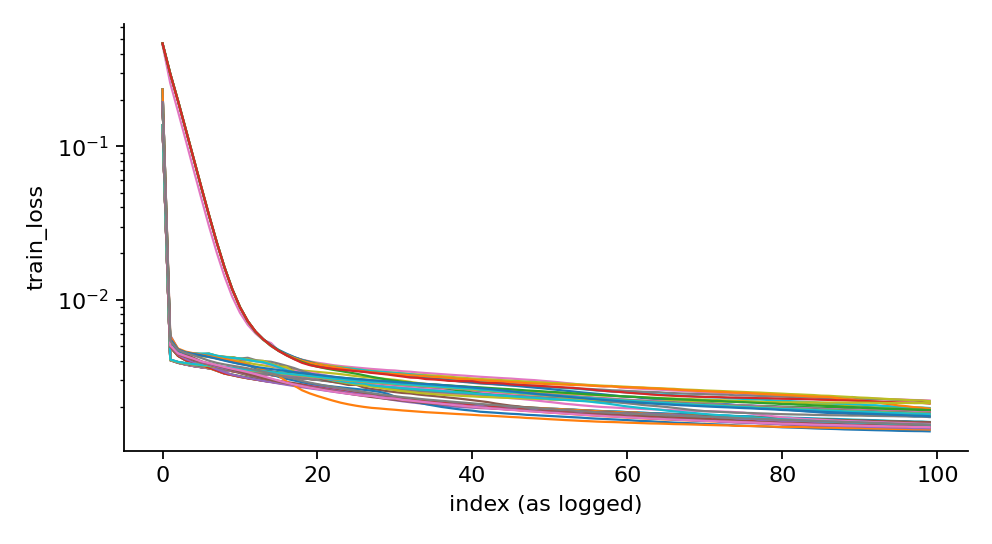
\includegraphics[width=\textwidth]{curve_train_loss.png}
\caption{\texttt{train\_loss}, the mean over seeds per cell.}
\label{fig:curve-1}
\end{figure}
\begin{figure}[tbp]
\centering
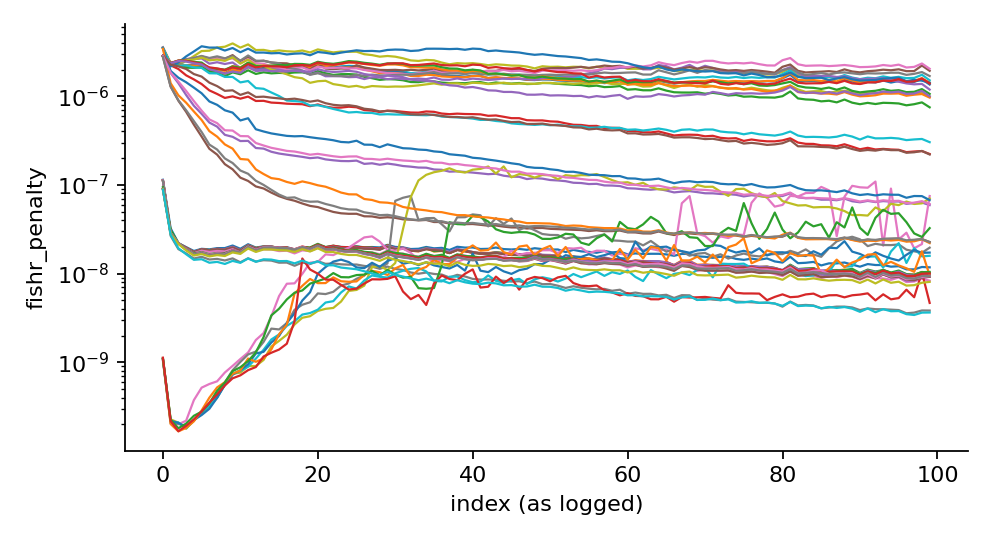
\includegraphics[width=\textwidth]{curve_fishr_penalty.png}
\caption{\texttt{fishr\_penalty}, the mean over seeds per cell.}
\label{fig:curve-2}
\end{figure}
\begin{figure}[tbp]
\centering
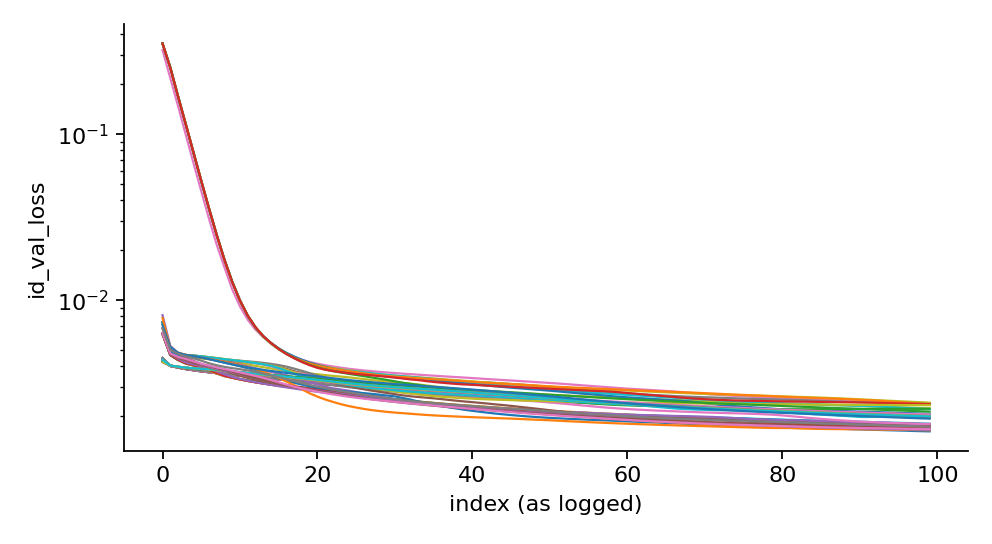
\includegraphics[width=\textwidth]{curve_id_val_loss.png}
\caption{\texttt{id\_val\_loss}, the mean over seeds per cell.}
\label{fig:curve-3}
\end{figure}

\section{Configuration}
The base configuration every run shares (frozen hash \texttt{0ea3d4b19330}); factor levels are in \autoref{tab:summary-ood_len_f1}.
{\footnotesize
\begin{verbatim}
task:
  name: SCCDataset
  value_range: 0.001
  target_range: null
  weight_range: null
  adversarial_range: null
  noise_prob: 0.0
data:
  train_lengths:
  - 4
  - 5
  - 6
  - 7
  - 8
  ood_lengths:
  - 12
  - 16
  ood_value_range: 0.1
  ood_noise_range: null
  ood_noise_prob: 0.5
  n_per_length: 20000
  n_eval_per_length: 2000
  curve_eval_limit: 256
model:
  d_model: 64
  n_heads: 2
  num_layers: 1
  dropout: 0.0
  tropical_impl: legacy
optim:
  lr: 0.0001
  epochs: 100
  batch_size: 8
  eval_batch_size: 8
fishr:
  ema: 0.95
  anneal_iters: 1500
  reset_optimizer: true
\end{verbatim}
}
Store: \texttt{campaigns/tropical/SCC/results}.
\end{document}